\section{信号优化}\label{sec:signal_optimization}
在初步筛选之后,为了进一步加强信号显著性,利用动力学性质进行信号优化是有必要的。因为每个信号质量点的动力学性质差别
较大,所以,每个质量点都会进行信号优化过程,而后通过各自
动力学选择条件之后的区域才作为每个质量点的最终信号区。

\subsection{优化策略}
MVA方法用于确定不同运动学变量的分离能力,并考虑所有变量之间的相关性。最终,前五个运动学变量用于形成优化选择,分别是$M(\ell\ell)$,$\Delta R_{min}(\ell_{2}, j)$,$\Delta R_{min}(\ell_{1}, j)$ ,$ M_{\ell_{1} jj}$和$M(all)$,它们具有很强的分离能力,而且相互之间的相关性很低(图~\ref{fig:correlation_check})。通常,$M(\ell\ell)$和$ M_{\ell_{1} jj} $对低质量点敏感,而其余对高质量和非共振信号敏感。
基于这些知识,$\Delta R_{min}(\ell_{1}, j)$,$M(\ell\ell)$,$ M_{\ell_{1}jj}$和$M(all)$用于在低质量搜索中形成优化削减,而$\Delta R_{min}(\ell_{2}, j)$,$\Delta R_{min}(\ell_{1}, j)$,$M(\ell\ell)$和$M_{\ell_{1}jj}$用于高质量搜索中。它们的相应分布分别见图~\ref{fig:SigOpt_low_kine}和图~\ref{fig:SigOpt_high_kine}。\\
TMVA包(CutsSA选项)~\cite{Hocker:2007ht}用于实现最佳筛选。所有背景:promptSS,$V\gamma$,QmisID和fakes都包含在训练中。
为了减少对变量筛选顺序的依赖,每次仅训练2个变量。
在每个信号效率工作点(WP),在测试样本中对每个事例应用对应的选择条件,
并计算显著性($S/\sqrt{B}$)。随后,选择具有最高信号显著性的WP,对应该WP的2个变量筛选值即为最佳选择,
最后再对剩下两个变量重复以上步骤。图~\ref{fig:nonres:SigOpt_mumu}展示SM希格斯粒子对搜寻中$\mu\mu$分析道的效率,各个运动学
变量的选择上下限以及显著性随信号效率WP的分布。
对剩余的分析道或者其他质量点重复此操作,即可得到所有质量点的分析道的最佳优化选择条件。值得指出的是,对于$SS$信号优化,因为各个质量点之间的运动学性质比较接近,所以只针对$m_S=135$~GeV, $m_X=300$~GeV ($m_X=340$~GeV, $m_S=145$~GeV)进行优化,而后应用在所有的低(高)质量点。 \\
最终考虑从低到高(和非共振)质量点筛选值的单调性,一定的选择调整被执行。最终的选择总结在表~\ref{optimization_cuts_lowmass},表~\ref {optimization_cuts_highmass}和表~\ref{optimization_cuts_HSS}中,分别对应于$hh$低质量,$hh$高质量和$SS$信号寻找。

\begin{figure}[h]
\centering
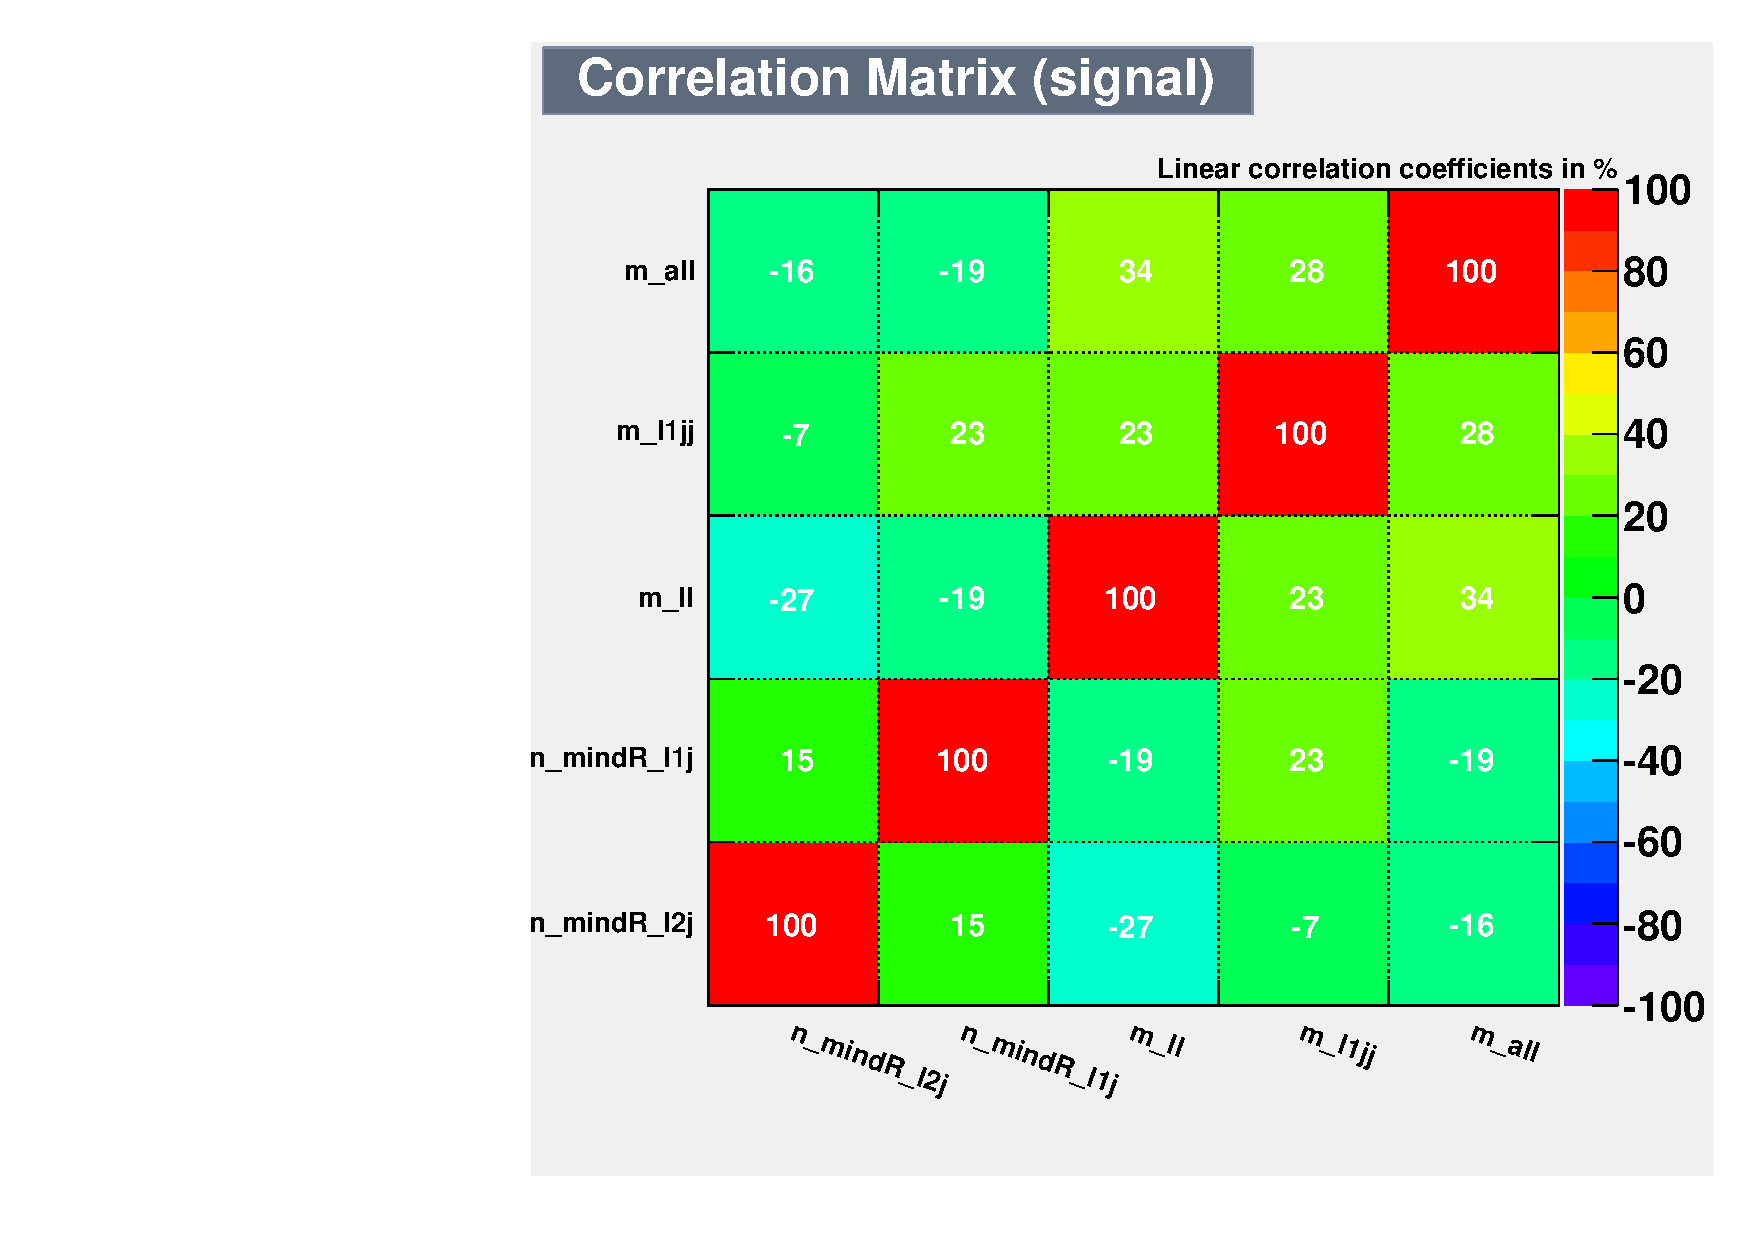
\includegraphics[width = 0.4\textwidth,angle=-90]{fig/SigOpt/correlation_signal.pdf}
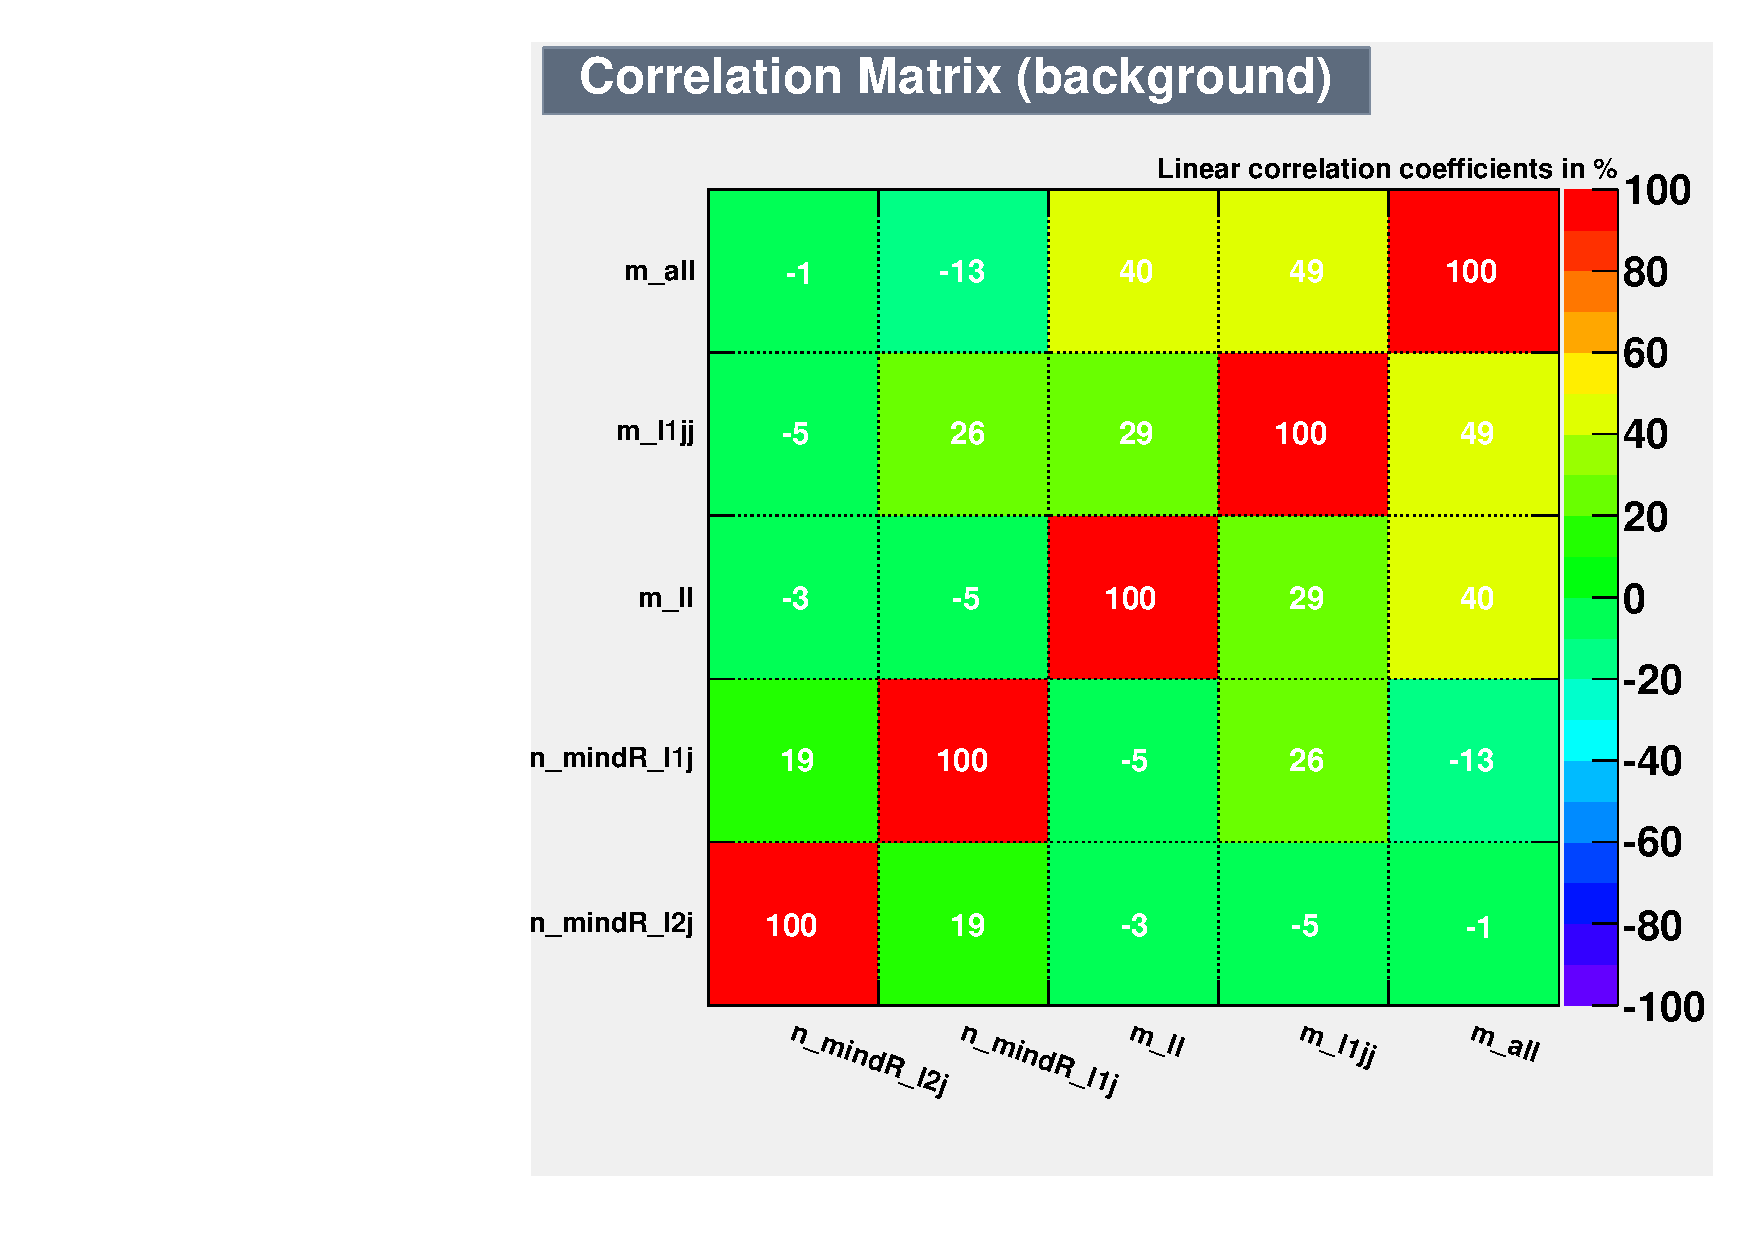
\includegraphics[width = 0.4\textwidth,angle=-90]{fig/SigOpt/correlation_bkg.pdf}
\caption{训练变量之间的相关性。}
%\caption{Correlation check of input training variables.} \label{fig:correlation_check}
\label{fig:correlation_check}
\end{figure}

\begin{figure}[h]
\begin{minipage}[t]{0.33\linewidth}
 \centering
 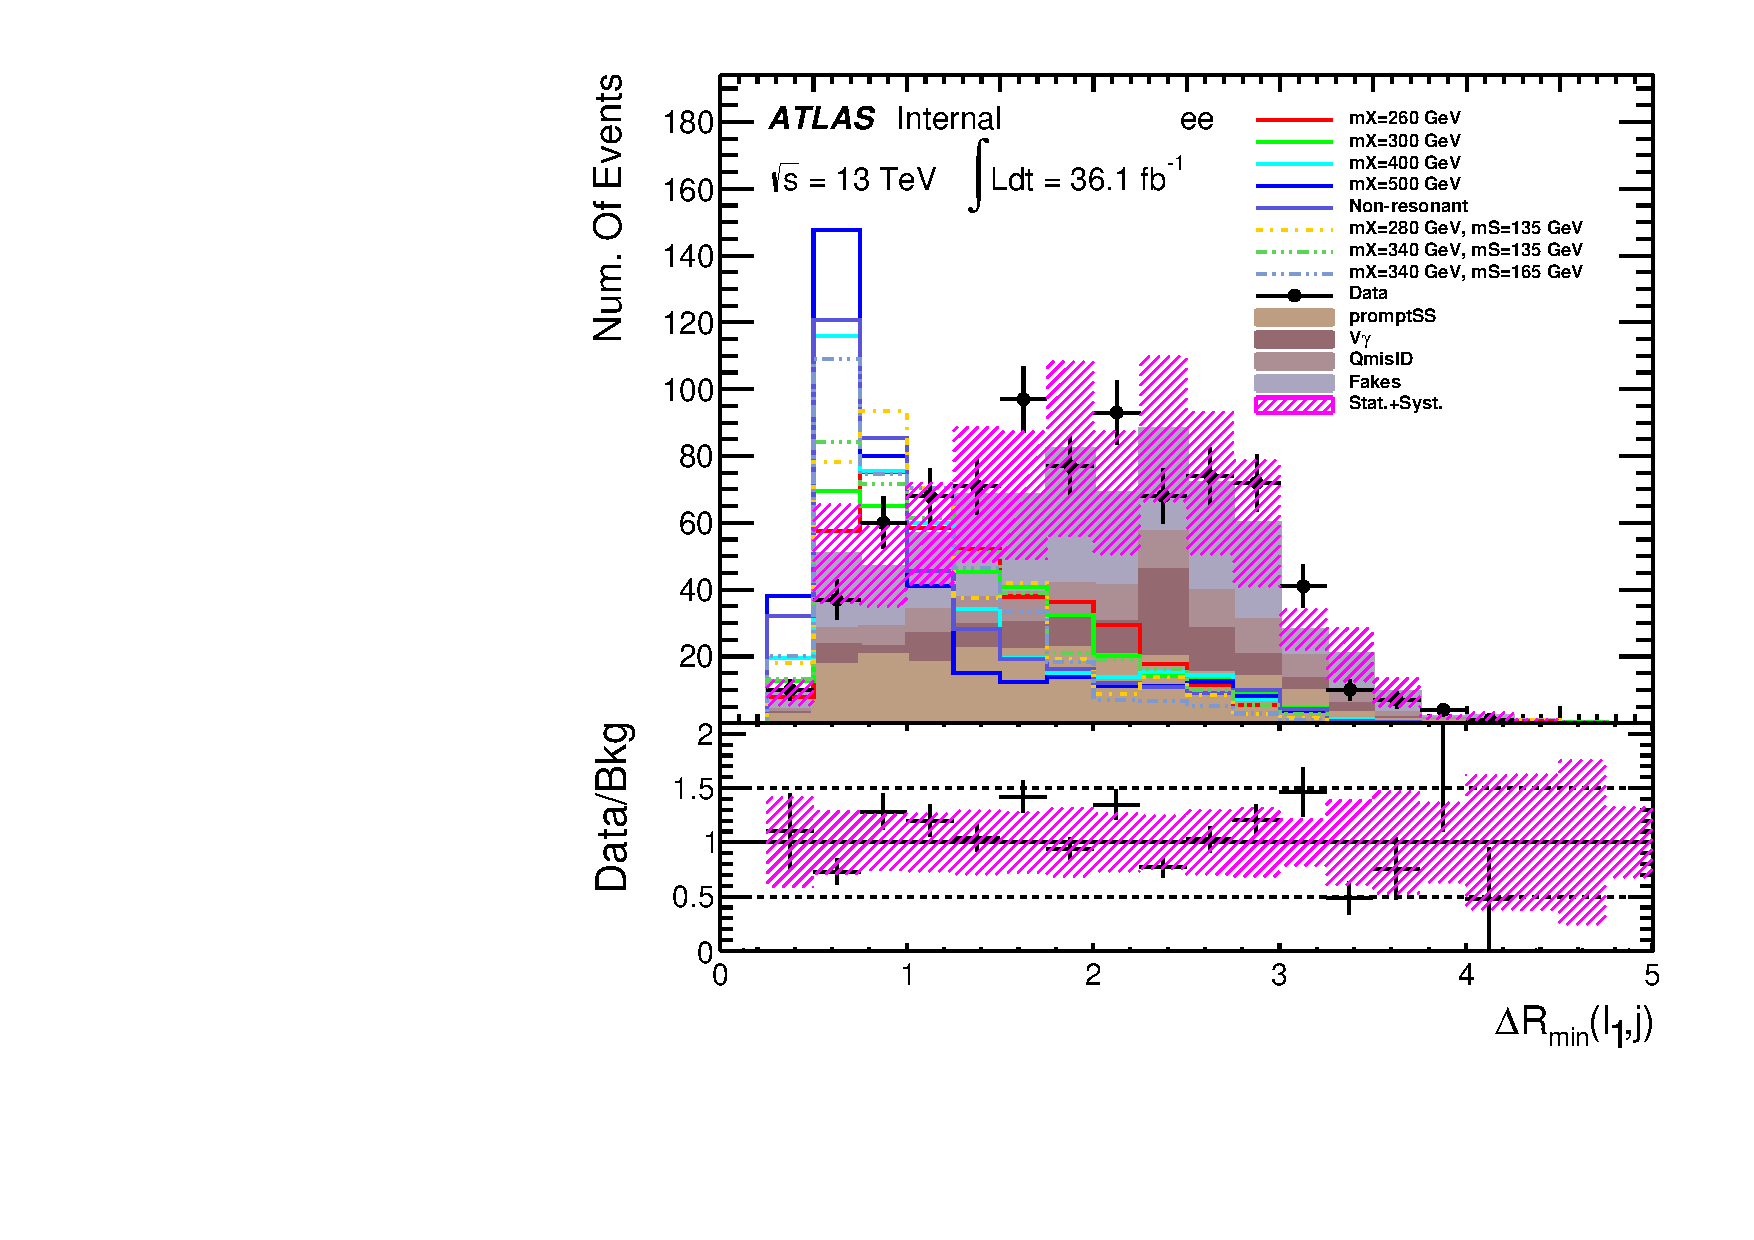
\includegraphics[width=0.9\textwidth,angle=-90]{fig/dataMC_low_Njet_CR/mindR_l1j_ee.pdf}\label{fig:dataMC_low_Njet_CR:mindRl1j_ee.pdf}
 \end{minipage}
 \begin{minipage}[t]{0.33\linewidth}
 \centering
 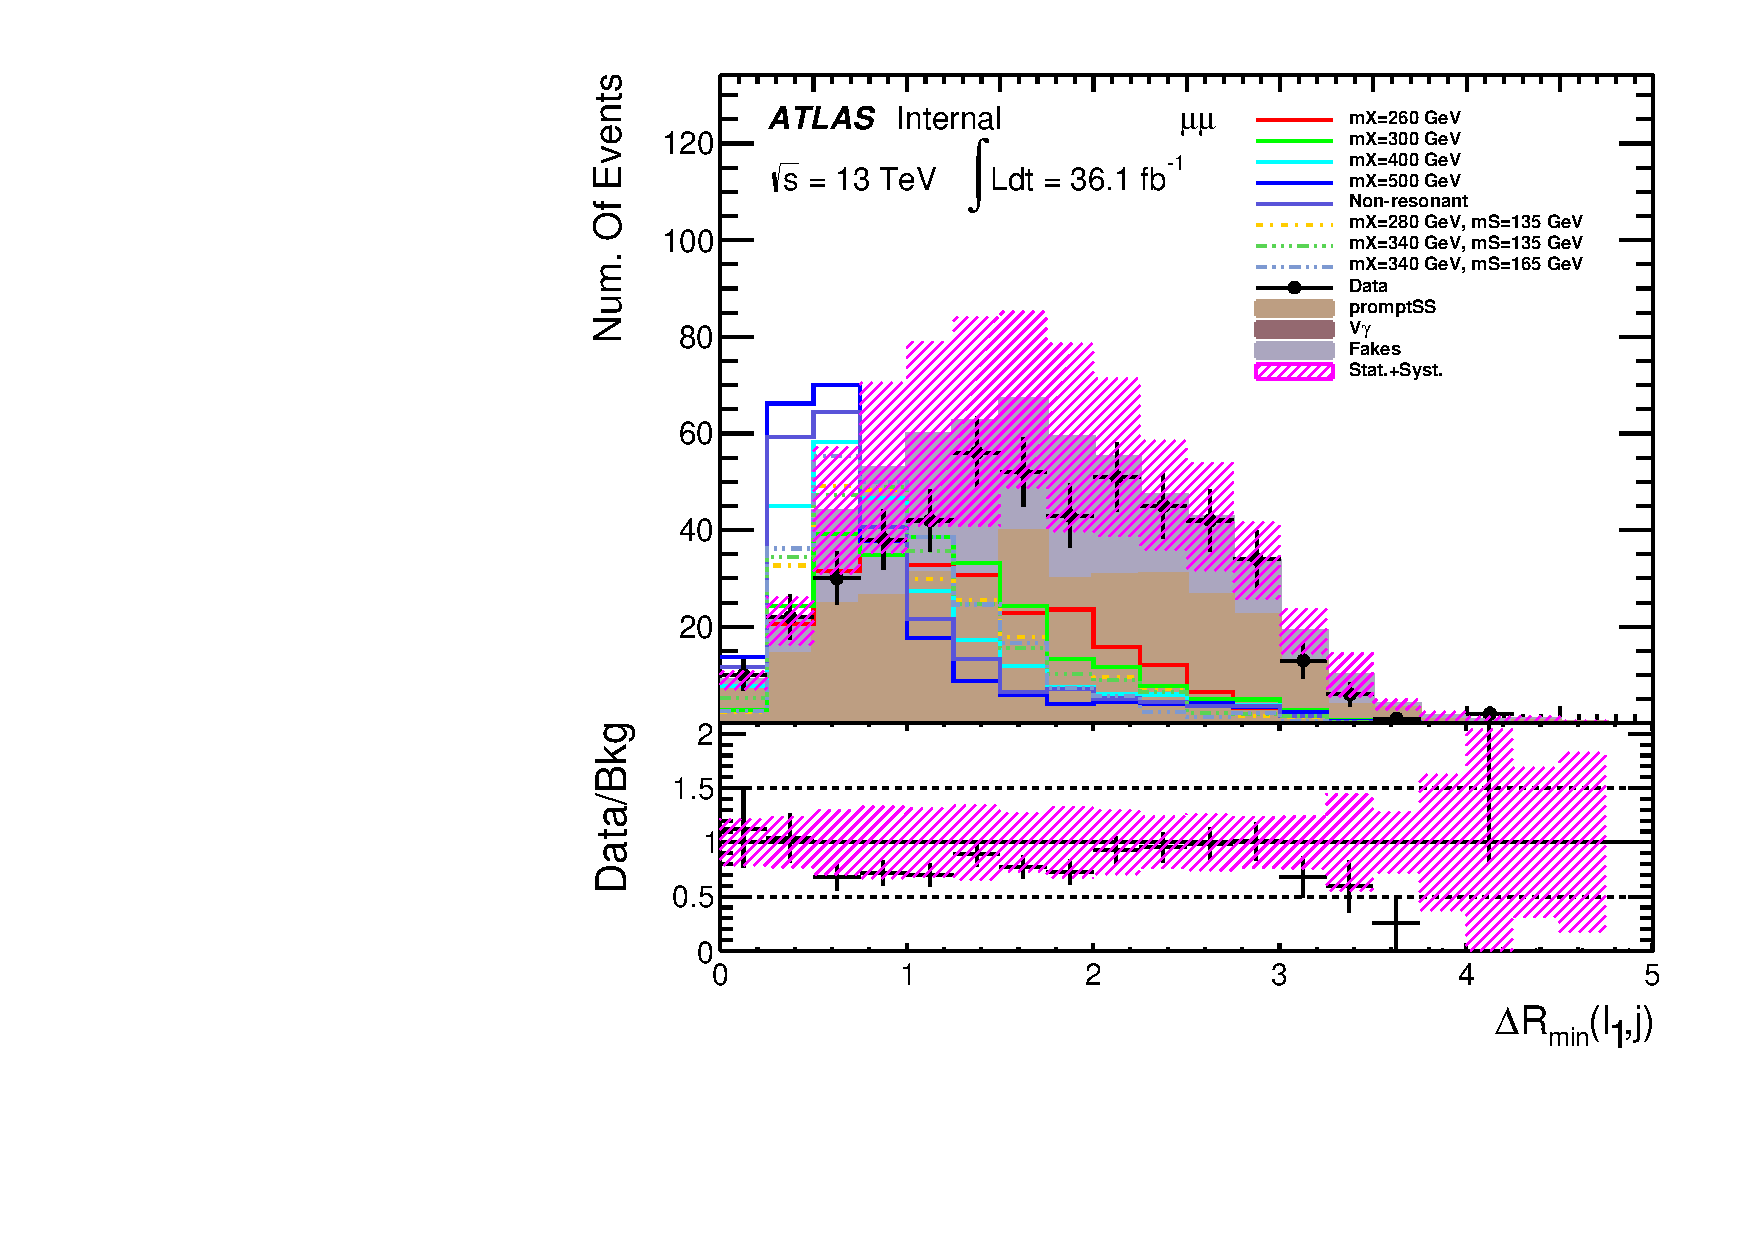
\includegraphics[width=0.9\textwidth,angle=-90]{fig/dataMC_low_Njet_CR/mindR_l1j_mumu.pdf}\label{fig:dataMC_low_Njet_CR:mindRl1j_mumu.pdf}
 \end{minipage}
 \begin{minipage}[t]{0.33\linewidth}
 \centering
 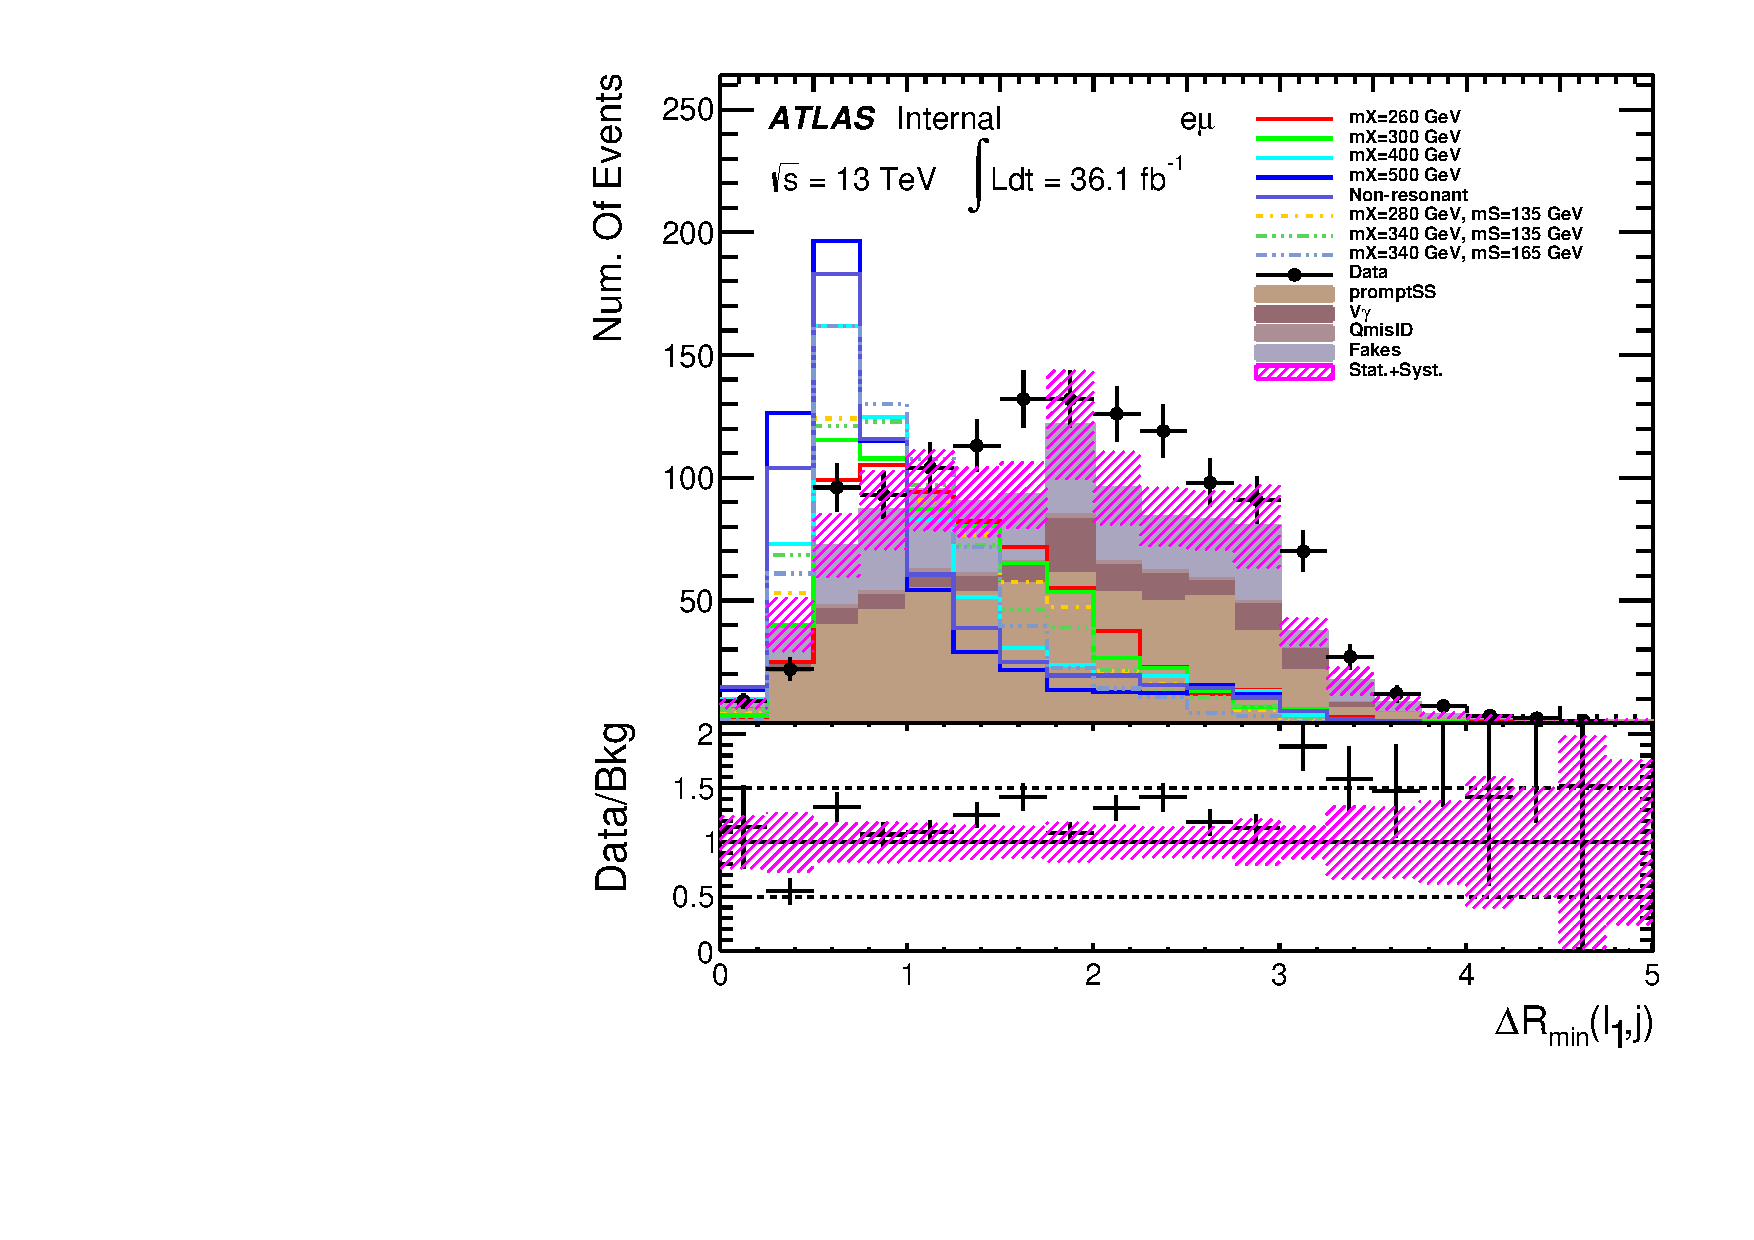
\includegraphics[width=0.9\textwidth,angle=-90]{fig/dataMC_low_Njet_CR/mindR_l1j_emu.pdf}\label{fig:dataMC_low_Njet_CR:mindRl1j_emu.pdf}
 \end{minipage}
 \begin{minipage}[t]{0.33\linewidth}
 \centering
 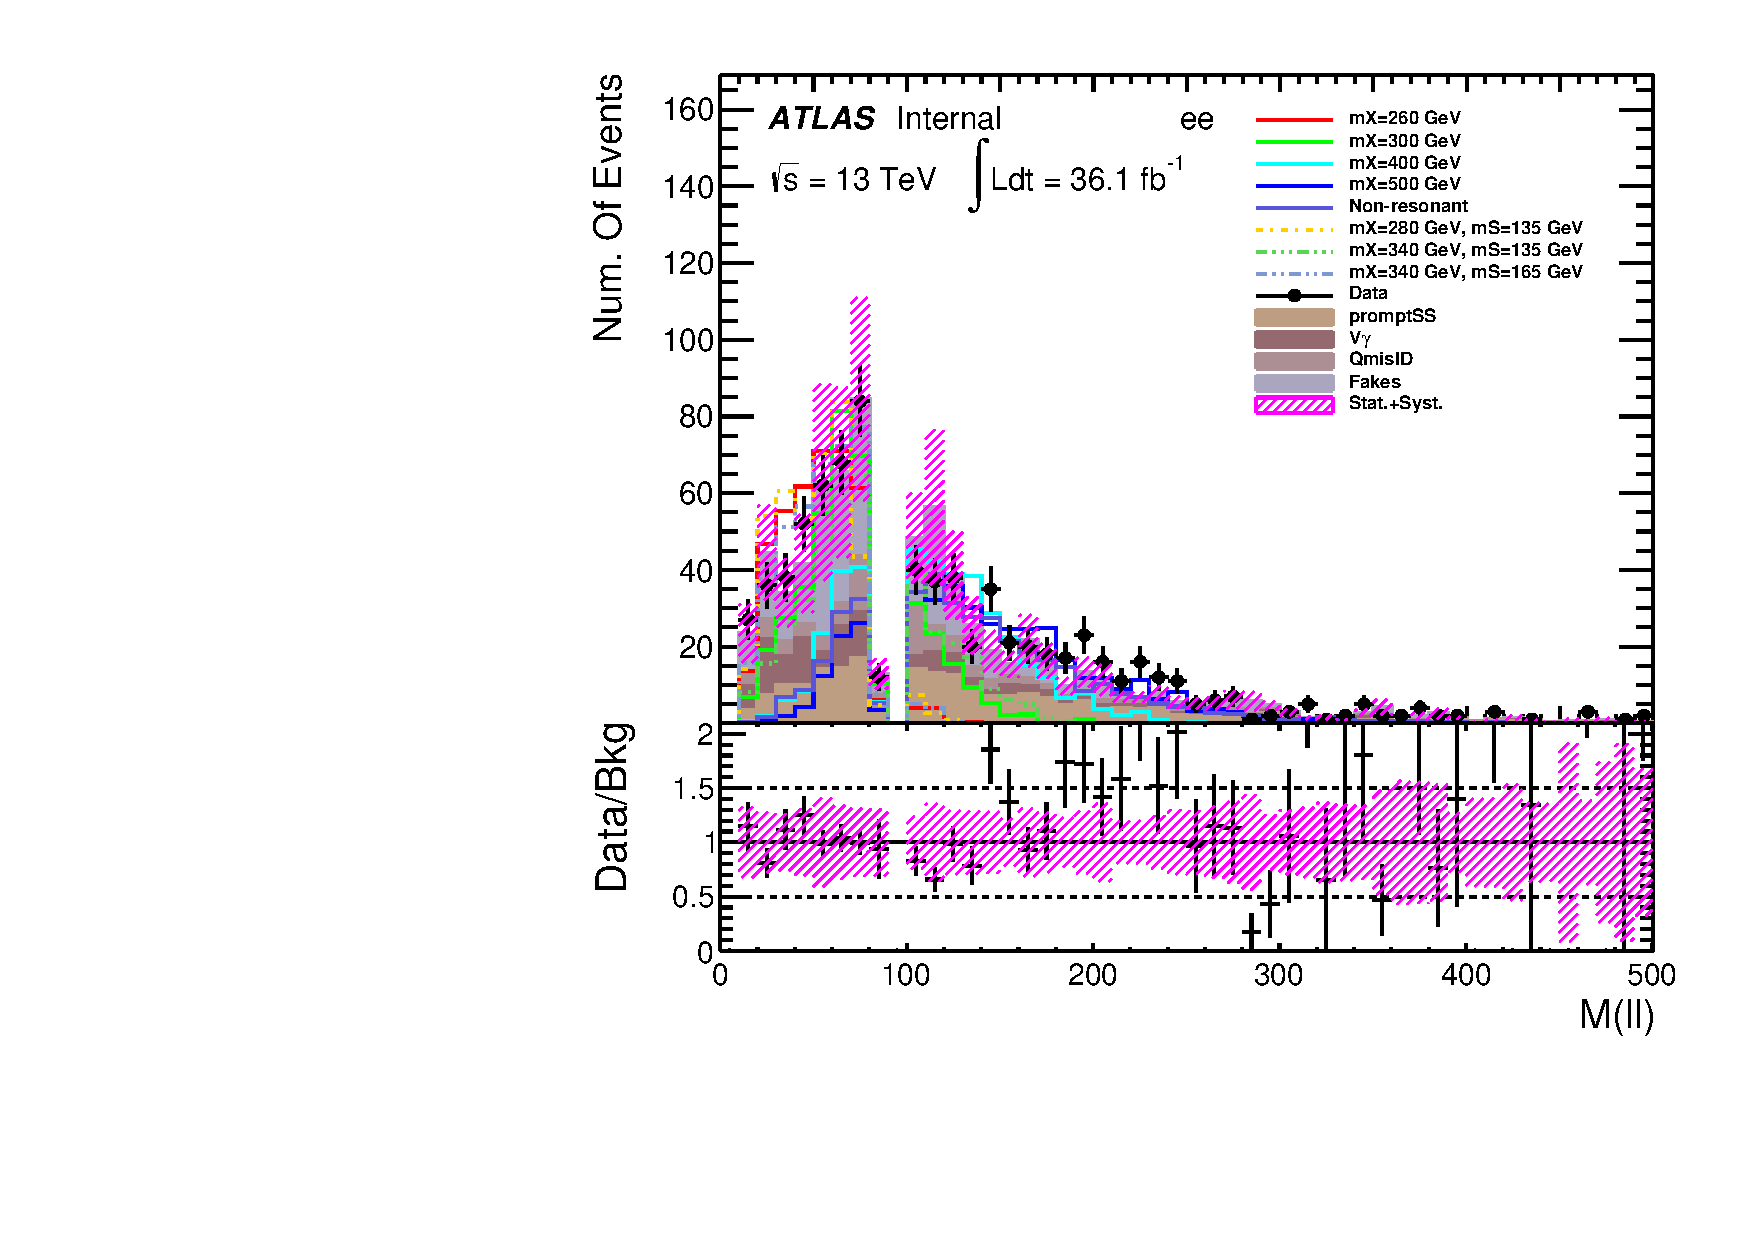
\includegraphics[width=0.9\textwidth,angle=-90]{fig/dataMC_low_Njet_CR/m_ll_ee.pdf}
 \label{fig:dataMC_low_Njet_CR:m_ll_ee.pdf}
 \end{minipage}
 \begin{minipage}[t]{0.33\linewidth}
 \centering
 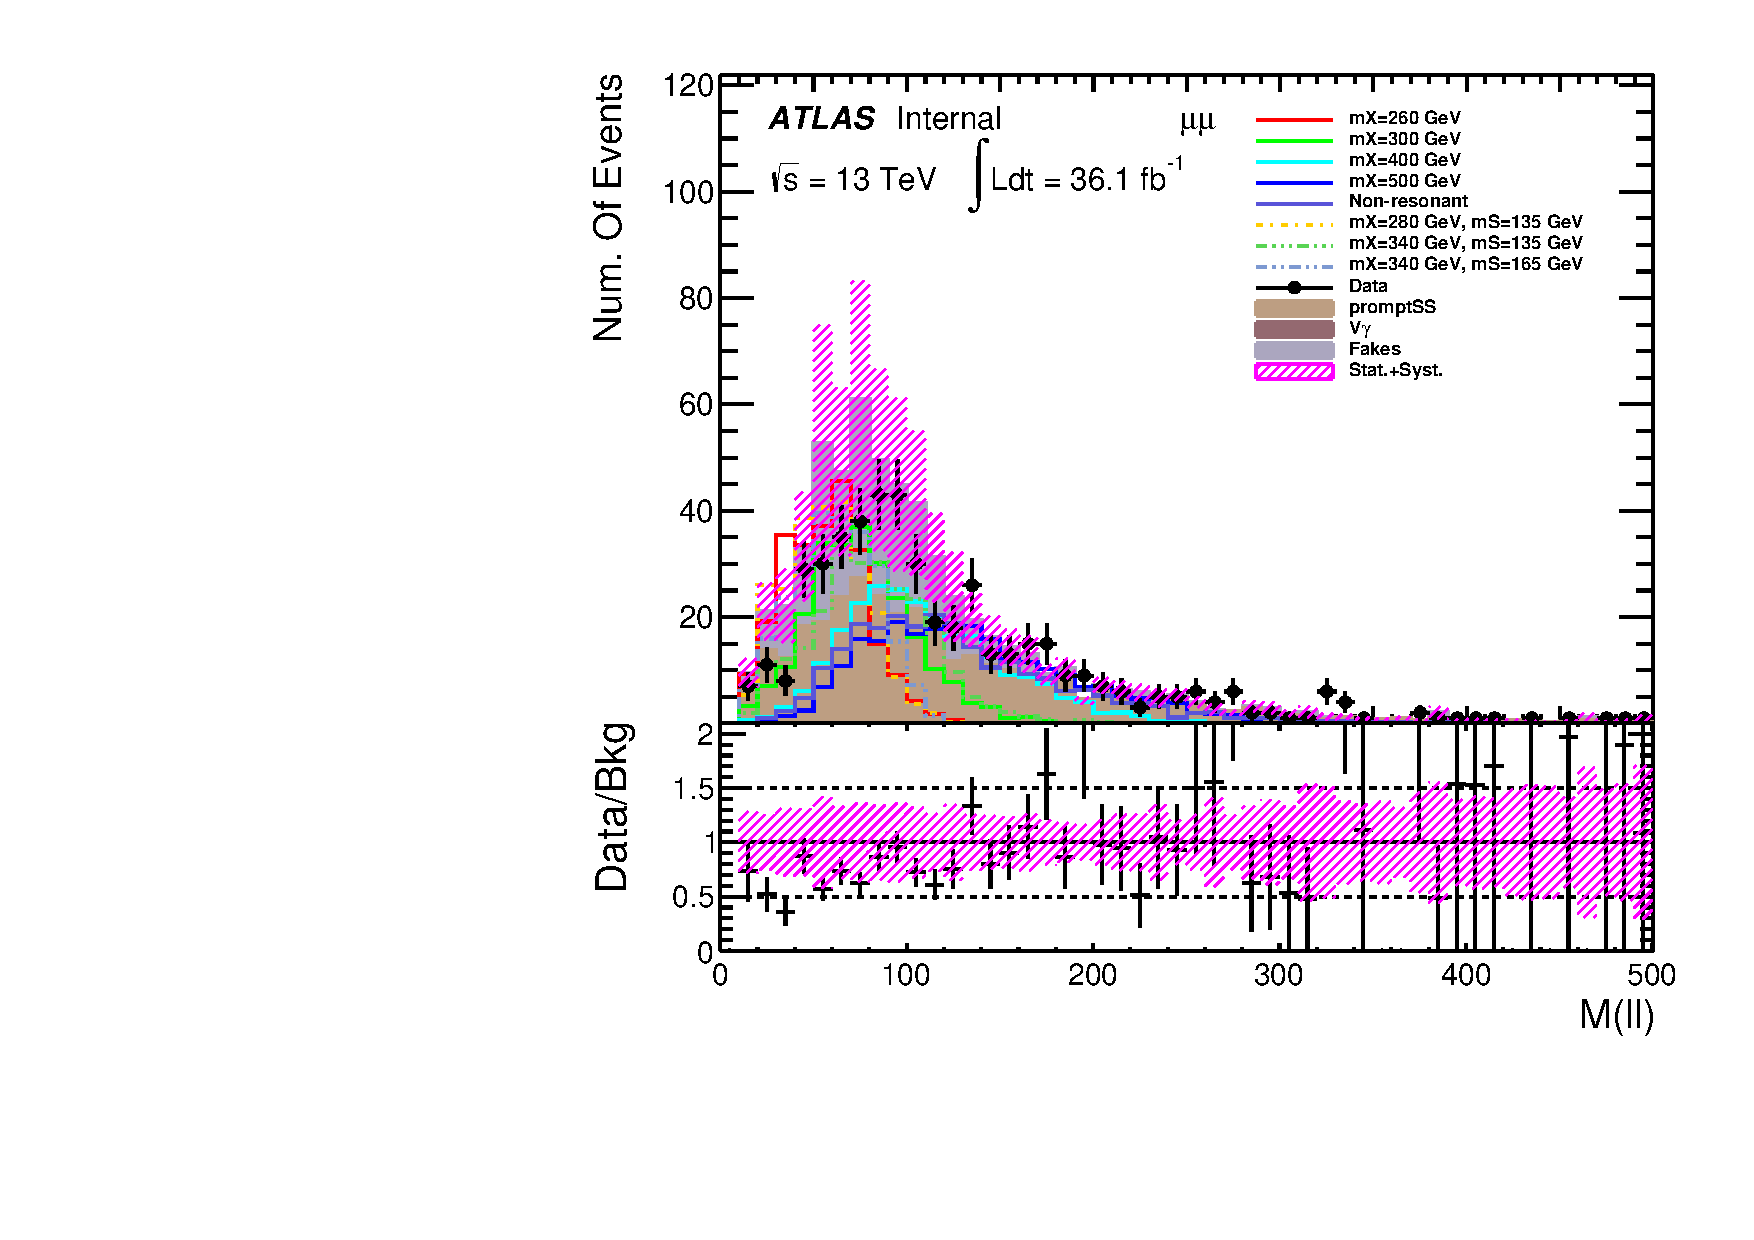
\includegraphics[width=0.9\textwidth,angle=-90]{fig/dataMC_low_Njet_CR/m_ll_mumu.pdf}
 \label{fig:dataMC_low_Njet_CR:m_ll_mumu.pdf}
 \end{minipage}
  \begin{minipage}[t]{0.33\linewidth}
 \centering
 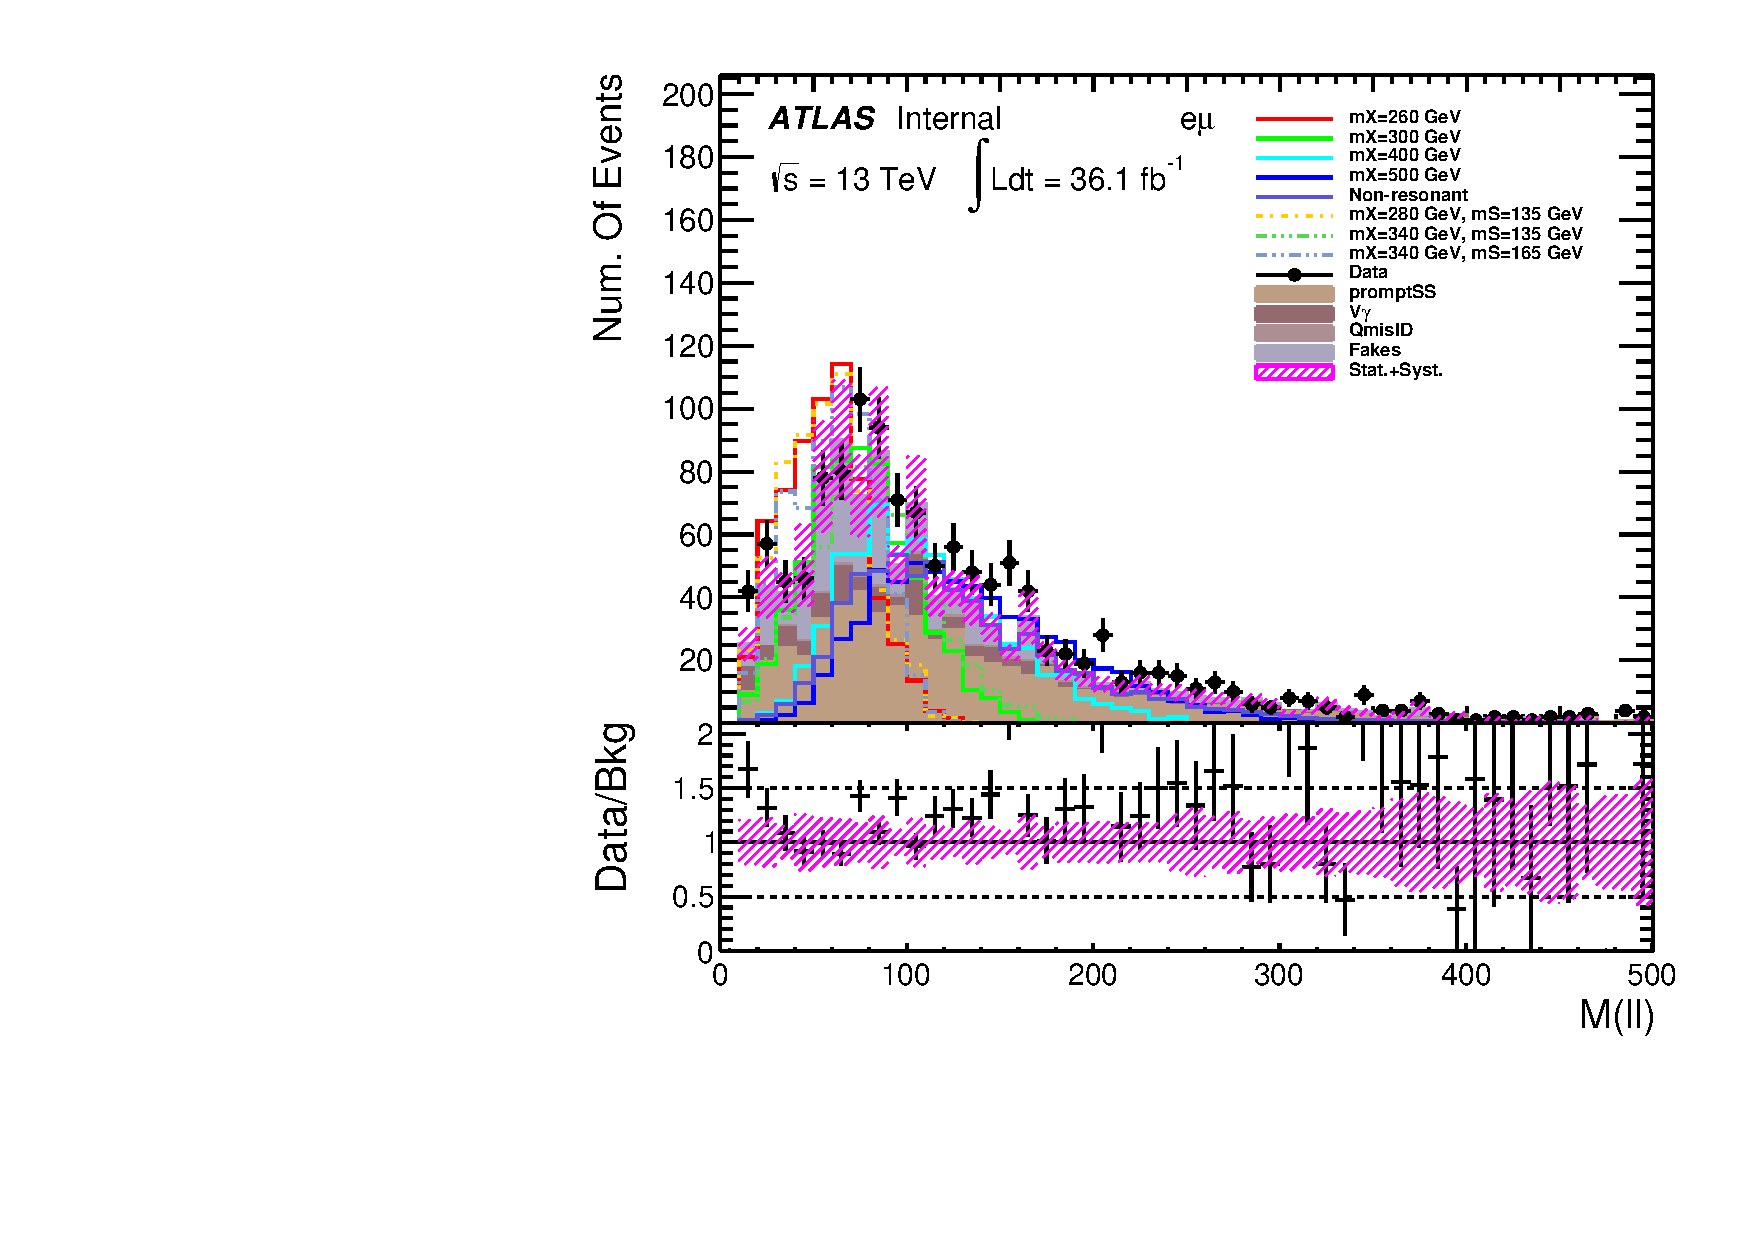
\includegraphics[width=0.9\textwidth,angle=-90]{fig/dataMC_low_Njet_CR/m_ll_emu.pdf}
 \label{fig:dataMC_low_Njet_CR:m_ll_emu.pdf}
 \end{minipage}
\begin{minipage}[t]{0.33\linewidth}
 \centering
 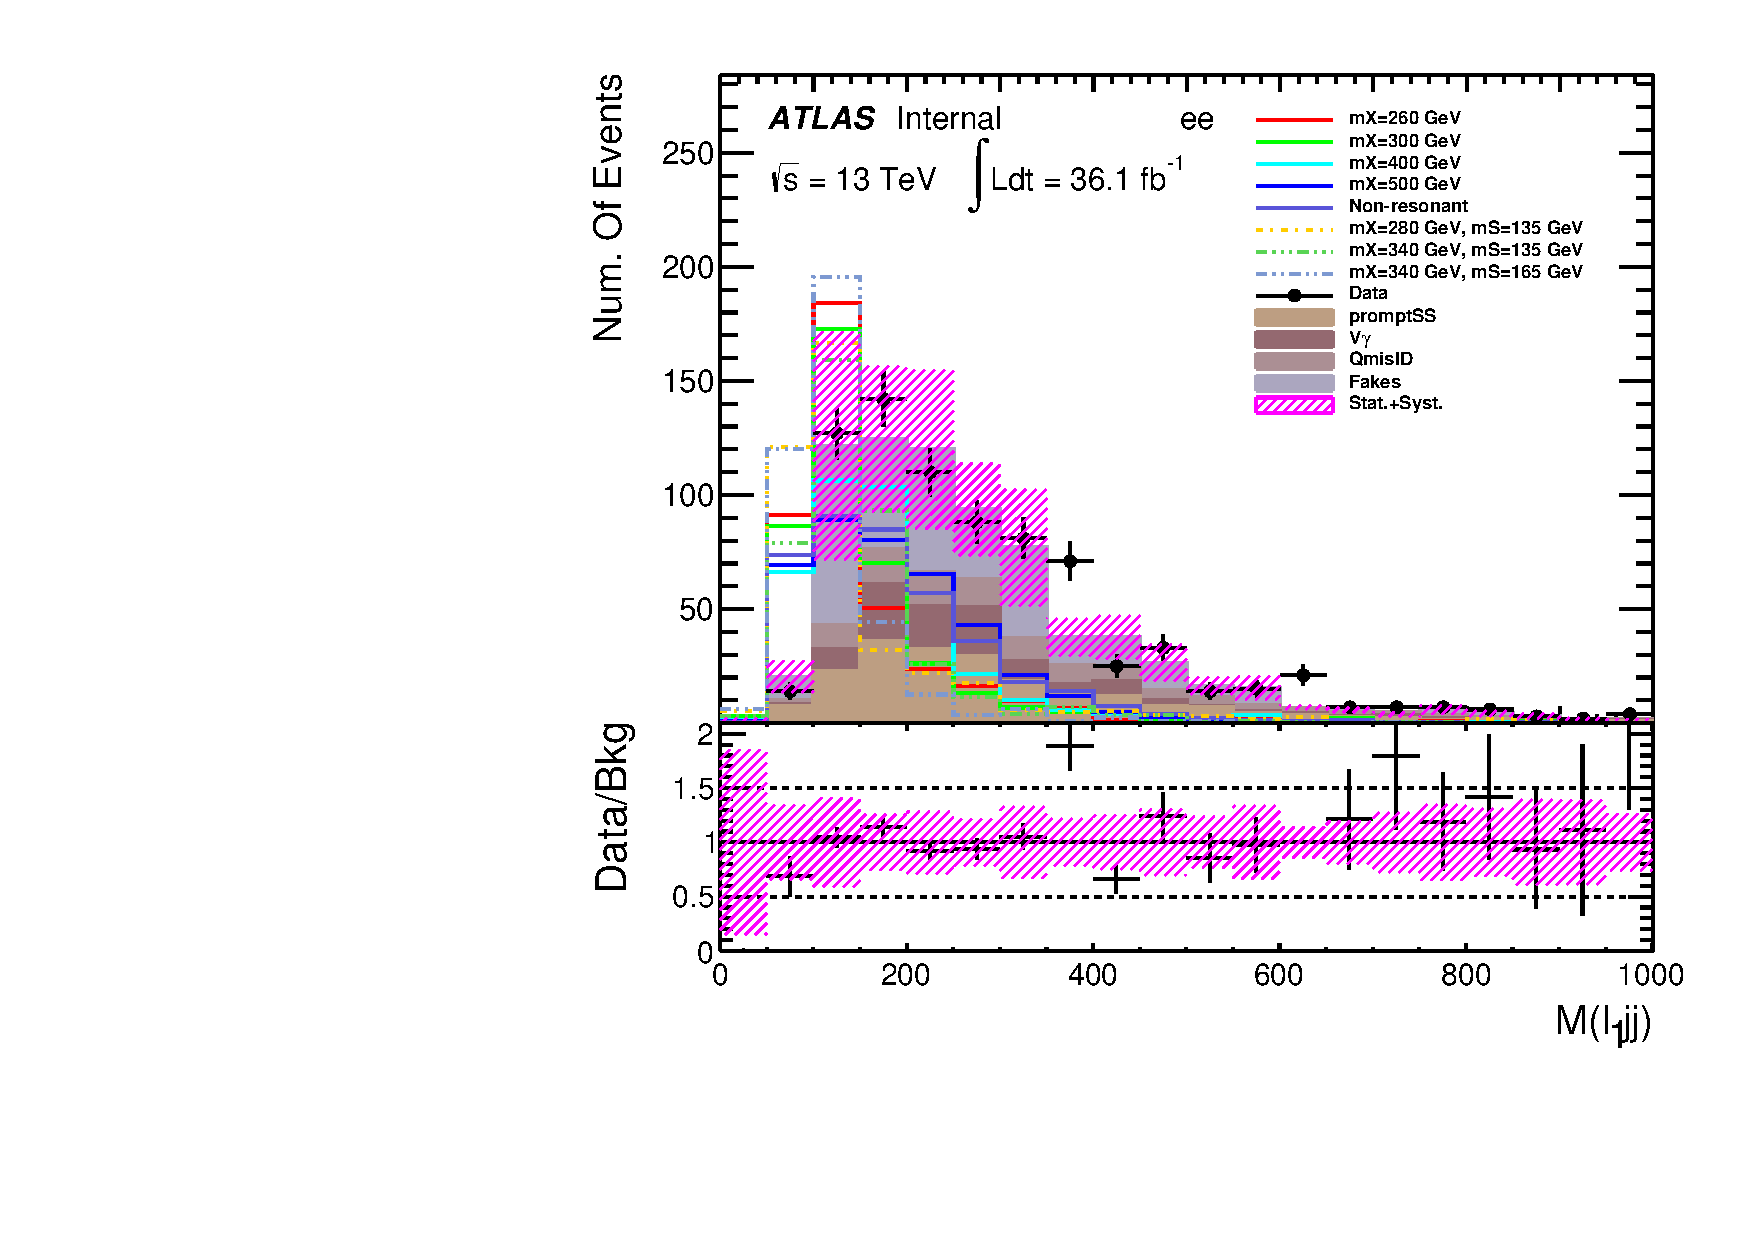
\includegraphics[width=0.9\textwidth,angle=-90]{fig/dataMC_low_Njet_CR/m_l1jj_ee.pdf}\label{fig:dataMC_low_Njet_CR:m_l1jj_ee.pdf}
 \end{minipage}
 \begin{minipage}[t]{0.33\linewidth}
 \centering
 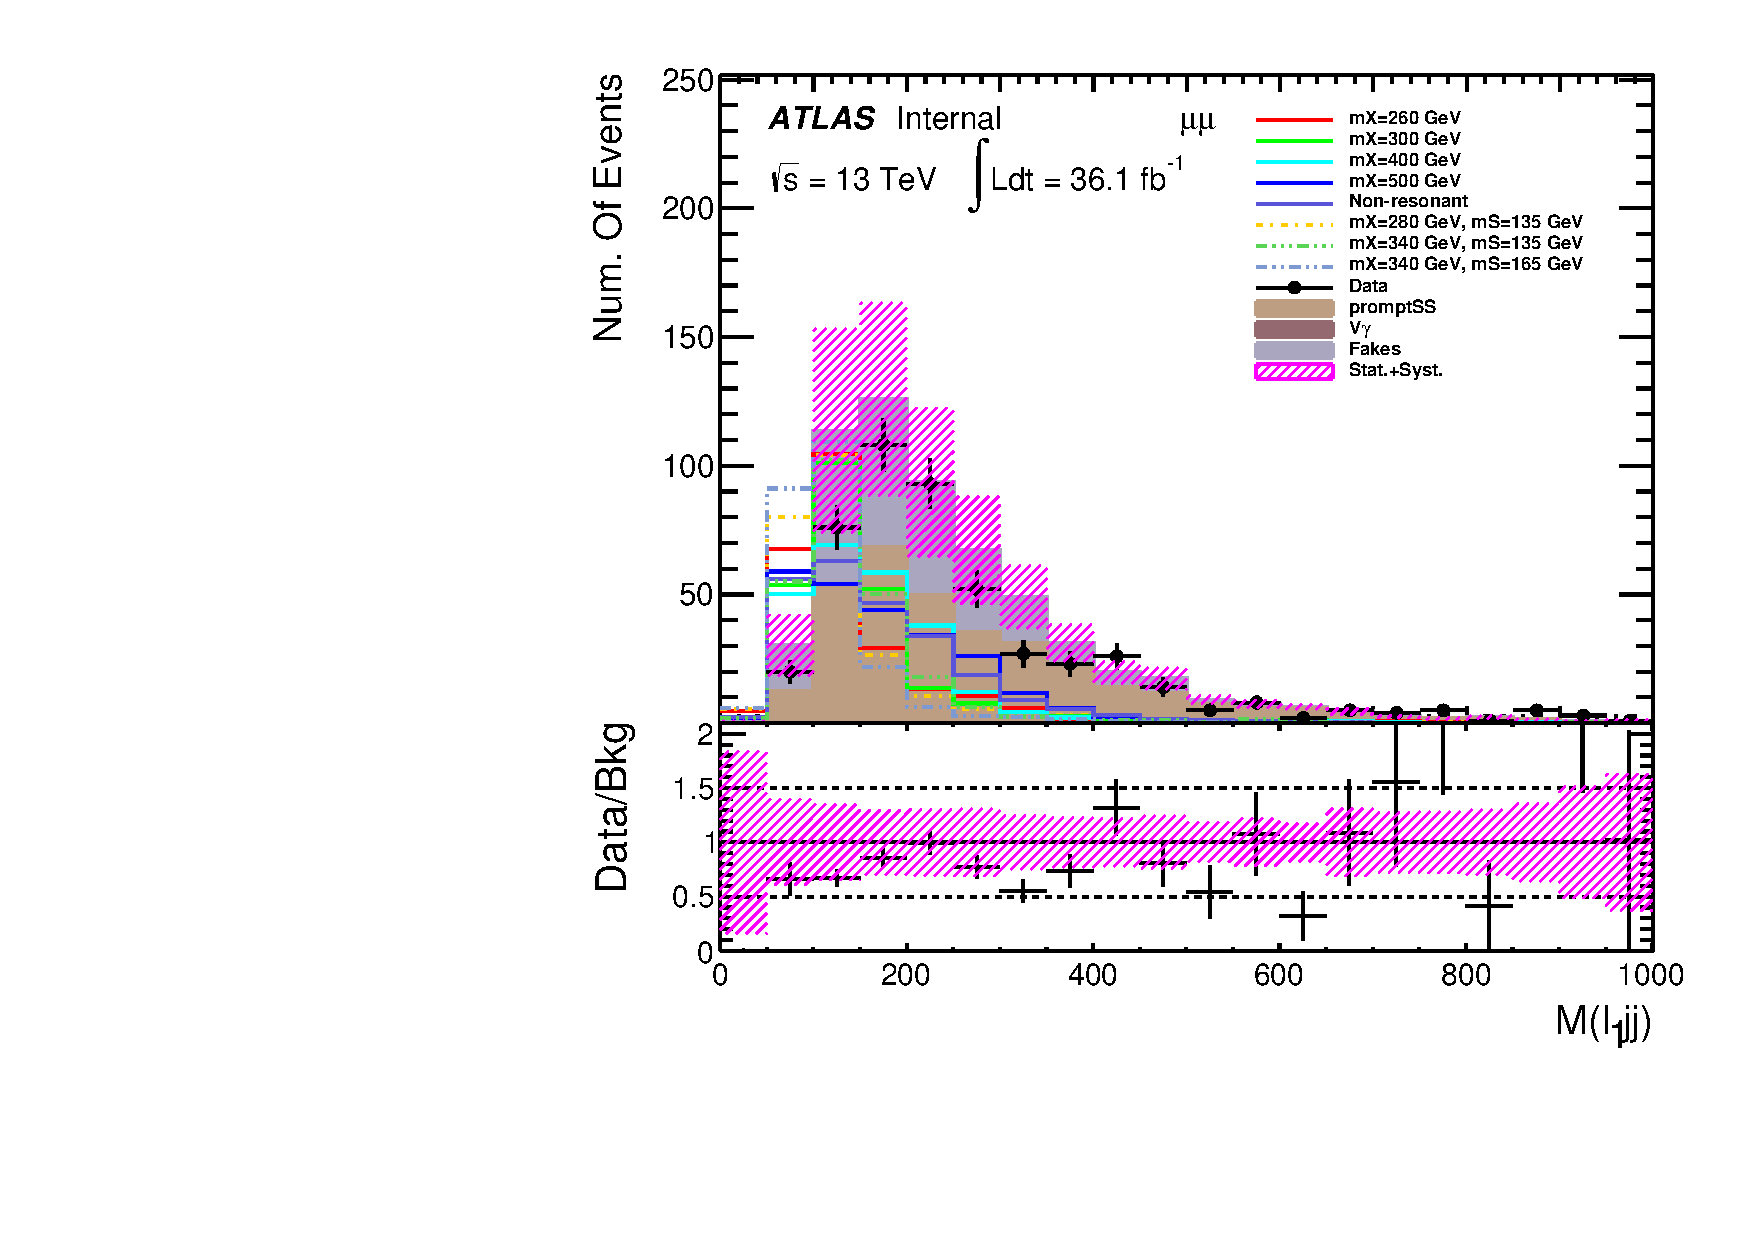
\includegraphics[width=0.9\textwidth,angle=-90]{fig/dataMC_low_Njet_CR/m_l1jj_mumu.pdf}\label{fig:dataMC_low_Njet_CR:m_l1jj_mumu.pdf}
 \end{minipage}
 \begin{minipage}[t]{0.33\linewidth}
 \centering
 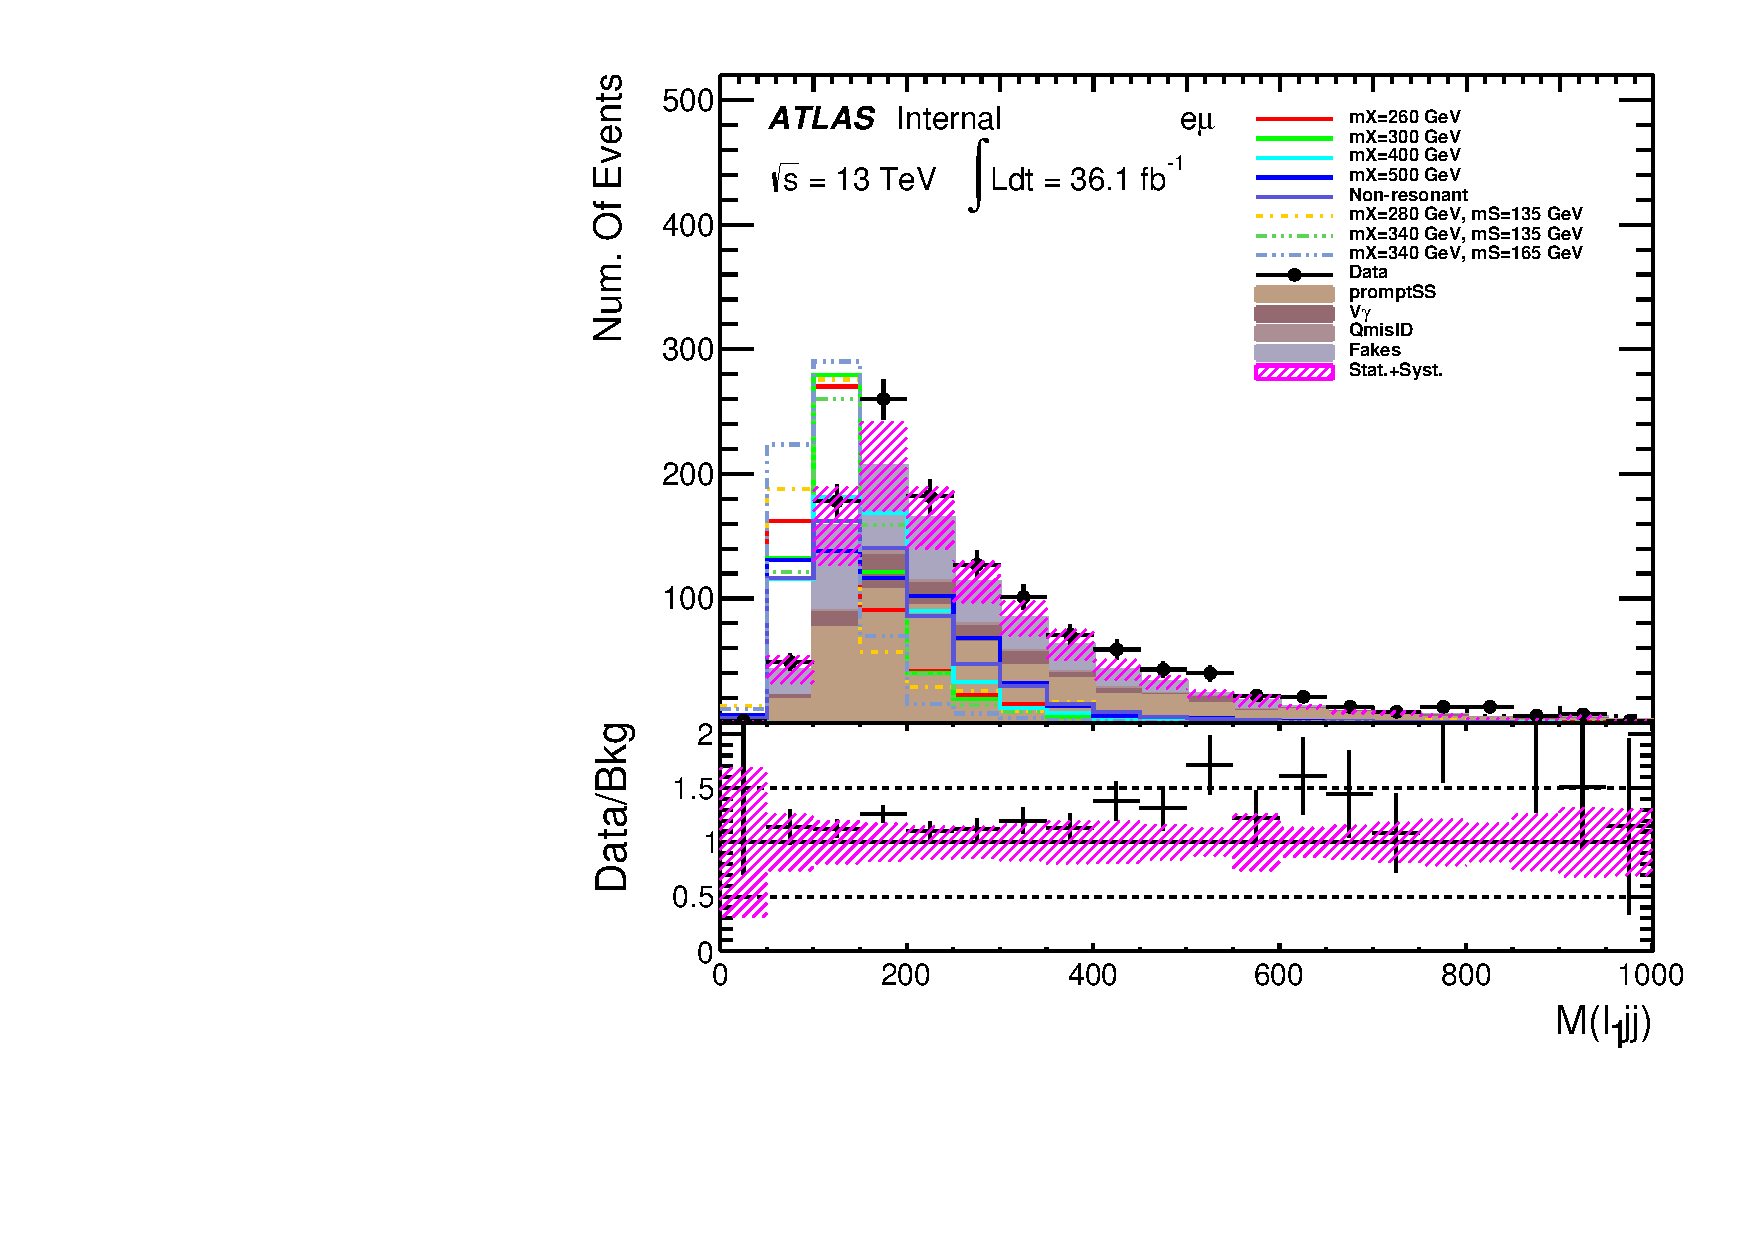
\includegraphics[width=0.9\textwidth,angle=-90]{fig/dataMC_low_Njet_CR/m_l1jj_emu.pdf}\label{fig:dataMC_low_Njet_CR:m_l1jj_emu.pdf}
 \end{minipage}
 \begin{minipage}[t]{0.33\linewidth}
 \centering
 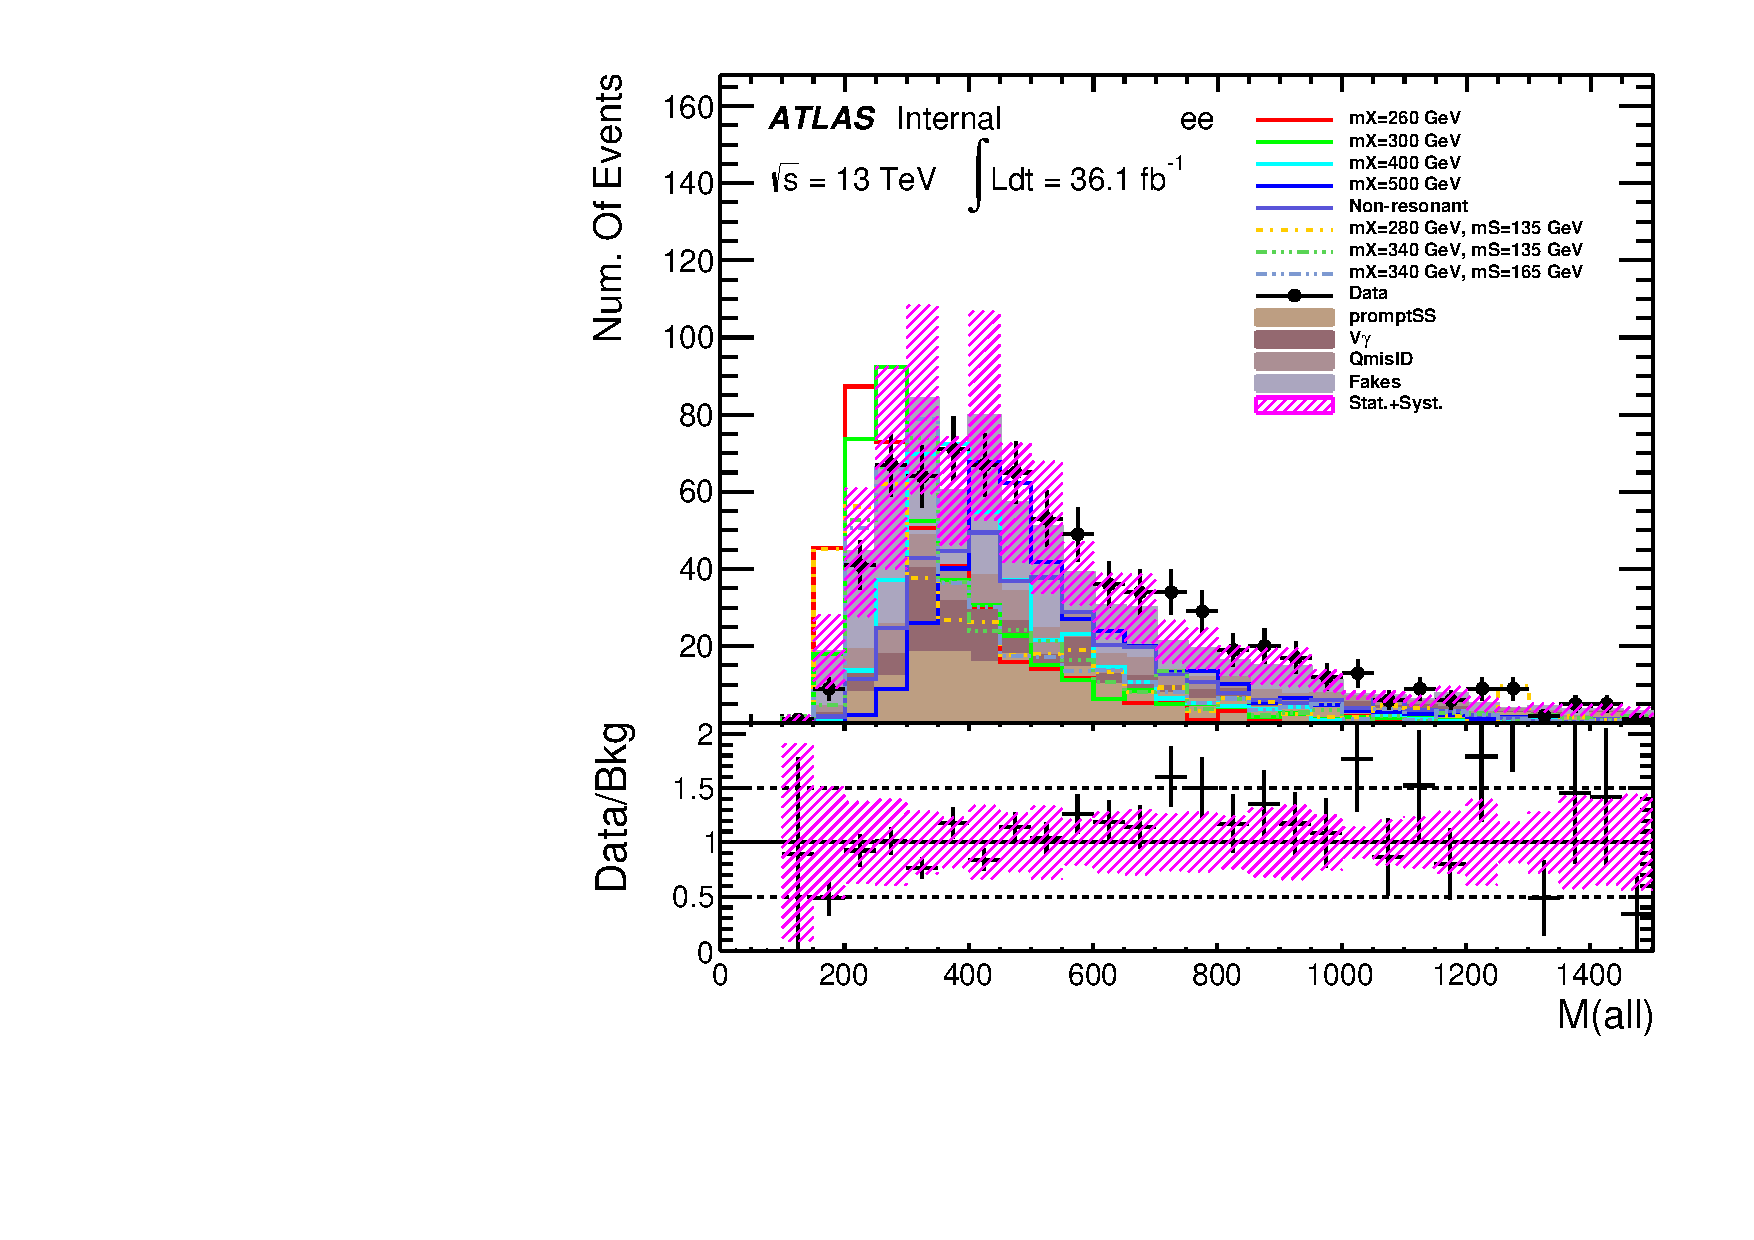
\includegraphics[width=0.9\textwidth,angle=-90]{fig/dataMC_low_Njet_CR/m_all_ee.pdf}\label{fig:dataMC_low_Njet_CR:m_all_ee.pdf}
 \end{minipage}
  \begin{minipage}[t]{0.33\linewidth}
 \centering
 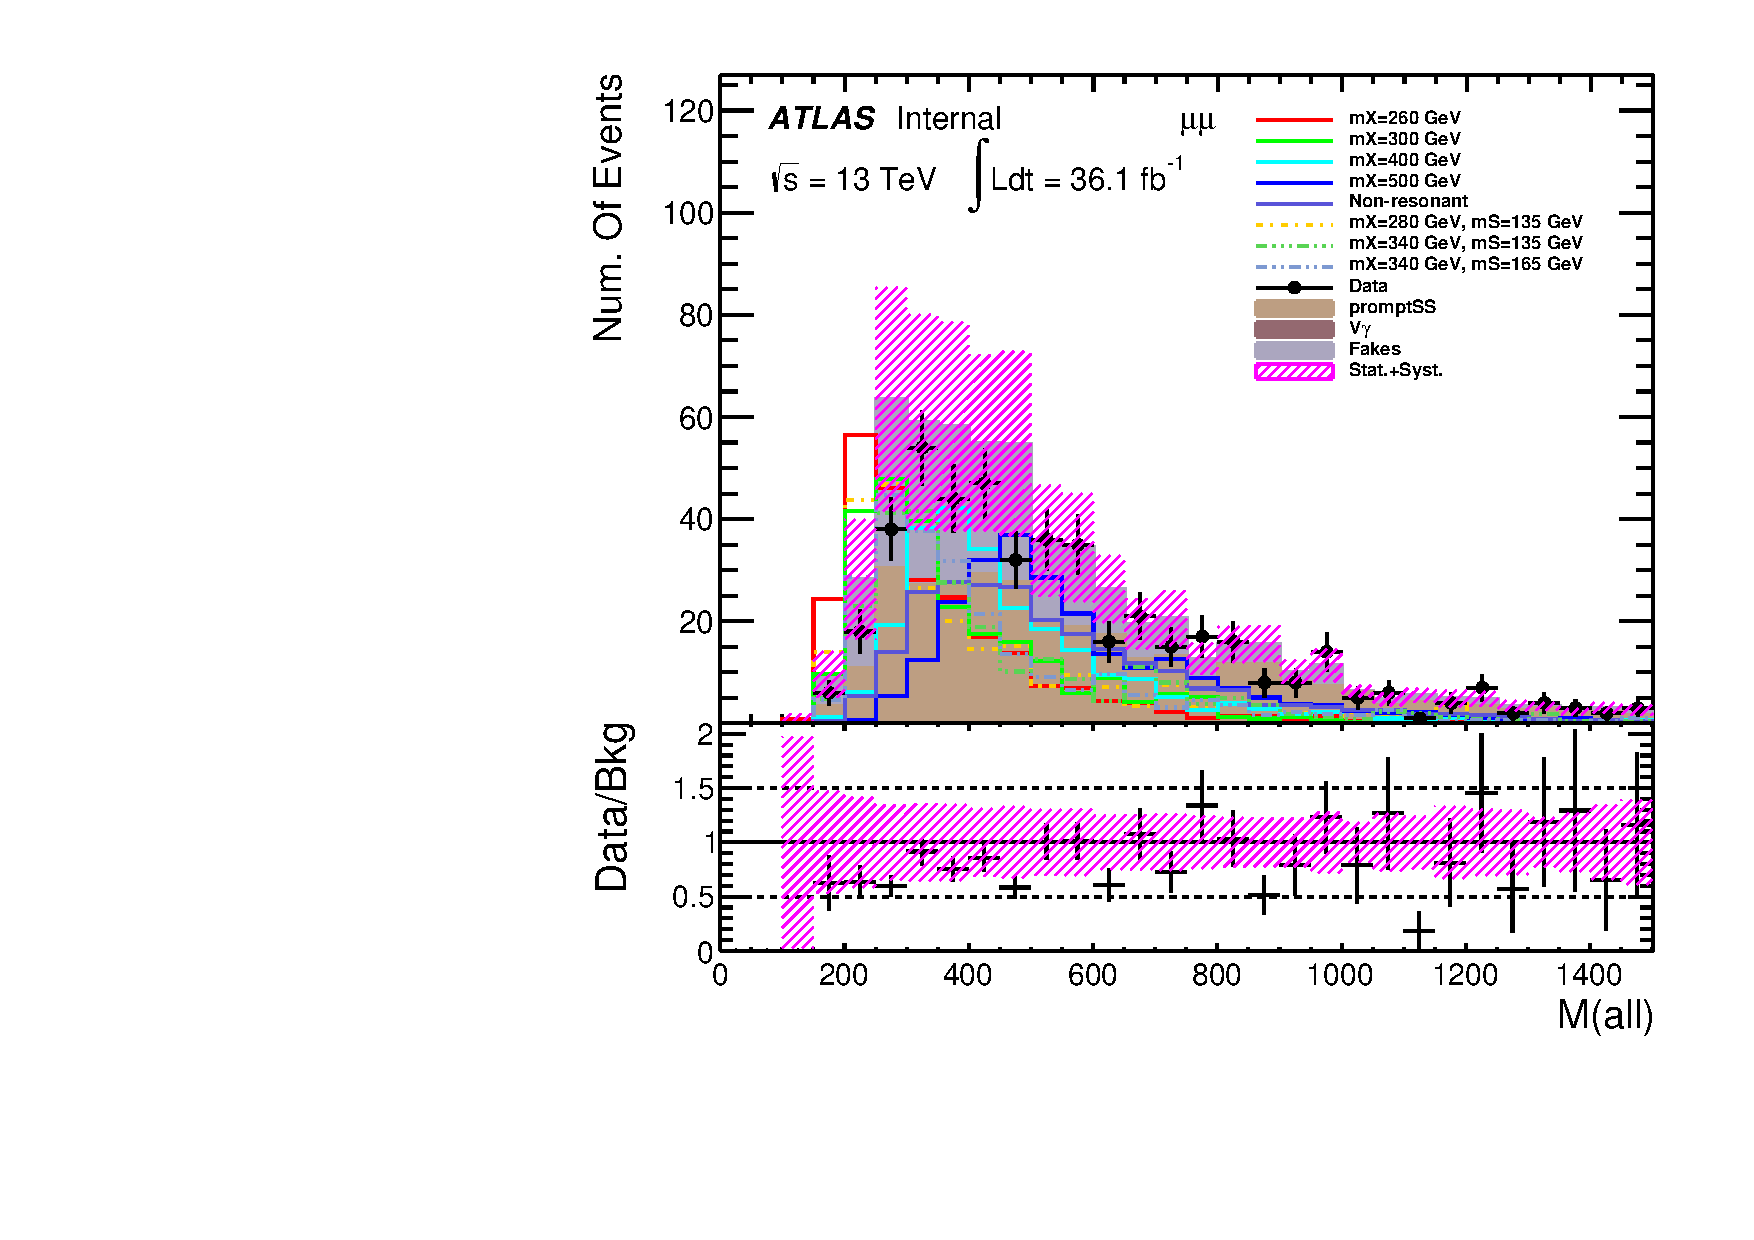
\includegraphics[width=0.9\textwidth,angle=-90]{fig/dataMC_low_Njet_CR/m_all_mumu.pdf}\label{fig:dataMC_low_Njet_CR:m_all_mumu.pdf}
 \end{minipage}
 \begin{minipage}[t]{0.33\linewidth}
 \centering
 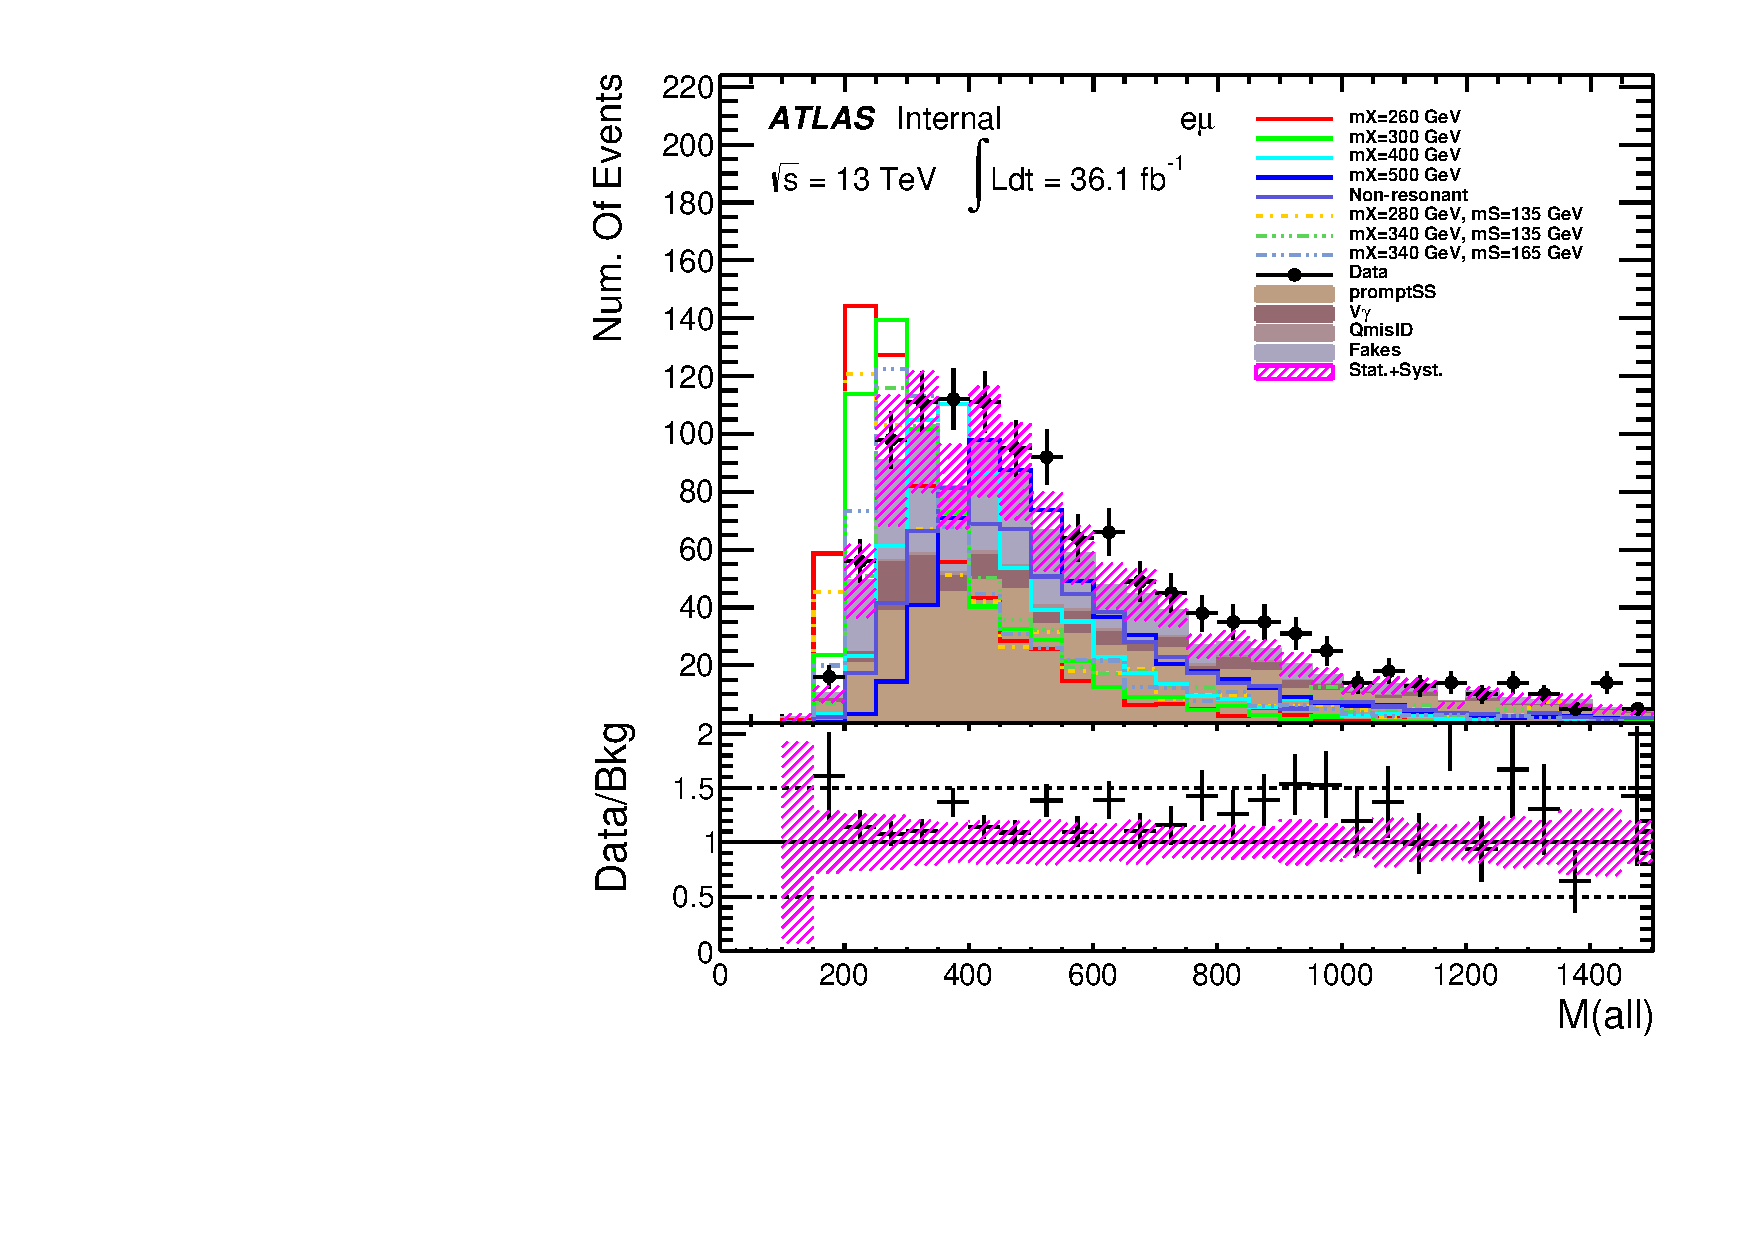
\includegraphics[width=0.9\textwidth,angle=-90]{fig/dataMC_low_Njet_CR/m_all_emu.pdf}\label{fig:dataMC_low_Njet_CR:m_all_emu.pdf}
 \end{minipage}
 \caption{用于低质量信号优化的运动学变量分布,对应$N_{\text{jet}}\geq2$。}
 %\caption{The distributions of kinematic variables that are used to form optimization selections at pre-selection level, corresponding to $N_{\text{jet}}\geq2$. Left: $ee$, middle: $\mu\mu$, right: $e\mu$. PromptSS and $V+\gamma$ are normalized to the luminosity of 36.1 fb$^{-1}$.}
\label{fig:SigOpt_low_kine}
\end{figure}

\begin{figure}[h]
 \begin{minipage}[t]{0.33\linewidth}
 \centering
 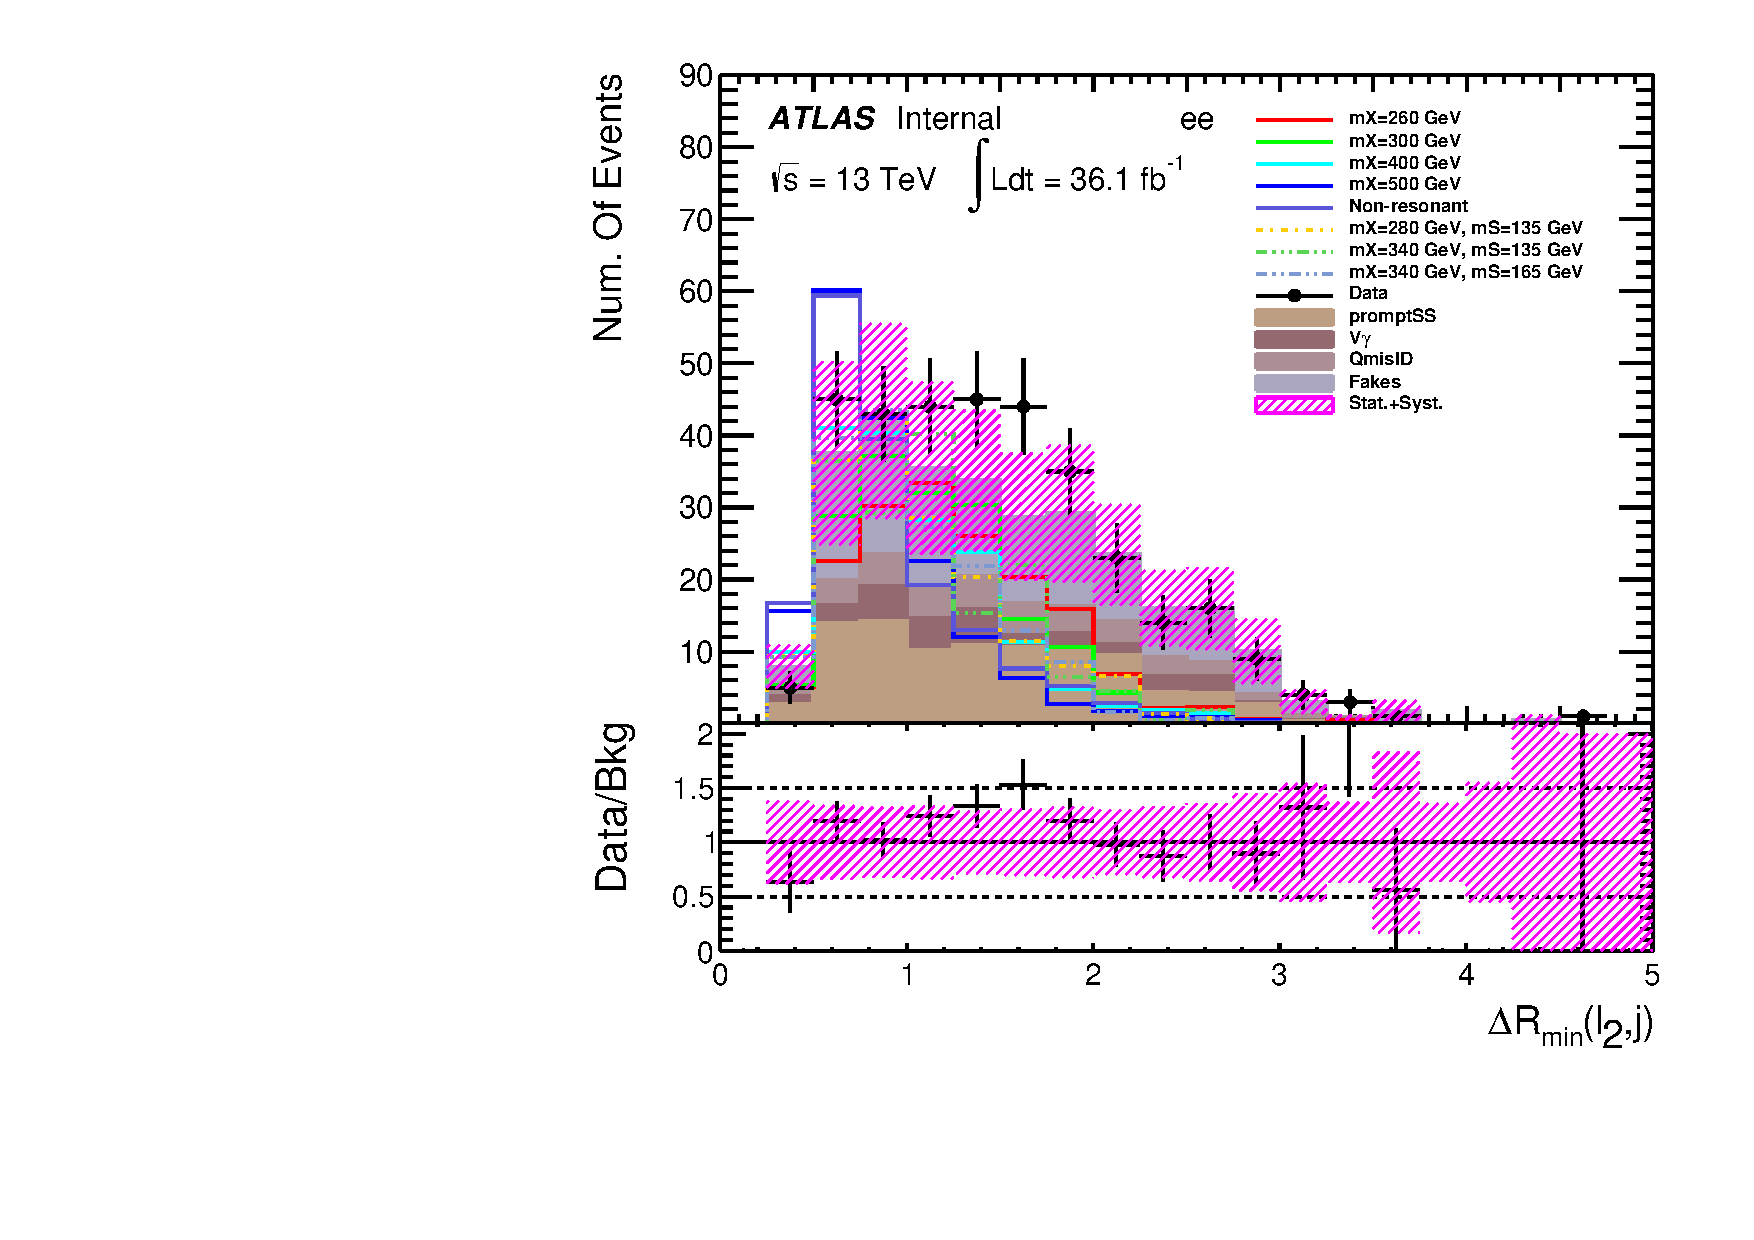
\includegraphics[width=0.9\textwidth,angle=-90]{fig/dataMC_high_Njet_CR/mindR_l2j_ee.pdf}\label{fig:dataMC_high_Njet_CR:mindRl2j_ee.pdf}
 \end{minipage}
 \begin{minipage}[t]{0.33\linewidth}
 \centering
 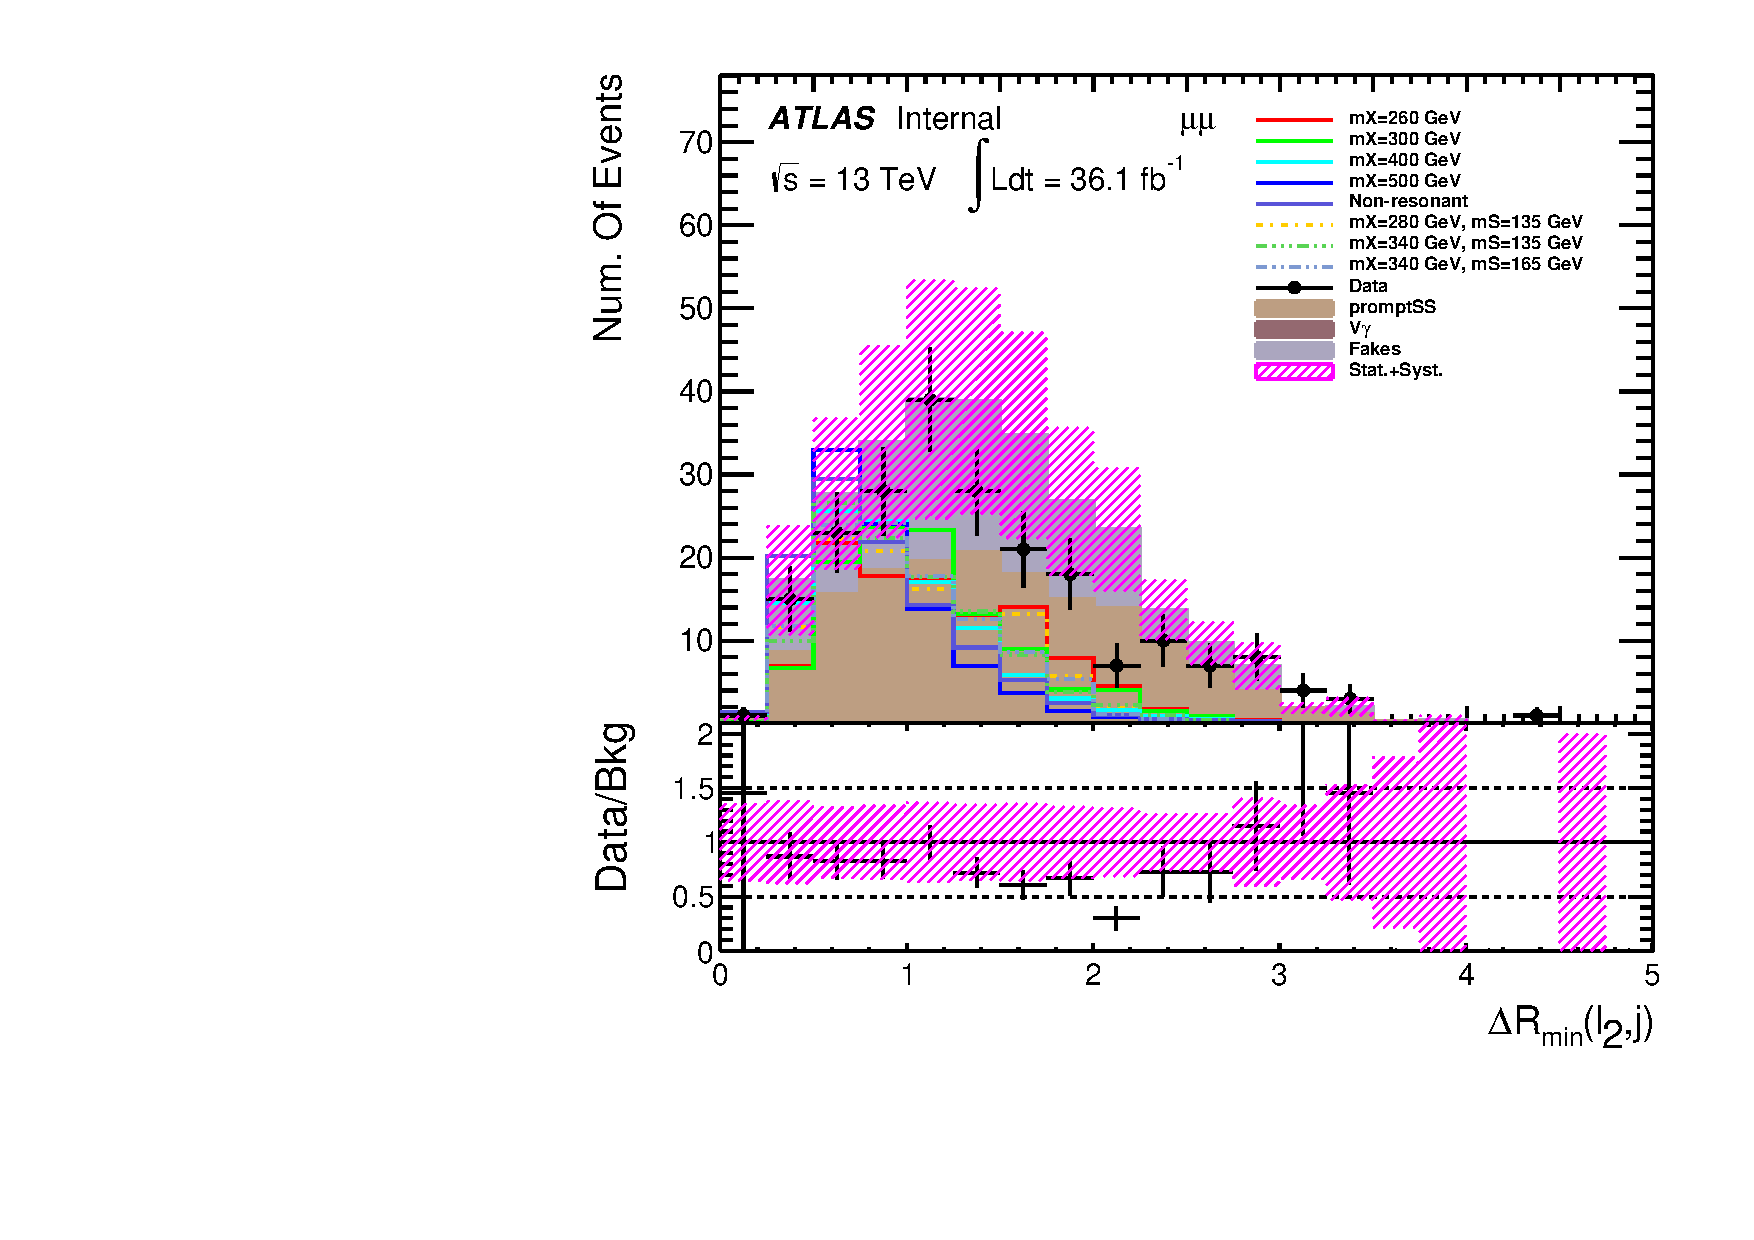
\includegraphics[width=0.9\textwidth,angle=-90]{fig/dataMC_high_Njet_CR/mindR_l2j_mumu.pdf}\label{fig:dataMC_high_Njet_CR:mindRl2j_mumu.pdf}
 \end{minipage}
 \begin{minipage}[t]{0.33\linewidth}
 \centering
 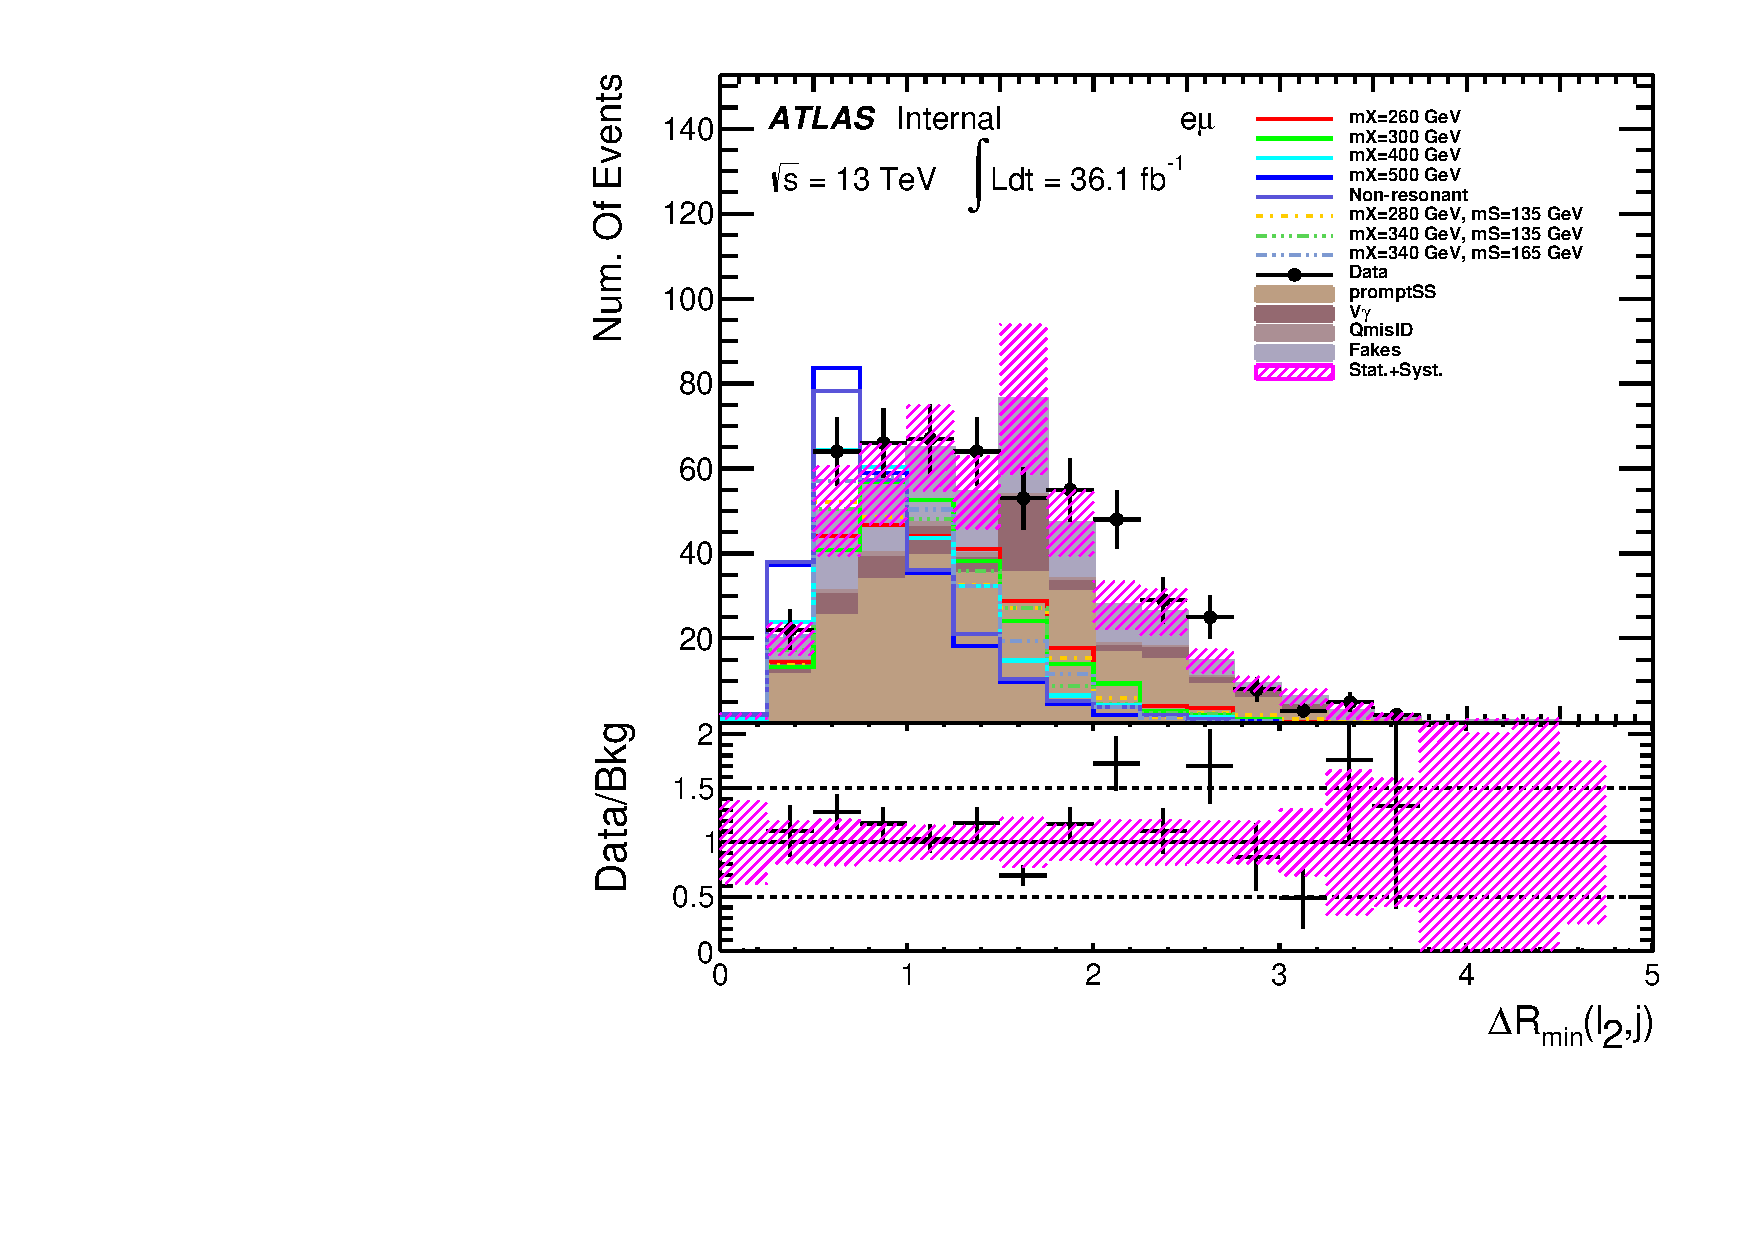
\includegraphics[width=0.9\textwidth,angle=-90]{fig/dataMC_high_Njet_CR/mindR_l2j_emu.pdf}\label{fig:dataMC_high_Njet_CR:mindRl2j_emu.pdf}
 \end{minipage}
 \begin{minipage}[t]{0.33\linewidth}
 \centering
 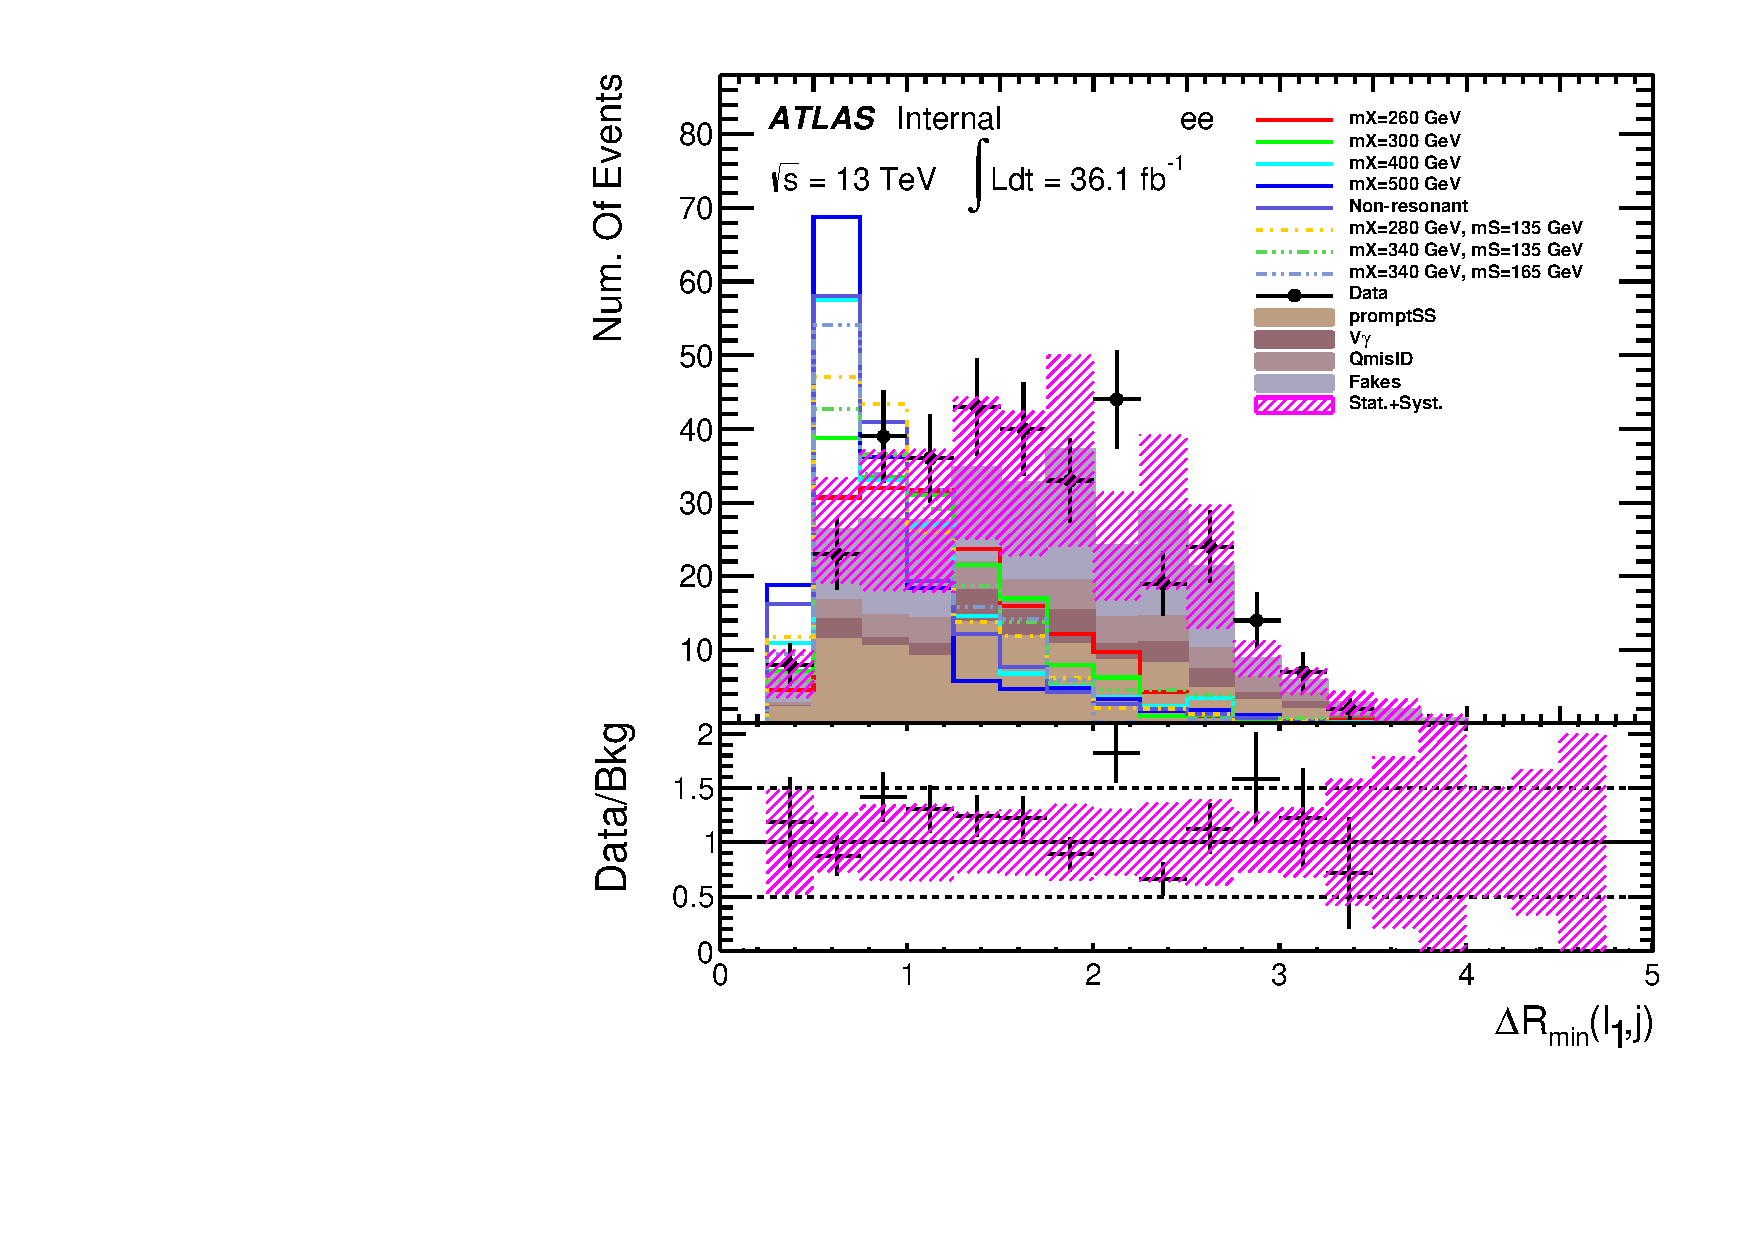
\includegraphics[width=0.9\textwidth,angle=-90]{fig/dataMC_high_Njet_CR/mindR_l1j_ee.pdf}\label{fig:dataMC_high_Njet_CR:mindRl1j_ee.pdf}
 \end{minipage}
 \begin{minipage}[t]{0.33\linewidth}
 \centering
 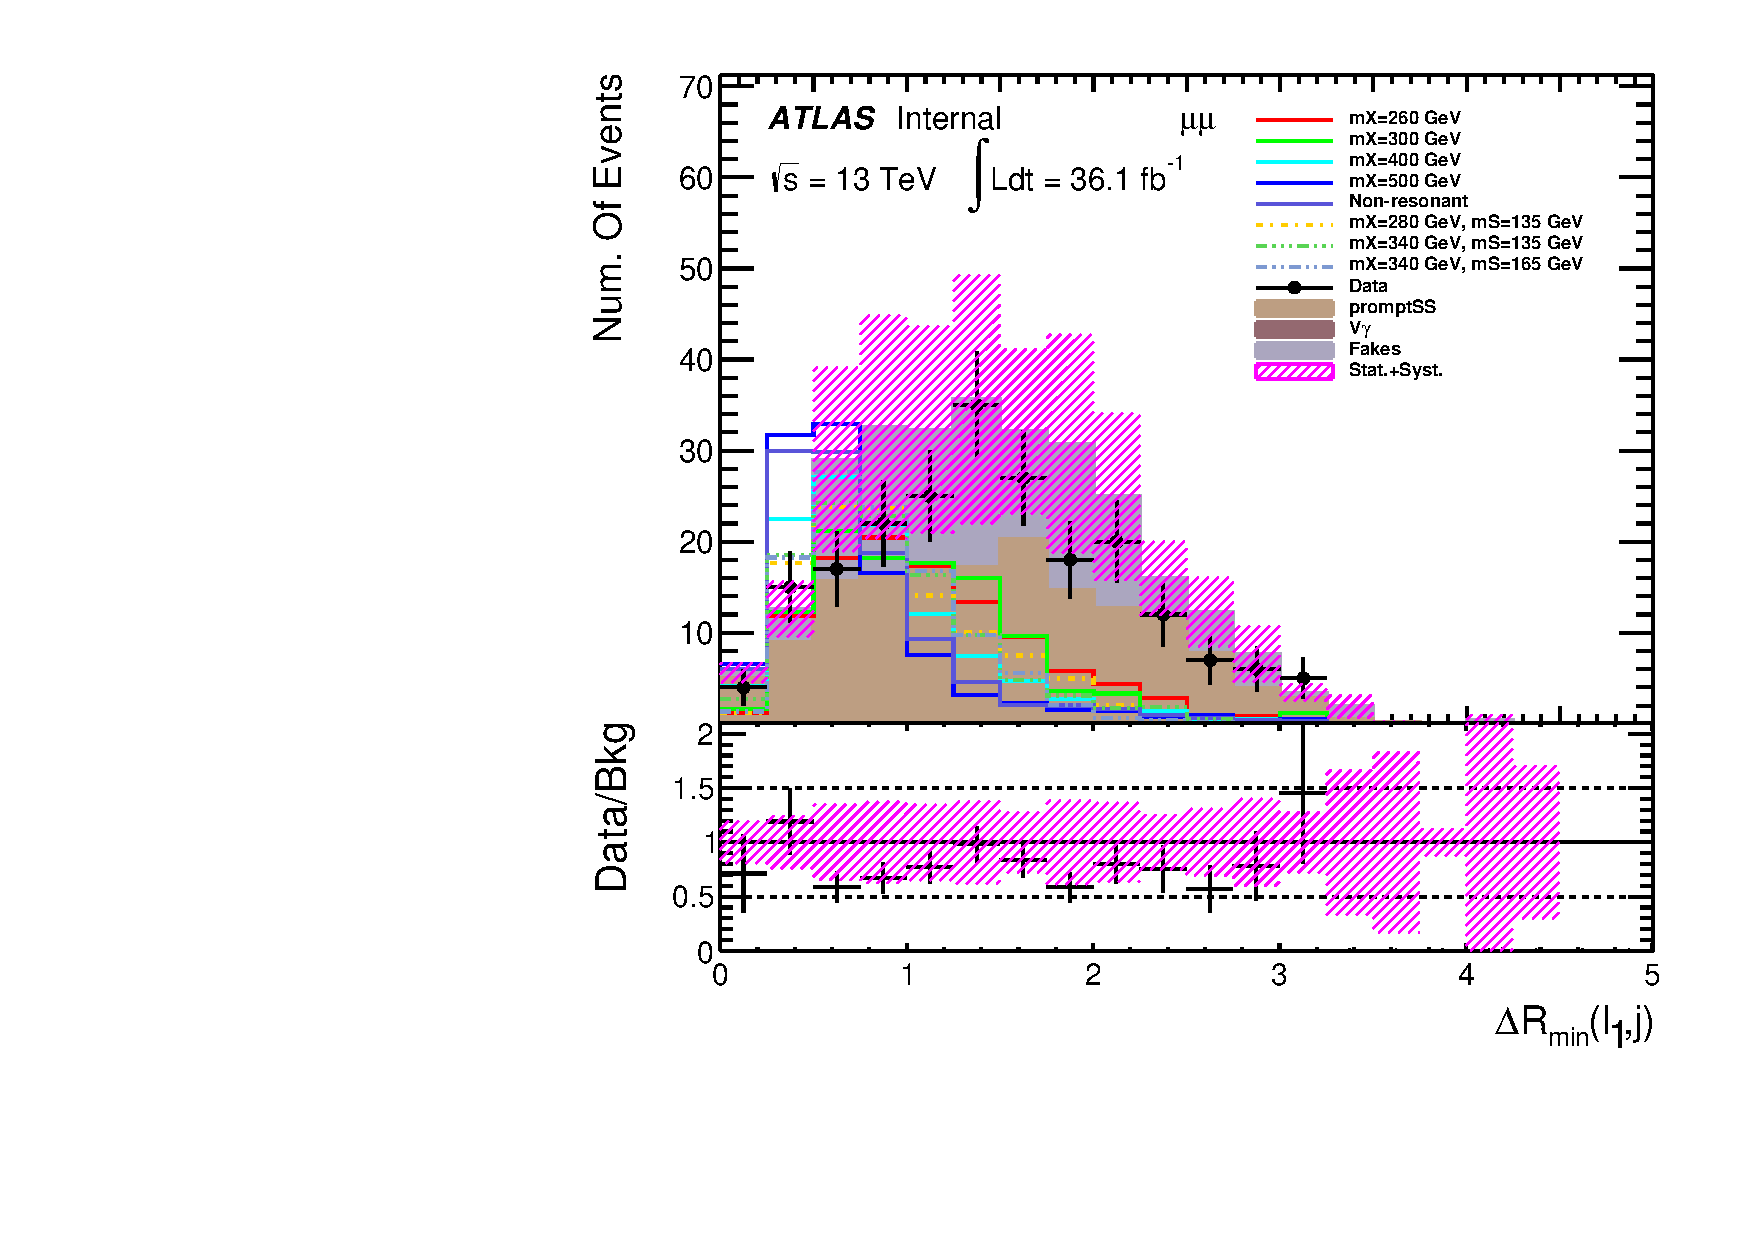
\includegraphics[width=0.9\textwidth,angle=-90]{fig/dataMC_high_Njet_CR/mindR_l1j_mumu.pdf}\label{fig:dataMC_high_Njet_CR:mindRl1j_mumu.pdf}
 \end{minipage}
  \begin{minipage}[t]{0.33\linewidth}
 \centering
 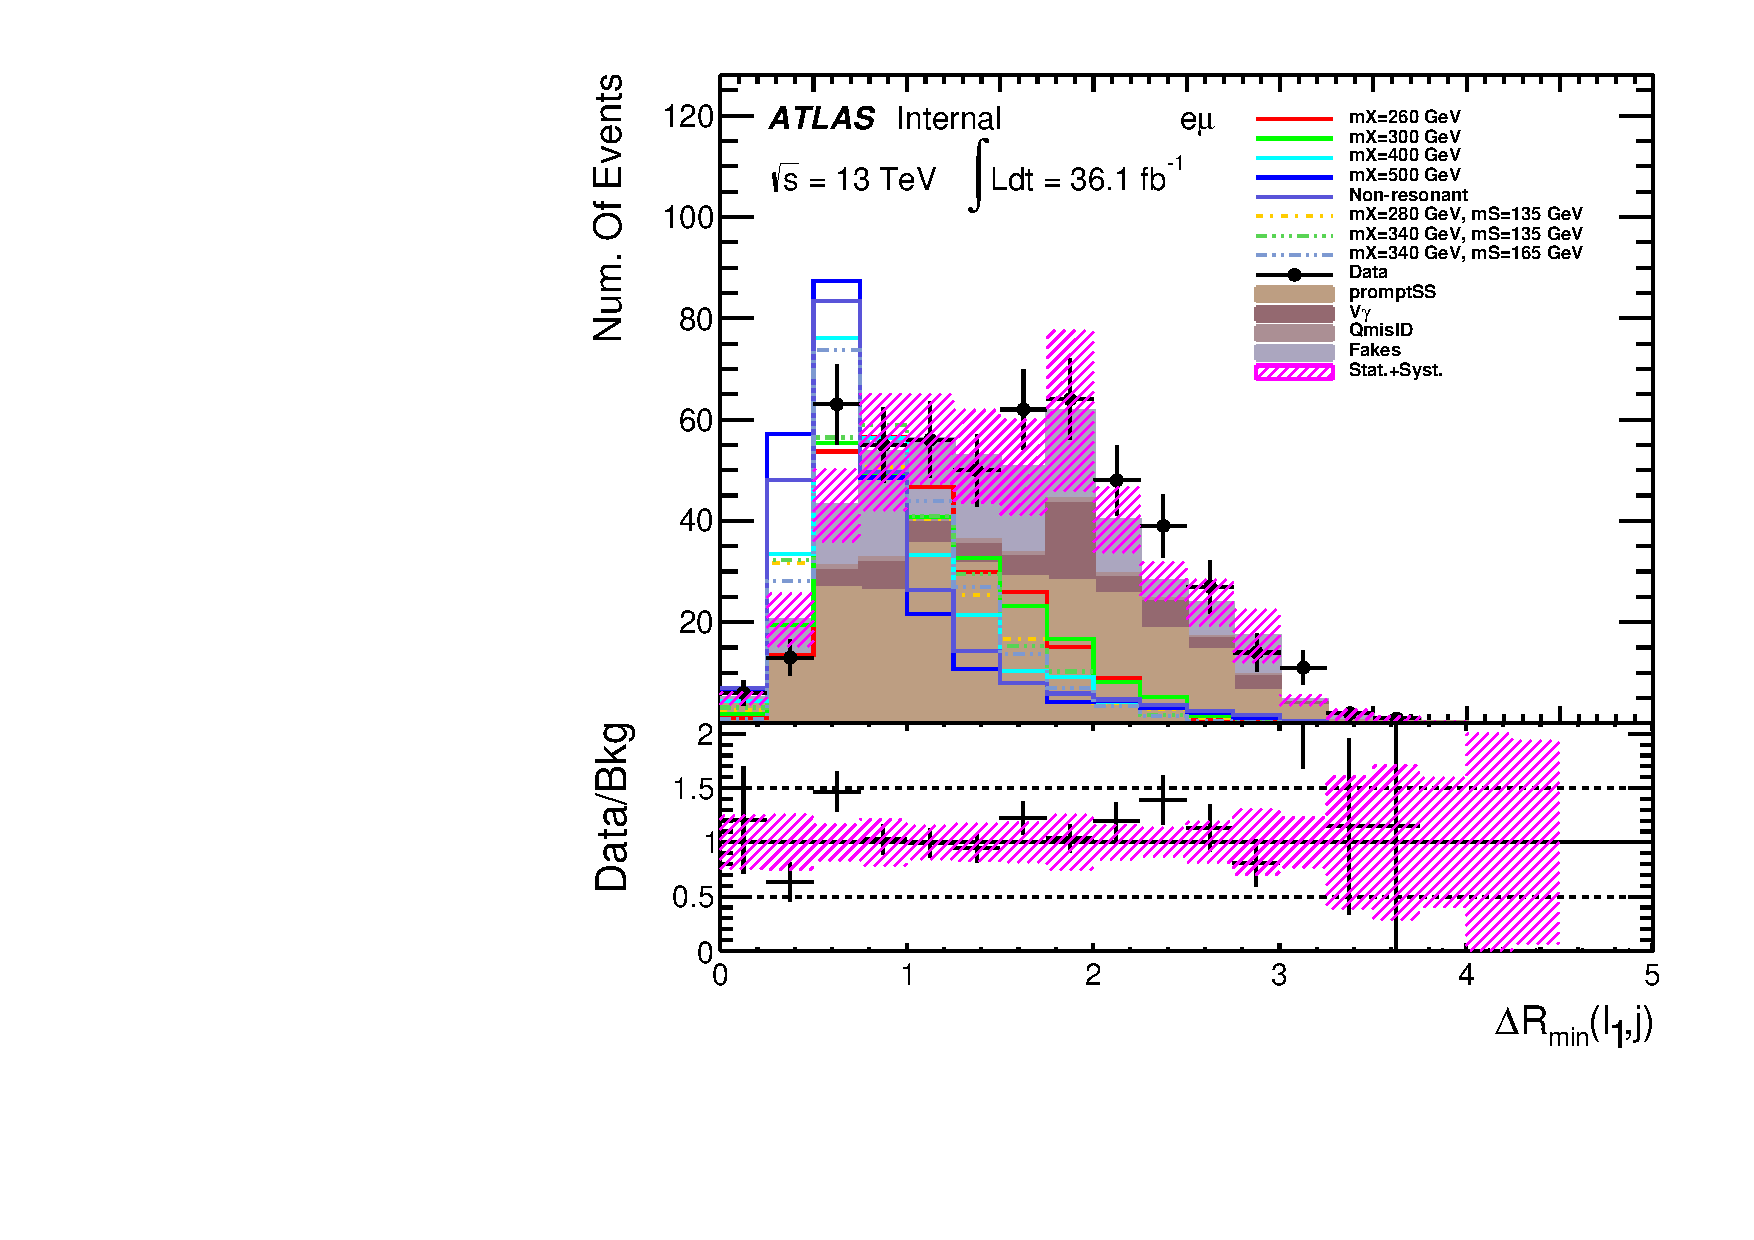
\includegraphics[width=0.9\textwidth,angle=-90]{fig/dataMC_high_Njet_CR/mindR_l1j_emu.pdf}\label{fig:dataMC_high_Njet_CR:mindRl1j_emu.pdf}
 \end{minipage}
\begin{minipage}[t]{0.33\linewidth}
 \centering
 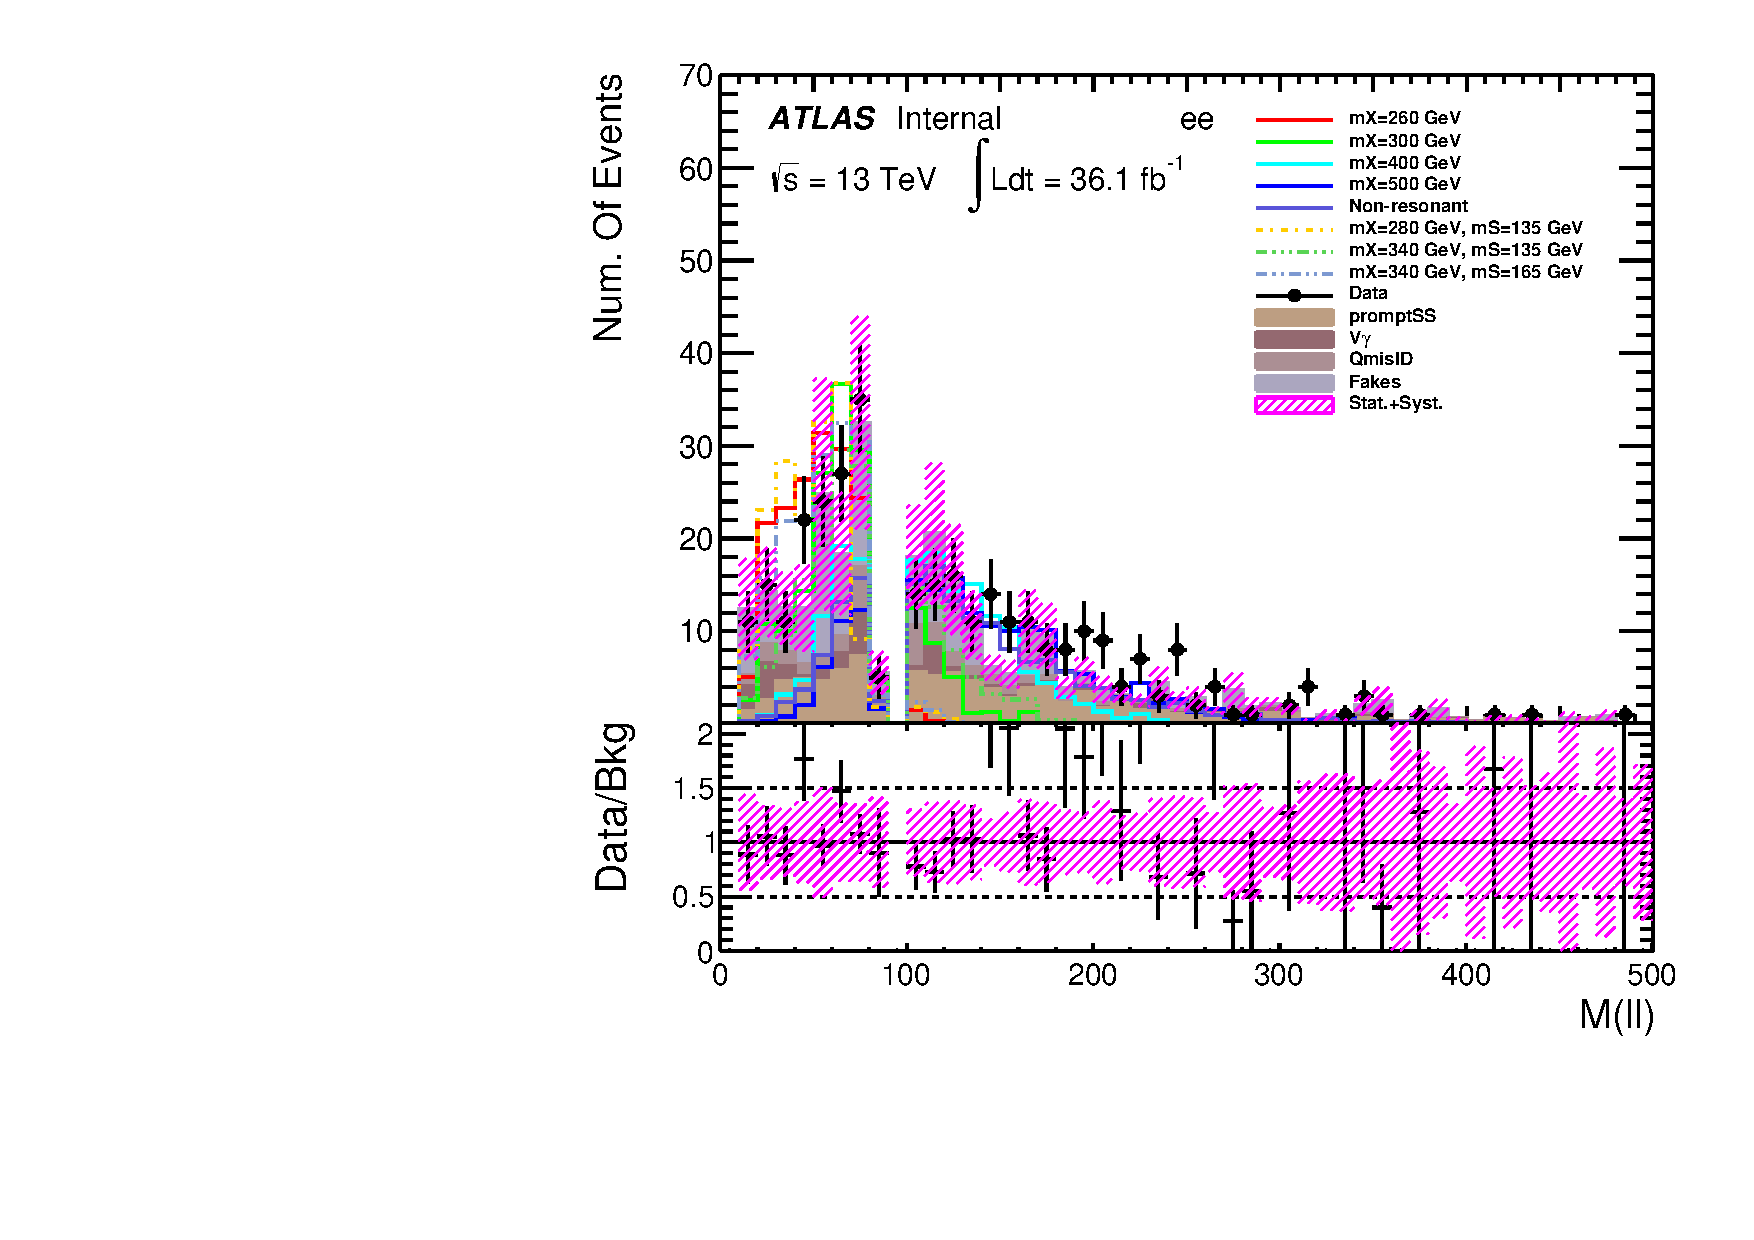
\includegraphics[width=0.9\textwidth,angle=-90]{fig/dataMC_high_Njet_CR/m_ll_ee.pdf}
 \label{fig:dataMC_high_Njet_CR:m_ll_ee.pdf}
 \end{minipage}
 \begin{minipage}[t]{0.33\linewidth}
 \centering
 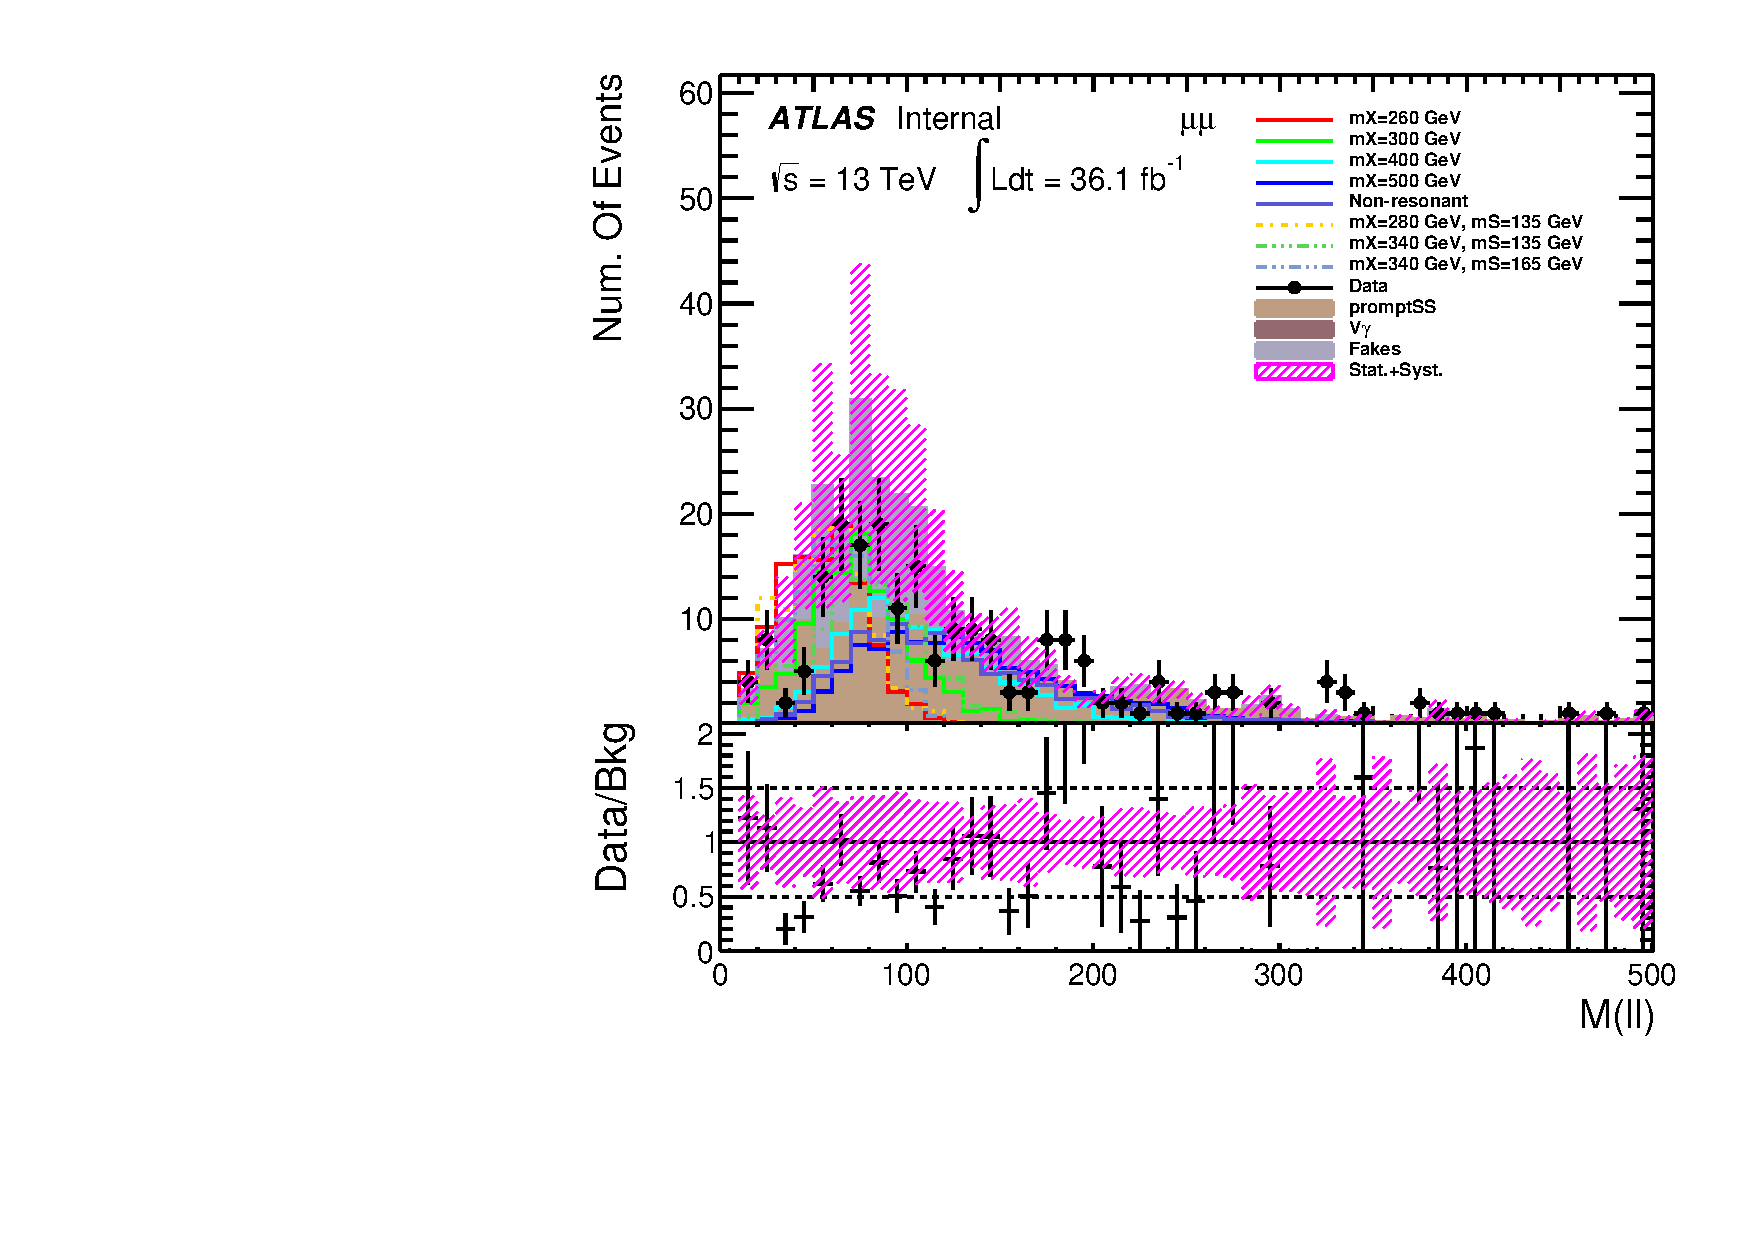
\includegraphics[width=0.9\textwidth,angle=-90]{fig/dataMC_high_Njet_CR/m_ll_mumu.pdf}
 \label{fig:dataMC_high_Njet_CR:m_ll_mumu.pdf}
 \end{minipage}
 \begin{minipage}[t]{0.33\linewidth}
 \centering
 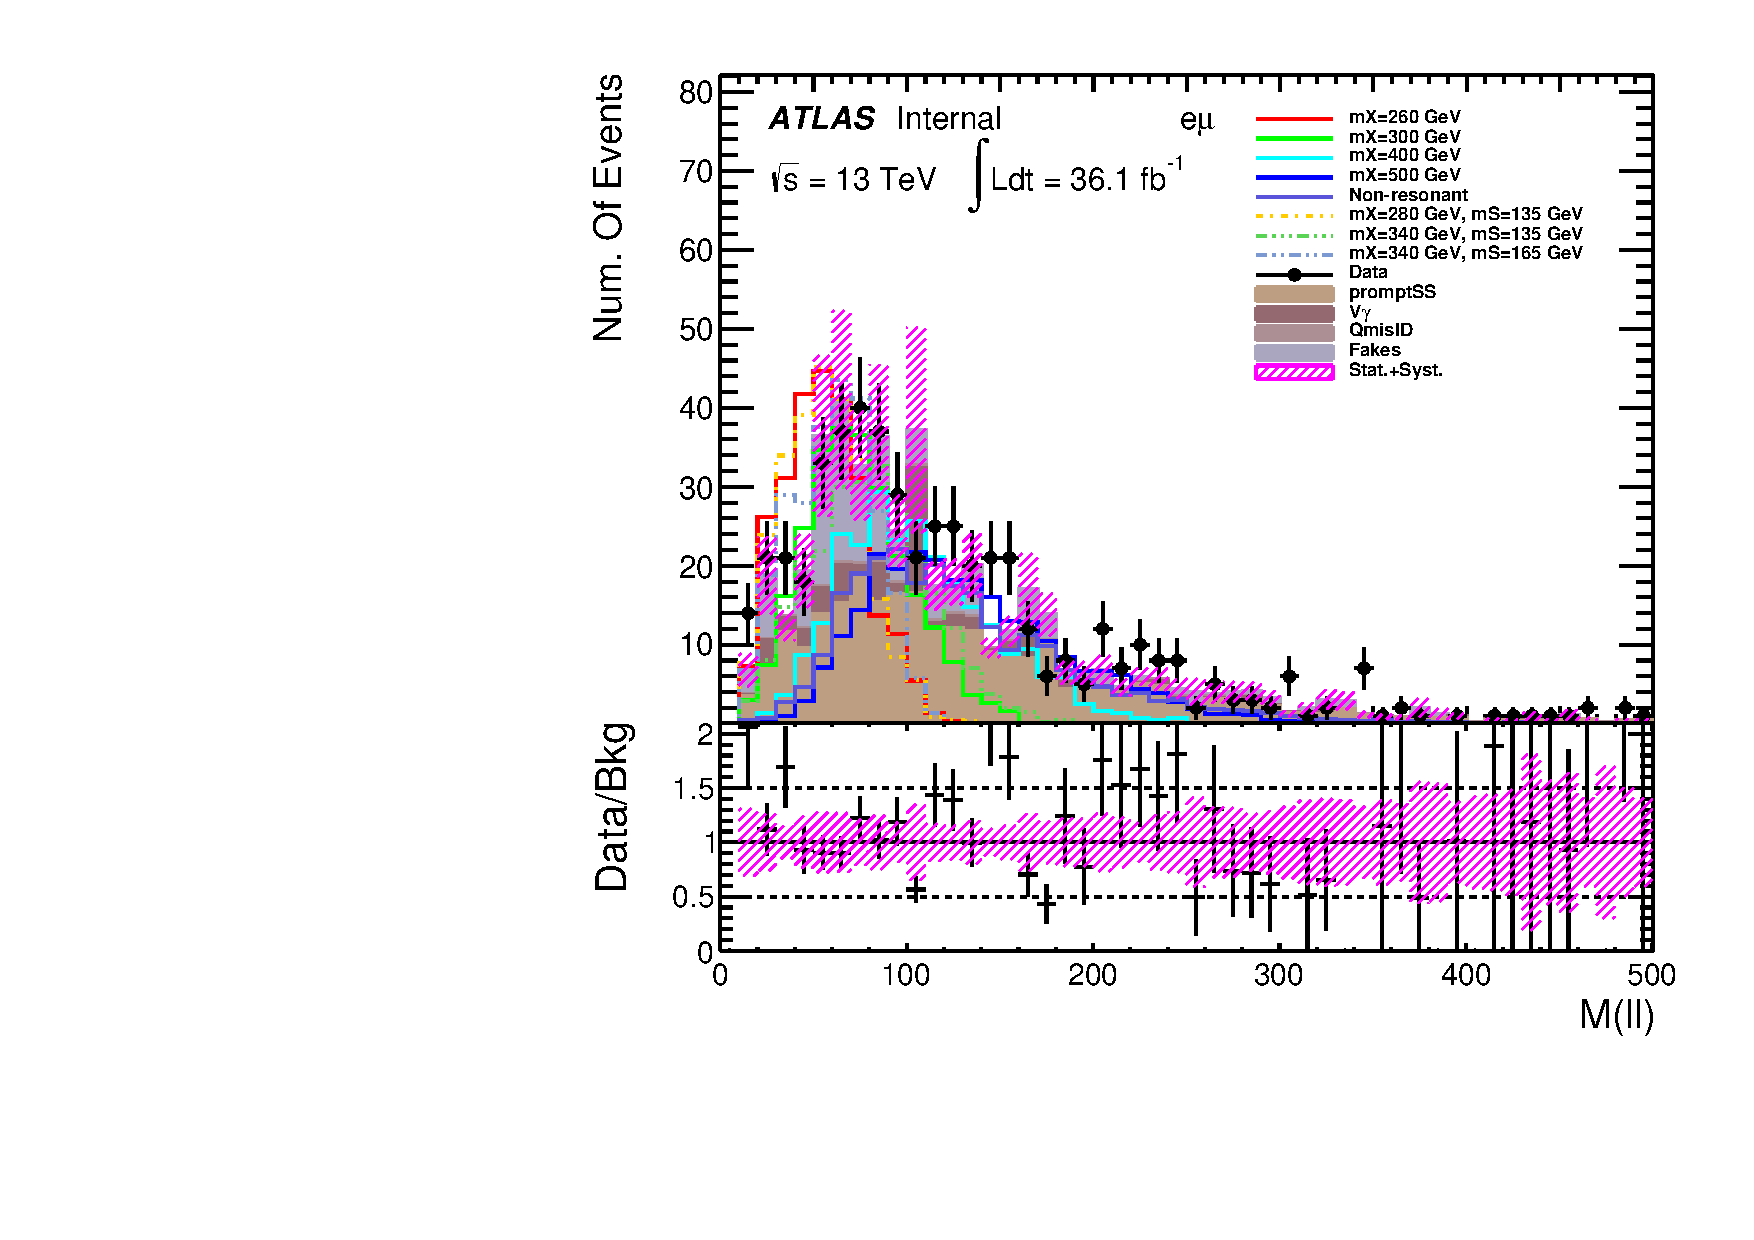
\includegraphics[width=0.9\textwidth,angle=-90]{fig/dataMC_high_Njet_CR/m_ll_emu.pdf}
 \label{fig:dataMC_high_Njet_CR:m_ll_emu.pdf}
 \end{minipage}
\begin{minipage}[t]{0.33\linewidth}
 \centering
 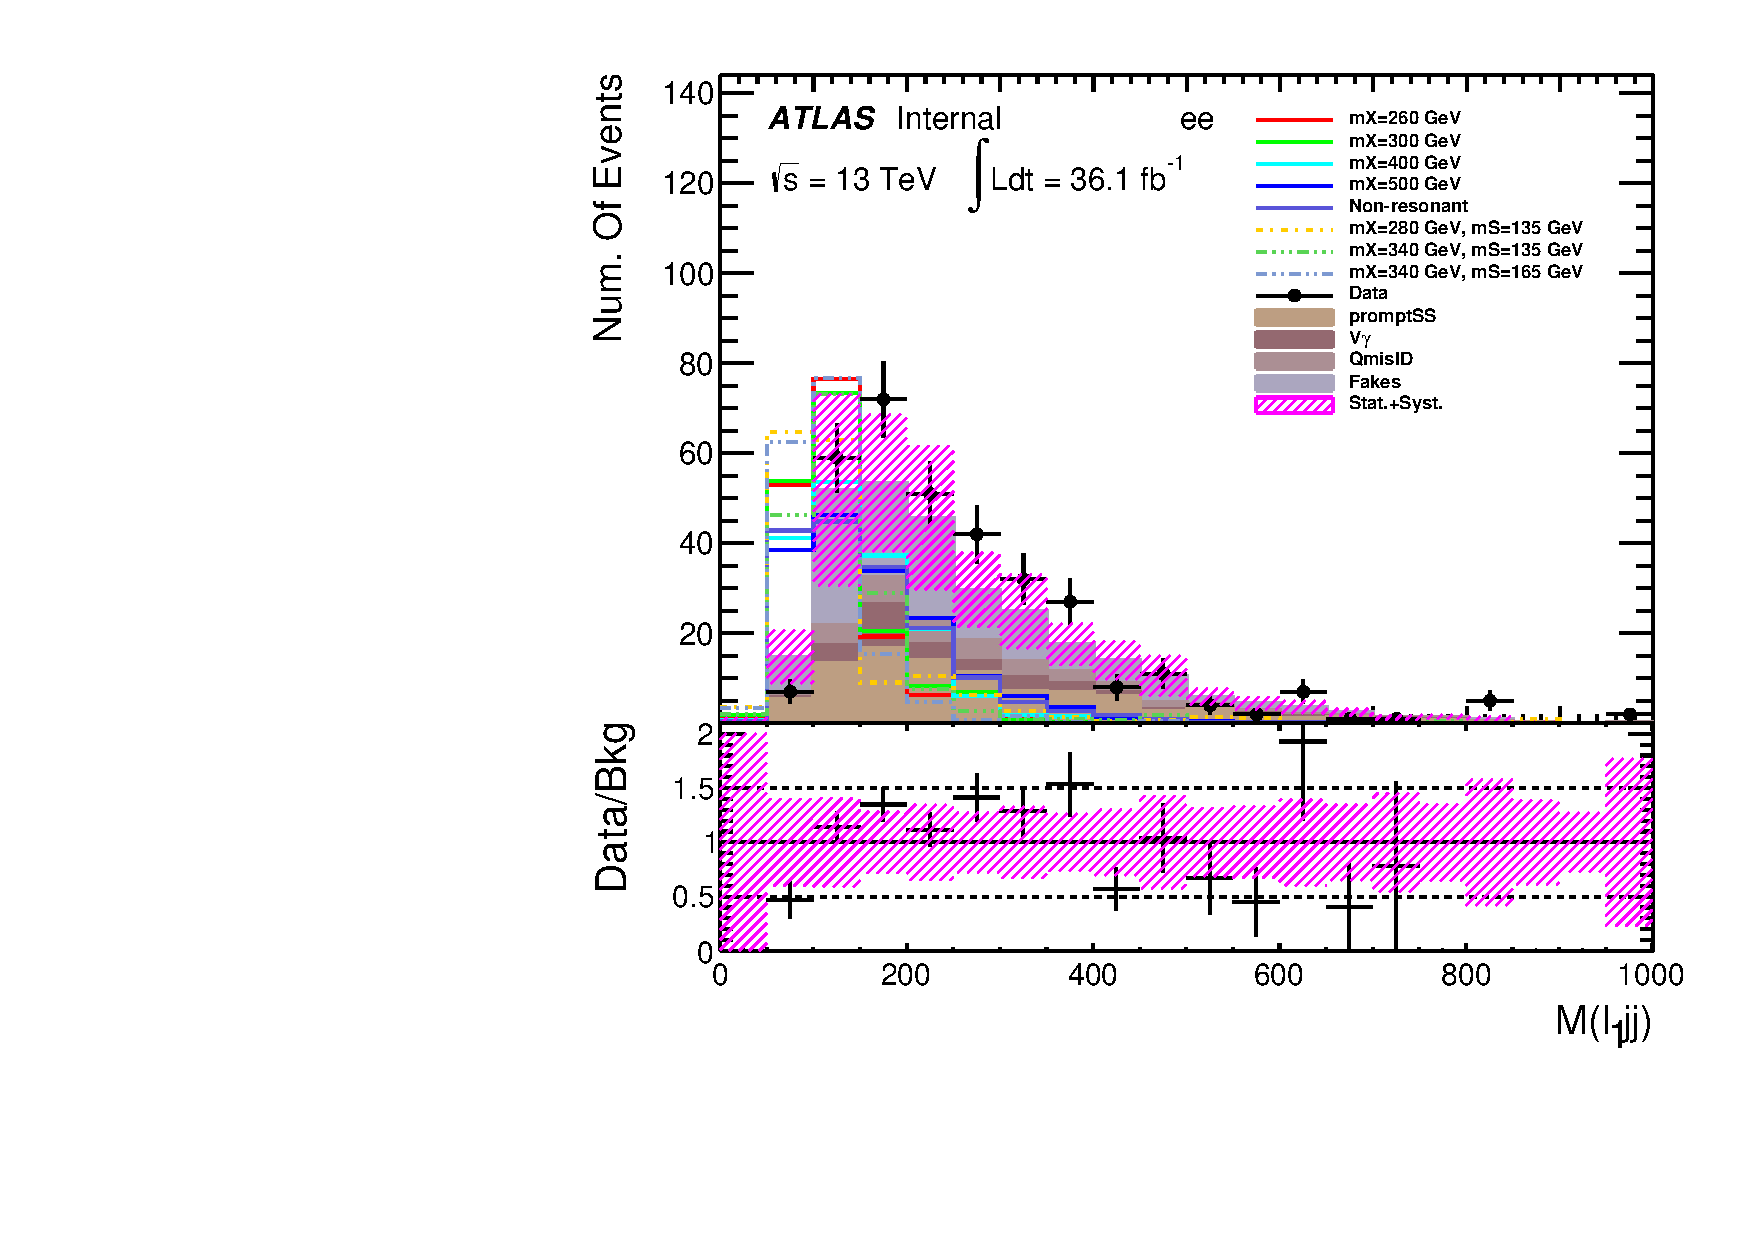
\includegraphics[width=0.9\textwidth,angle=-90]{fig/dataMC_high_Njet_CR/m_l1jj_ee.pdf}\label{fig:dataMC_high_Njet_CR:m_l1jj_ee.pdf}
 \end{minipage}
  \begin{minipage}[t]{0.33\linewidth}
 \centering
 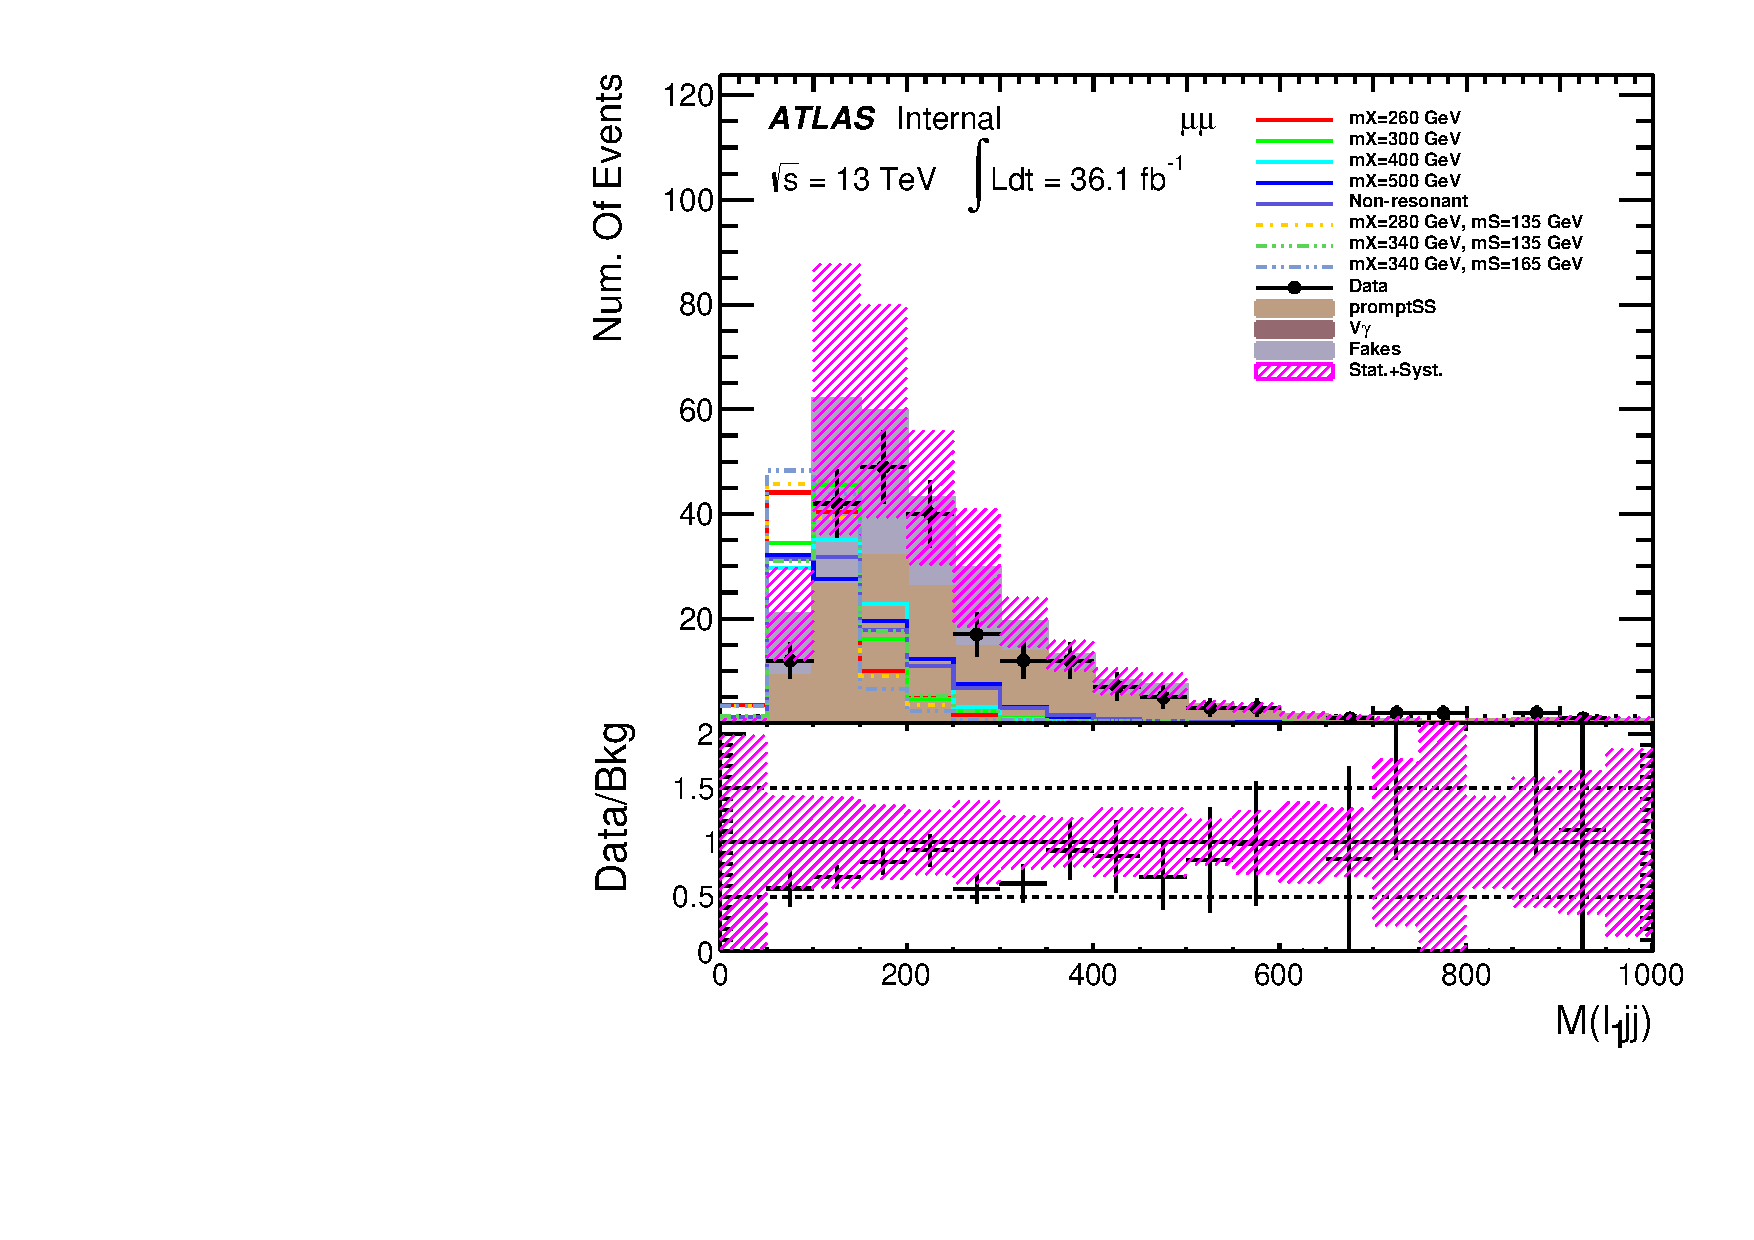
\includegraphics[width=0.9\textwidth,angle=-90]{fig/dataMC_high_Njet_CR/m_l1jj_mumu.pdf}\label{fig:dataMC_high_Njet_CR:m_l1jj_mumu.pdf}
 \end{minipage}
 \begin{minipage}[t]{0.33\linewidth}
 \centering
 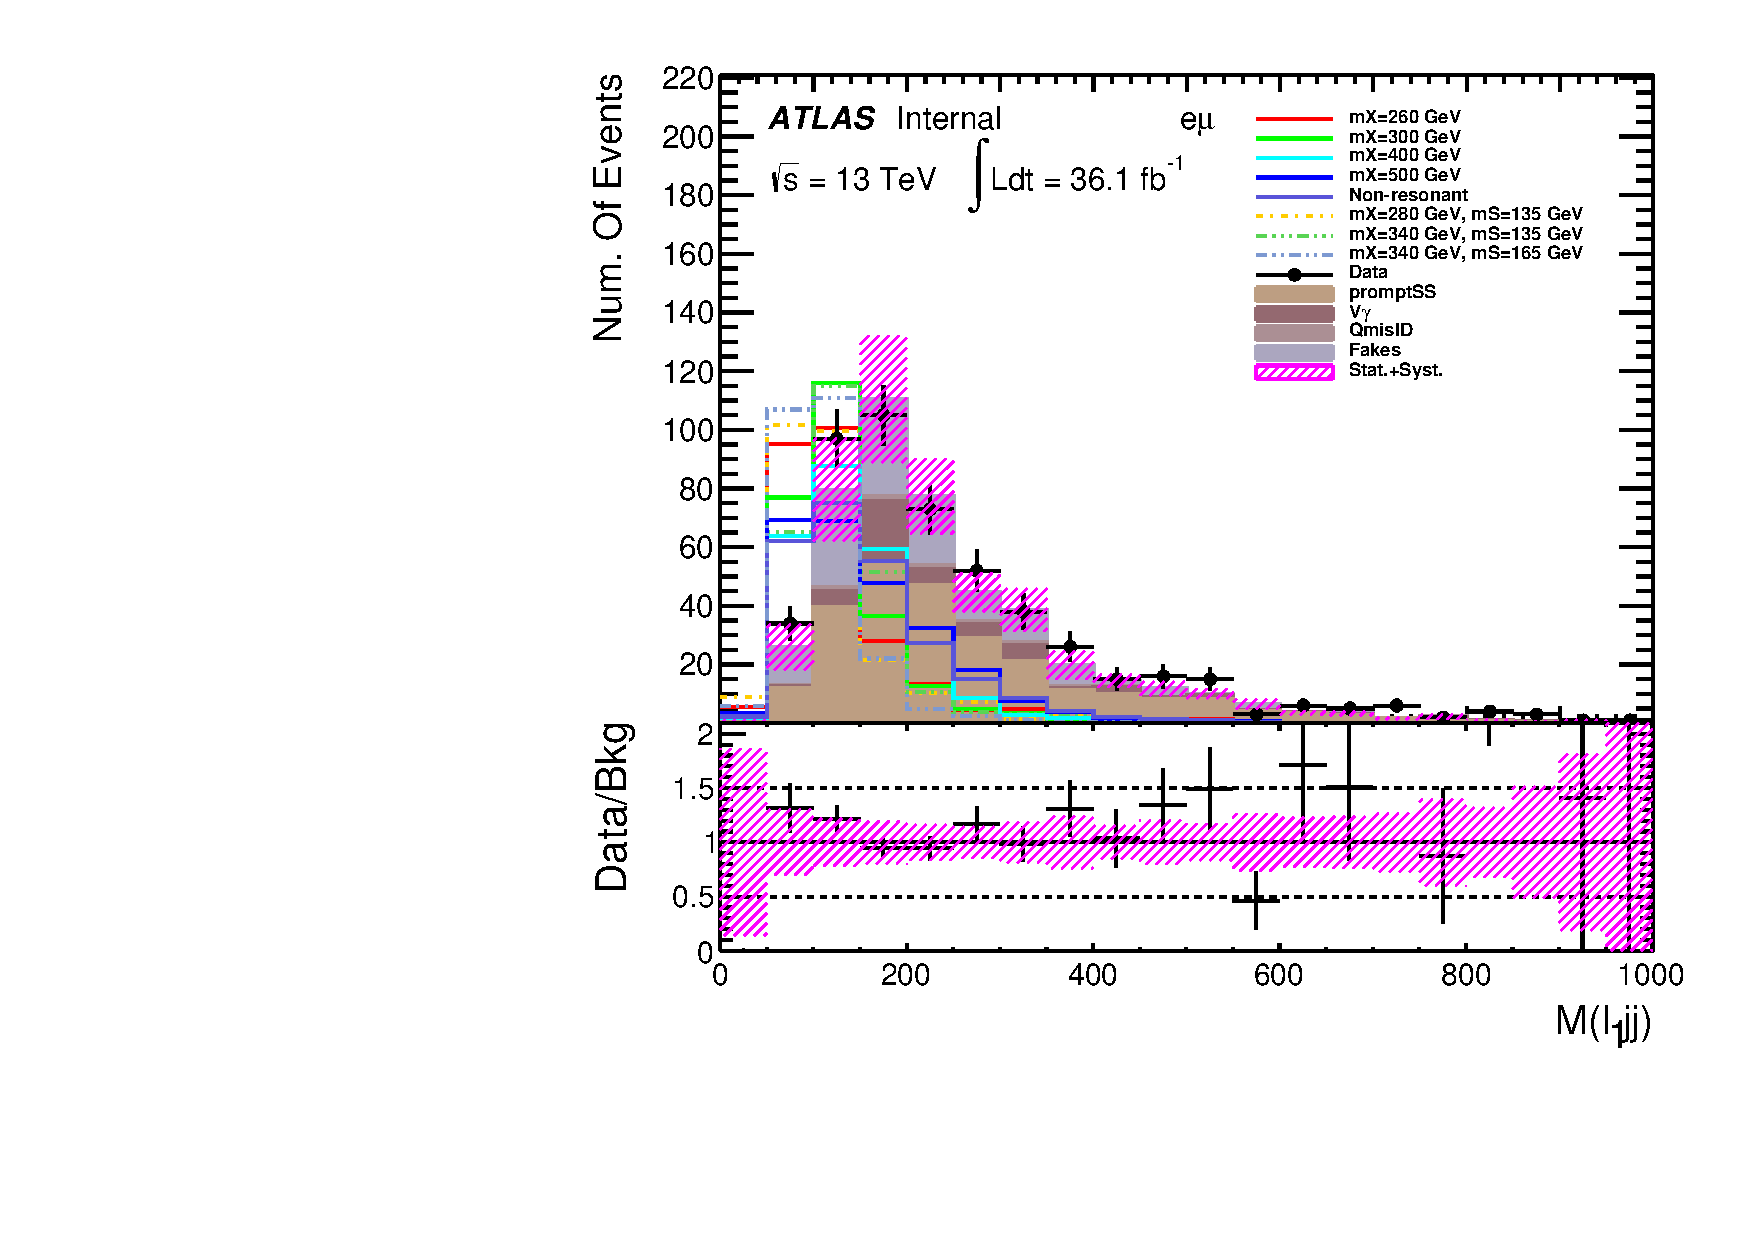
\includegraphics[width=0.9\textwidth,angle=-90]{fig/dataMC_high_Njet_CR/m_l1jj_emu.pdf}\label{fig:dataMC_high_Njet_CR:m_l1jj_emu.pdf}
 \end{minipage}
 \caption{用于低质量信号优化的运动学变量分布,对应$N_{\text{jet}}\geq3$。}
 %\caption{The distributions of kinematic variables that are used to form optimization selections at pre-selection level, corresponding to $N_{\text{jet}}\geq3$. Left: $ee$, middle: $\mu\mu$, right: $e\mu$. PromptSS and $V+\gamma$ are normalized to the luminosity of 36.1 fb$^{-1}$.}
\label{fig:SigOpt_high_kine}
\end{figure}
\begin{figure}[h]
\begin{center}
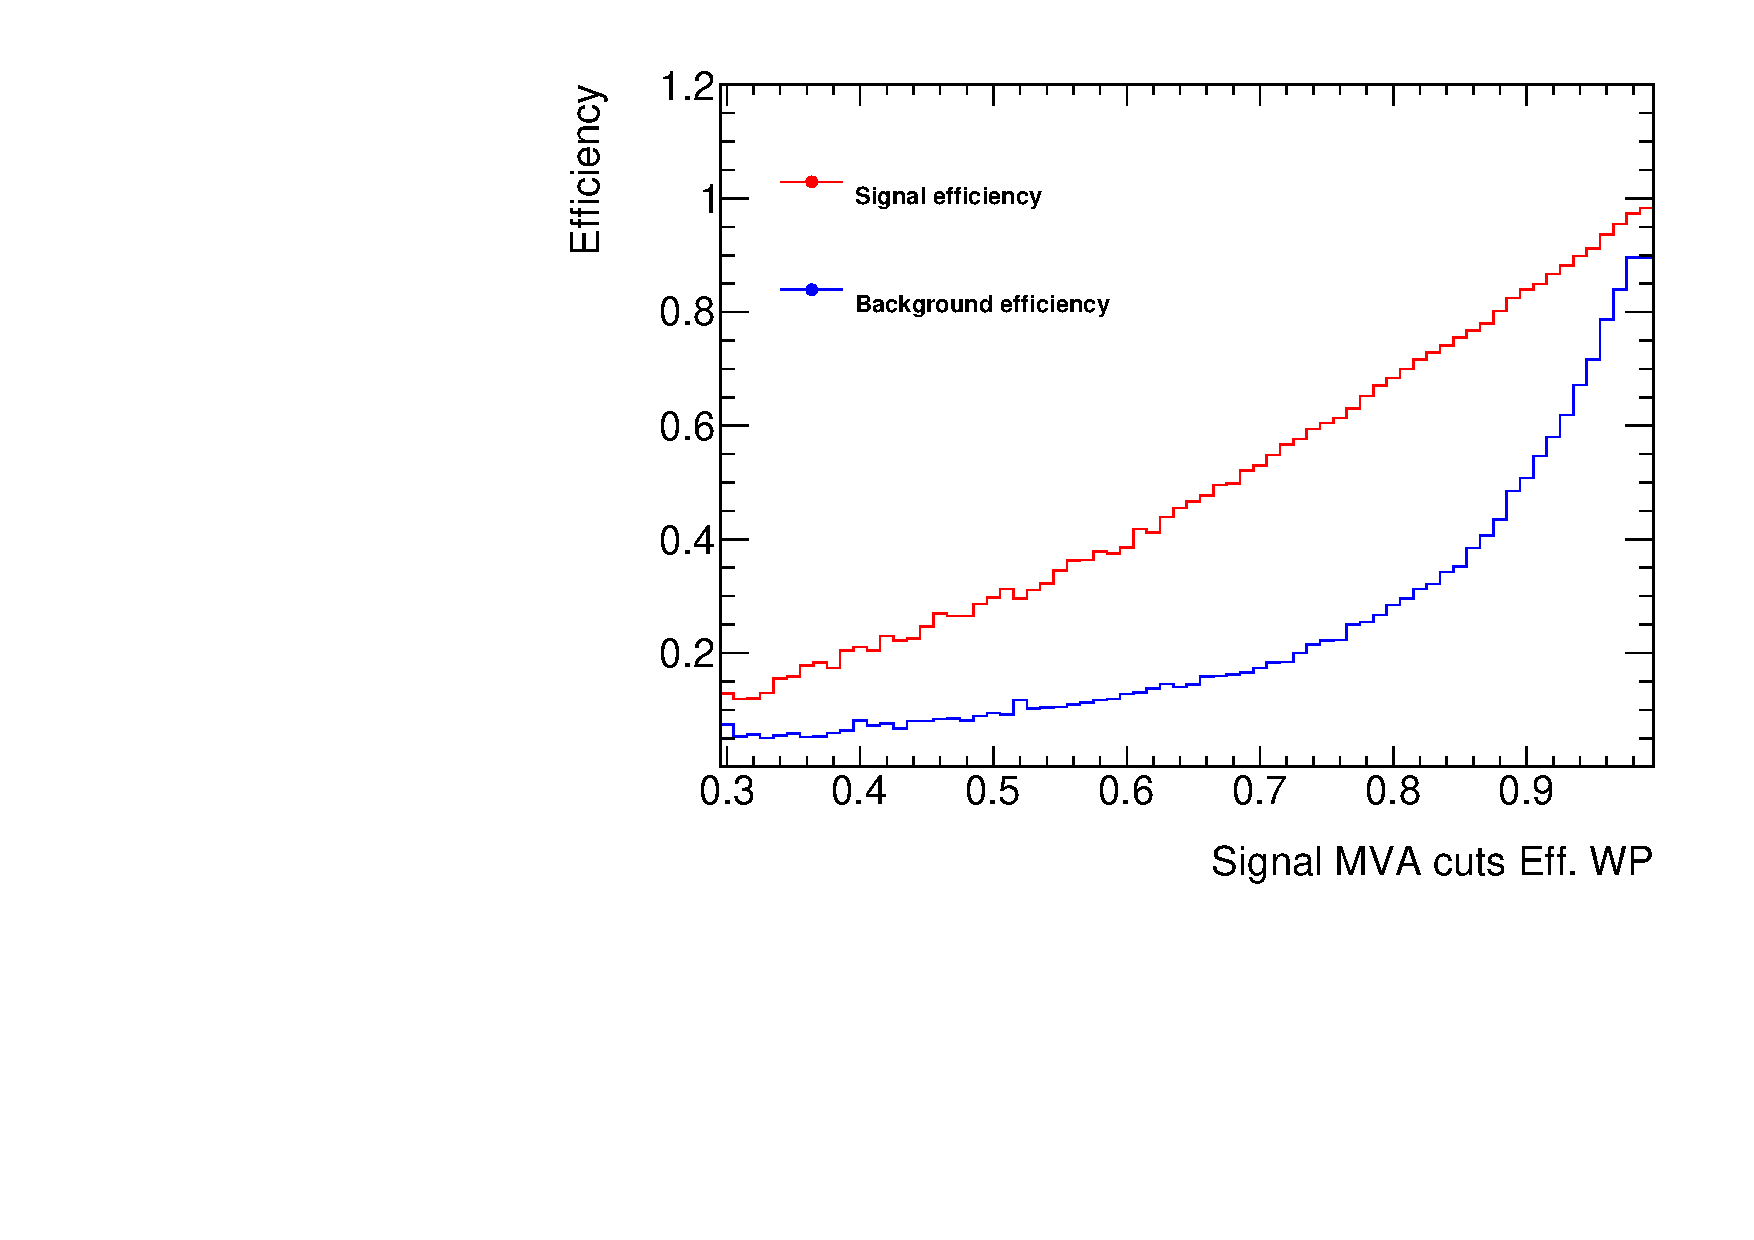
\includegraphics[width = 0.3\textwidth,angle=-90]{fig/SigOpt/nonres/Efficiency_mumu.pdf}
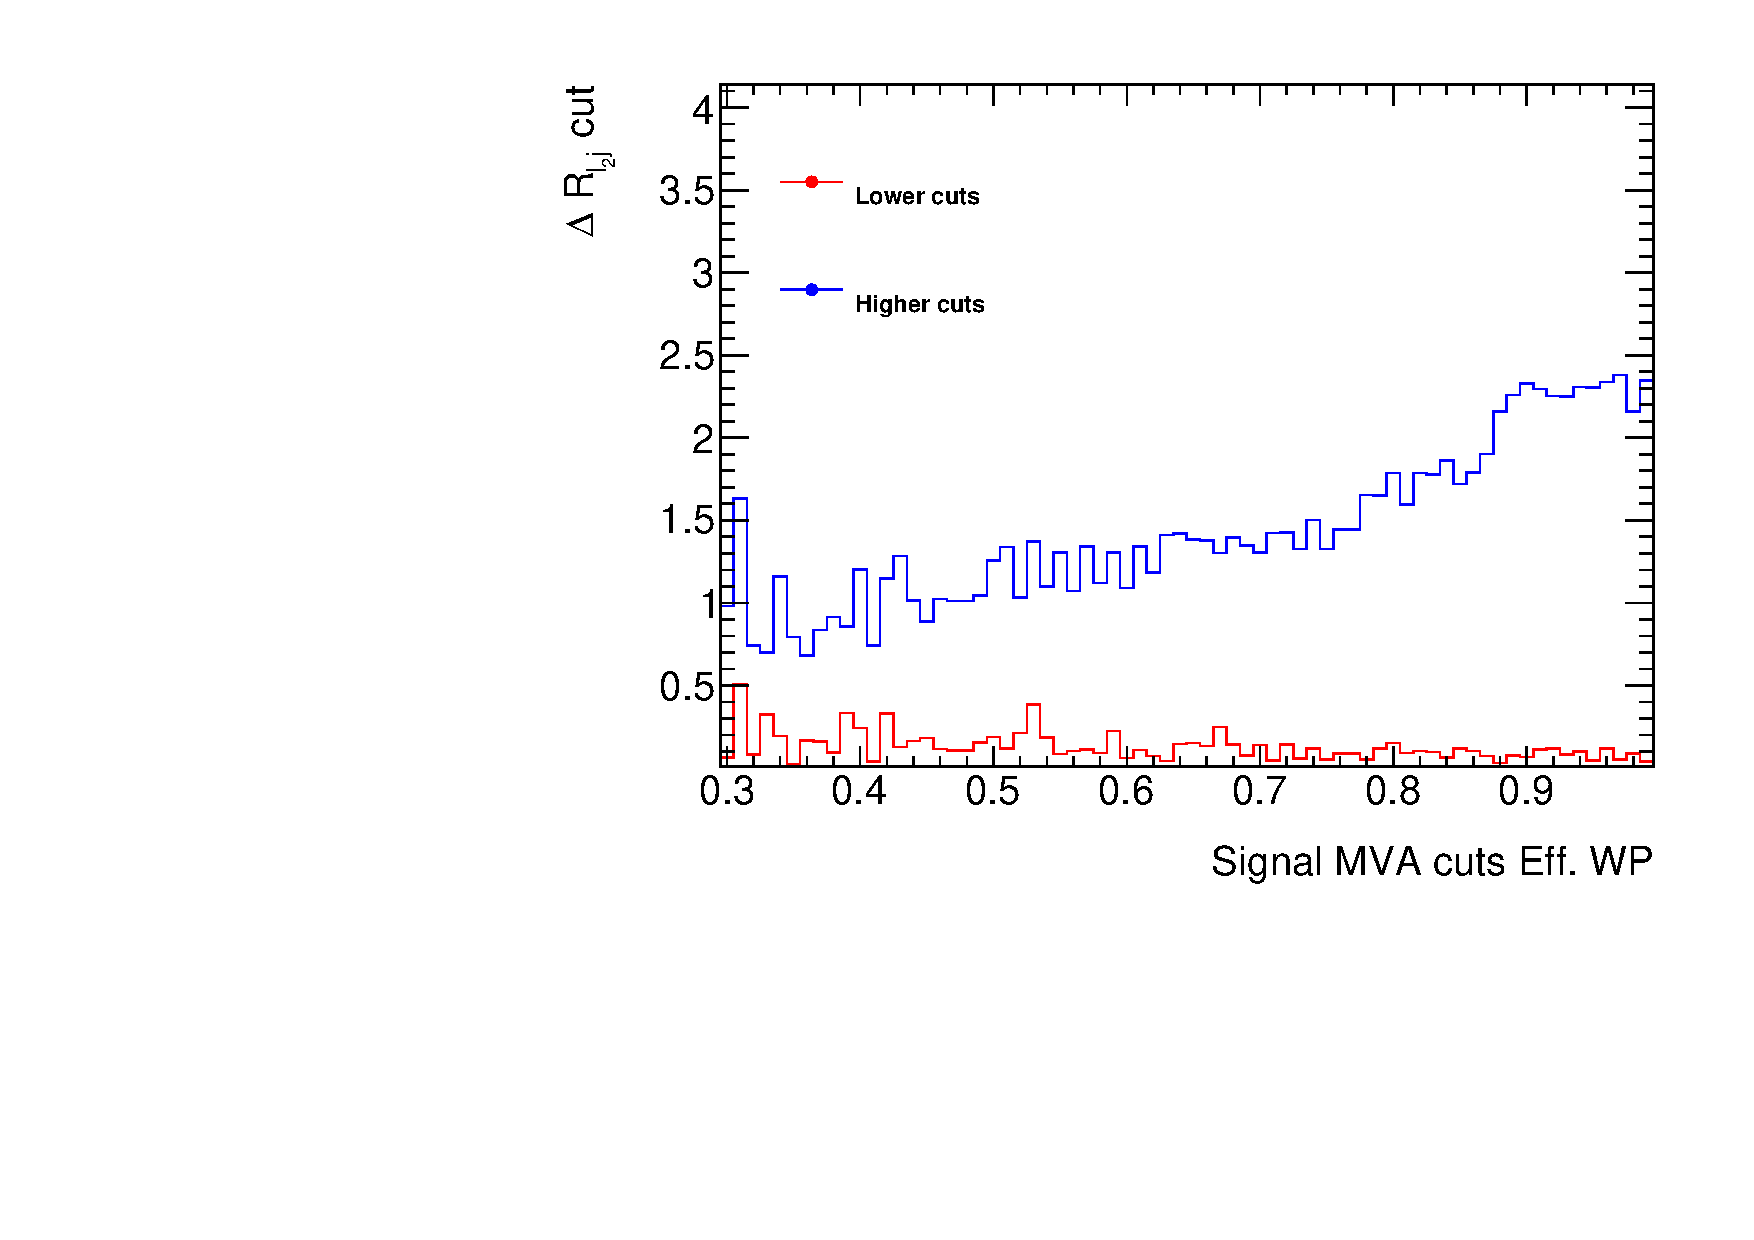
\includegraphics[width = 0.3\textwidth,angle=-90]{fig/SigOpt/nonres/mindR_l2j_mumu.pdf}
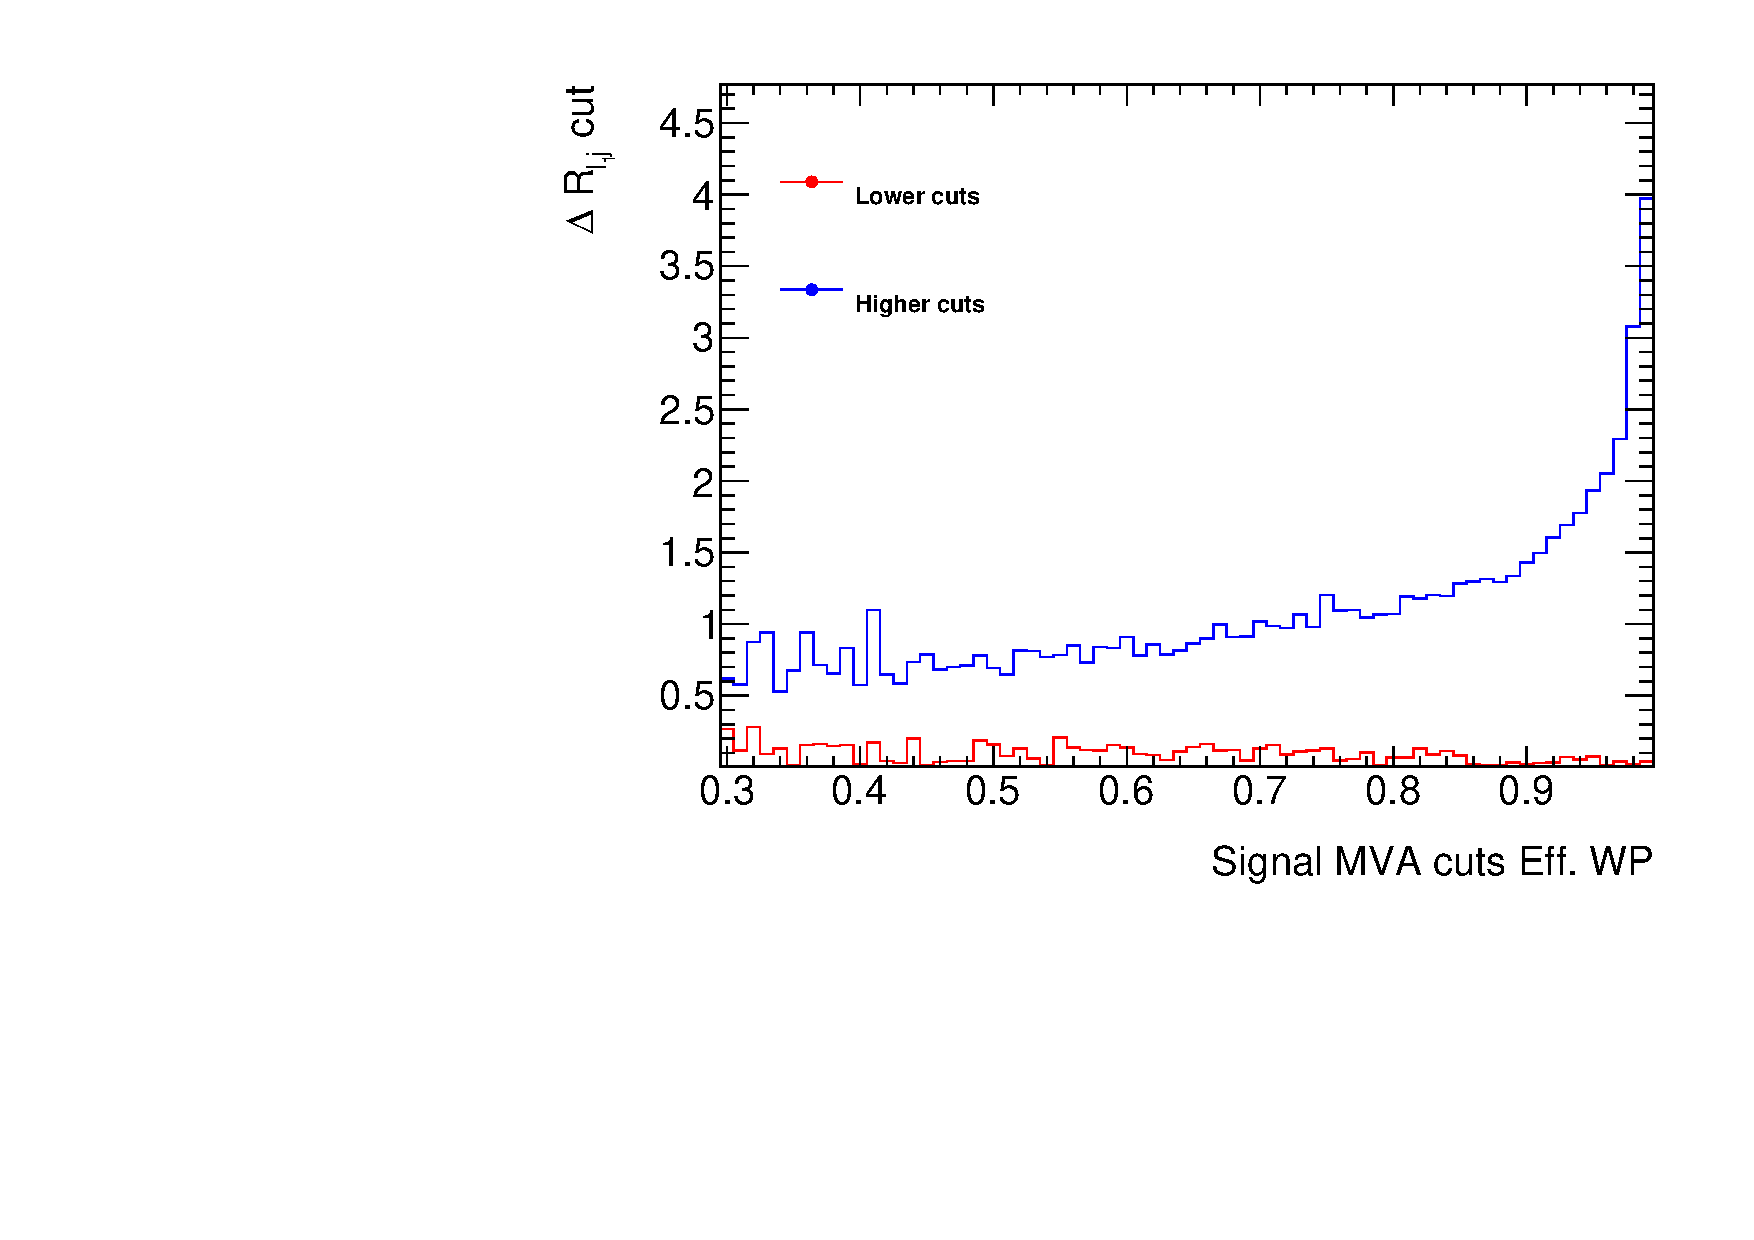
\includegraphics[width = 0.3\textwidth,angle=-90]{fig/SigOpt/nonres/mindR_l1j_mumu.pdf}
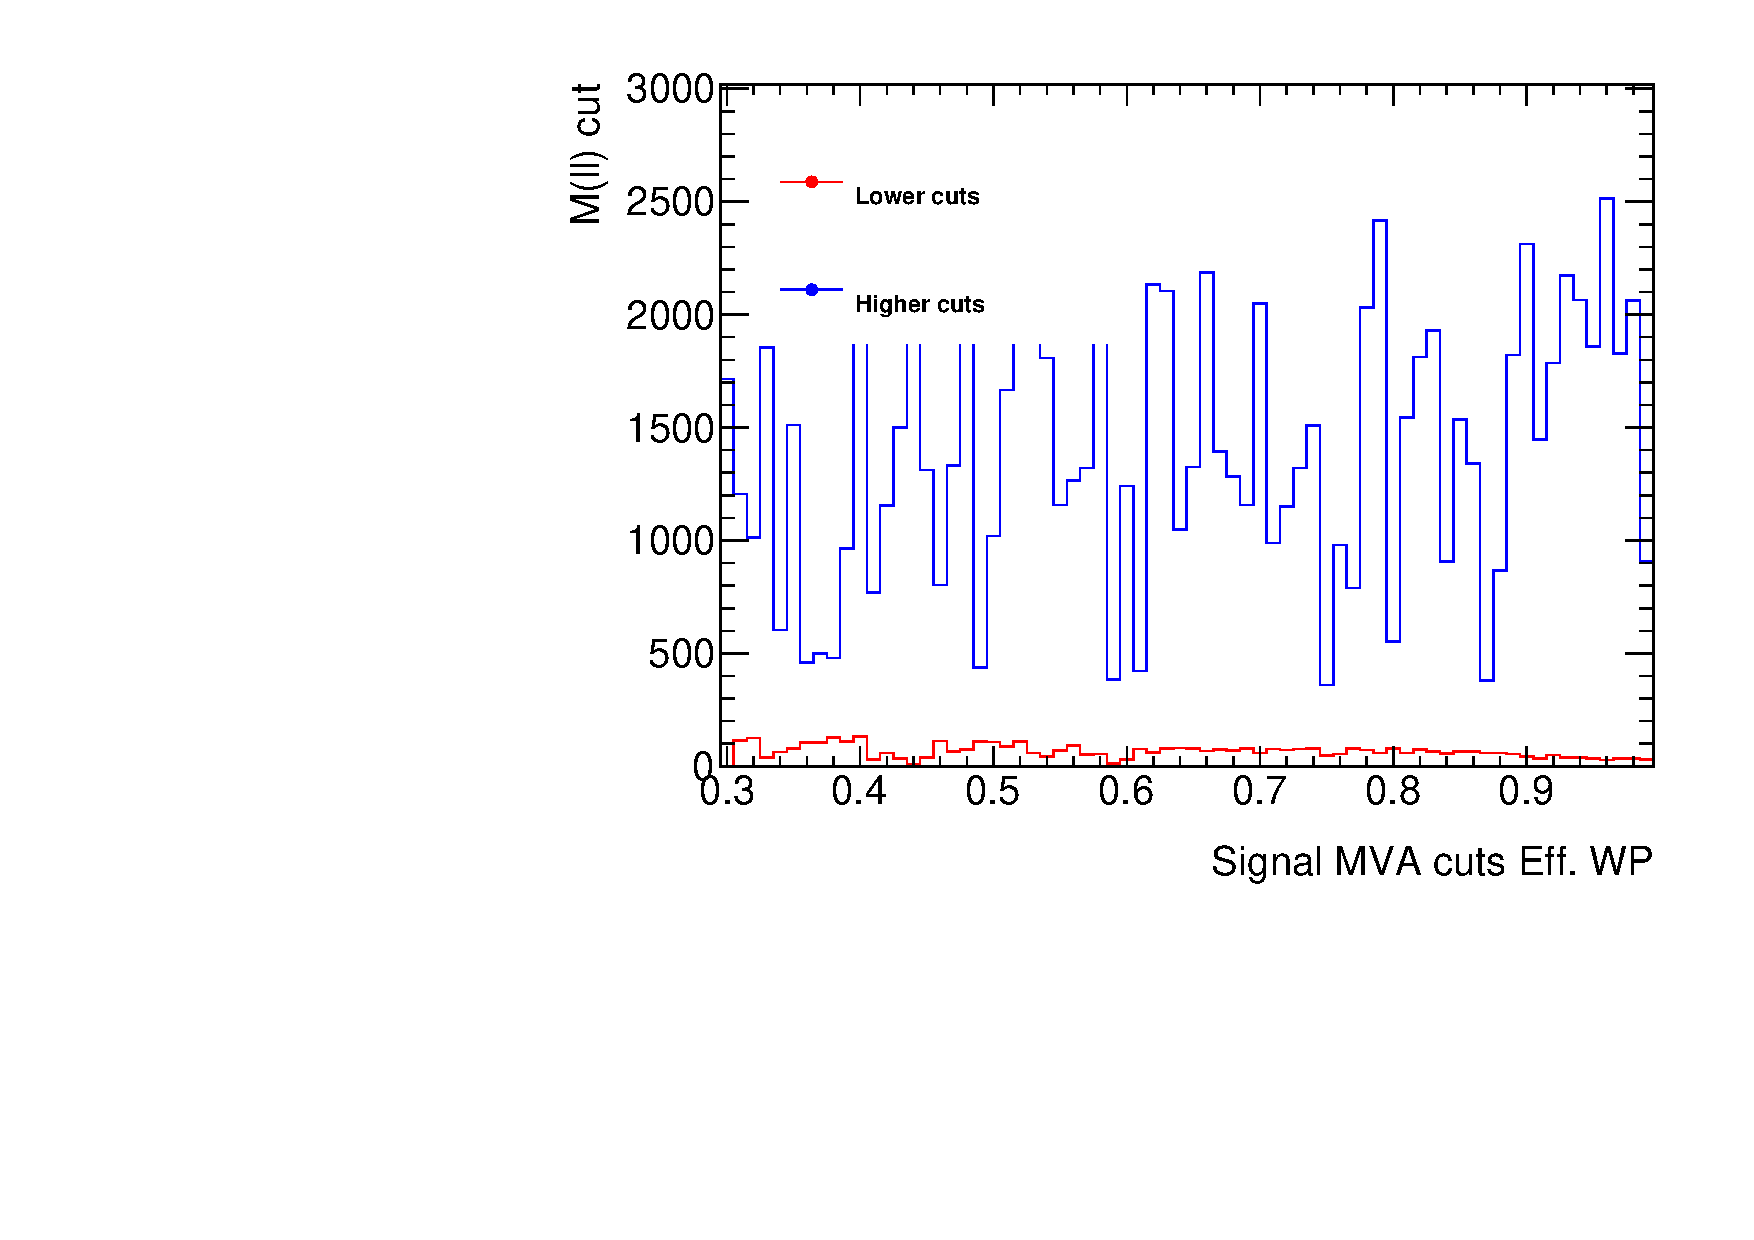
\includegraphics[width = 0.3\textwidth,angle=-90]{fig/SigOpt/nonres/m_ll_mumu.pdf}
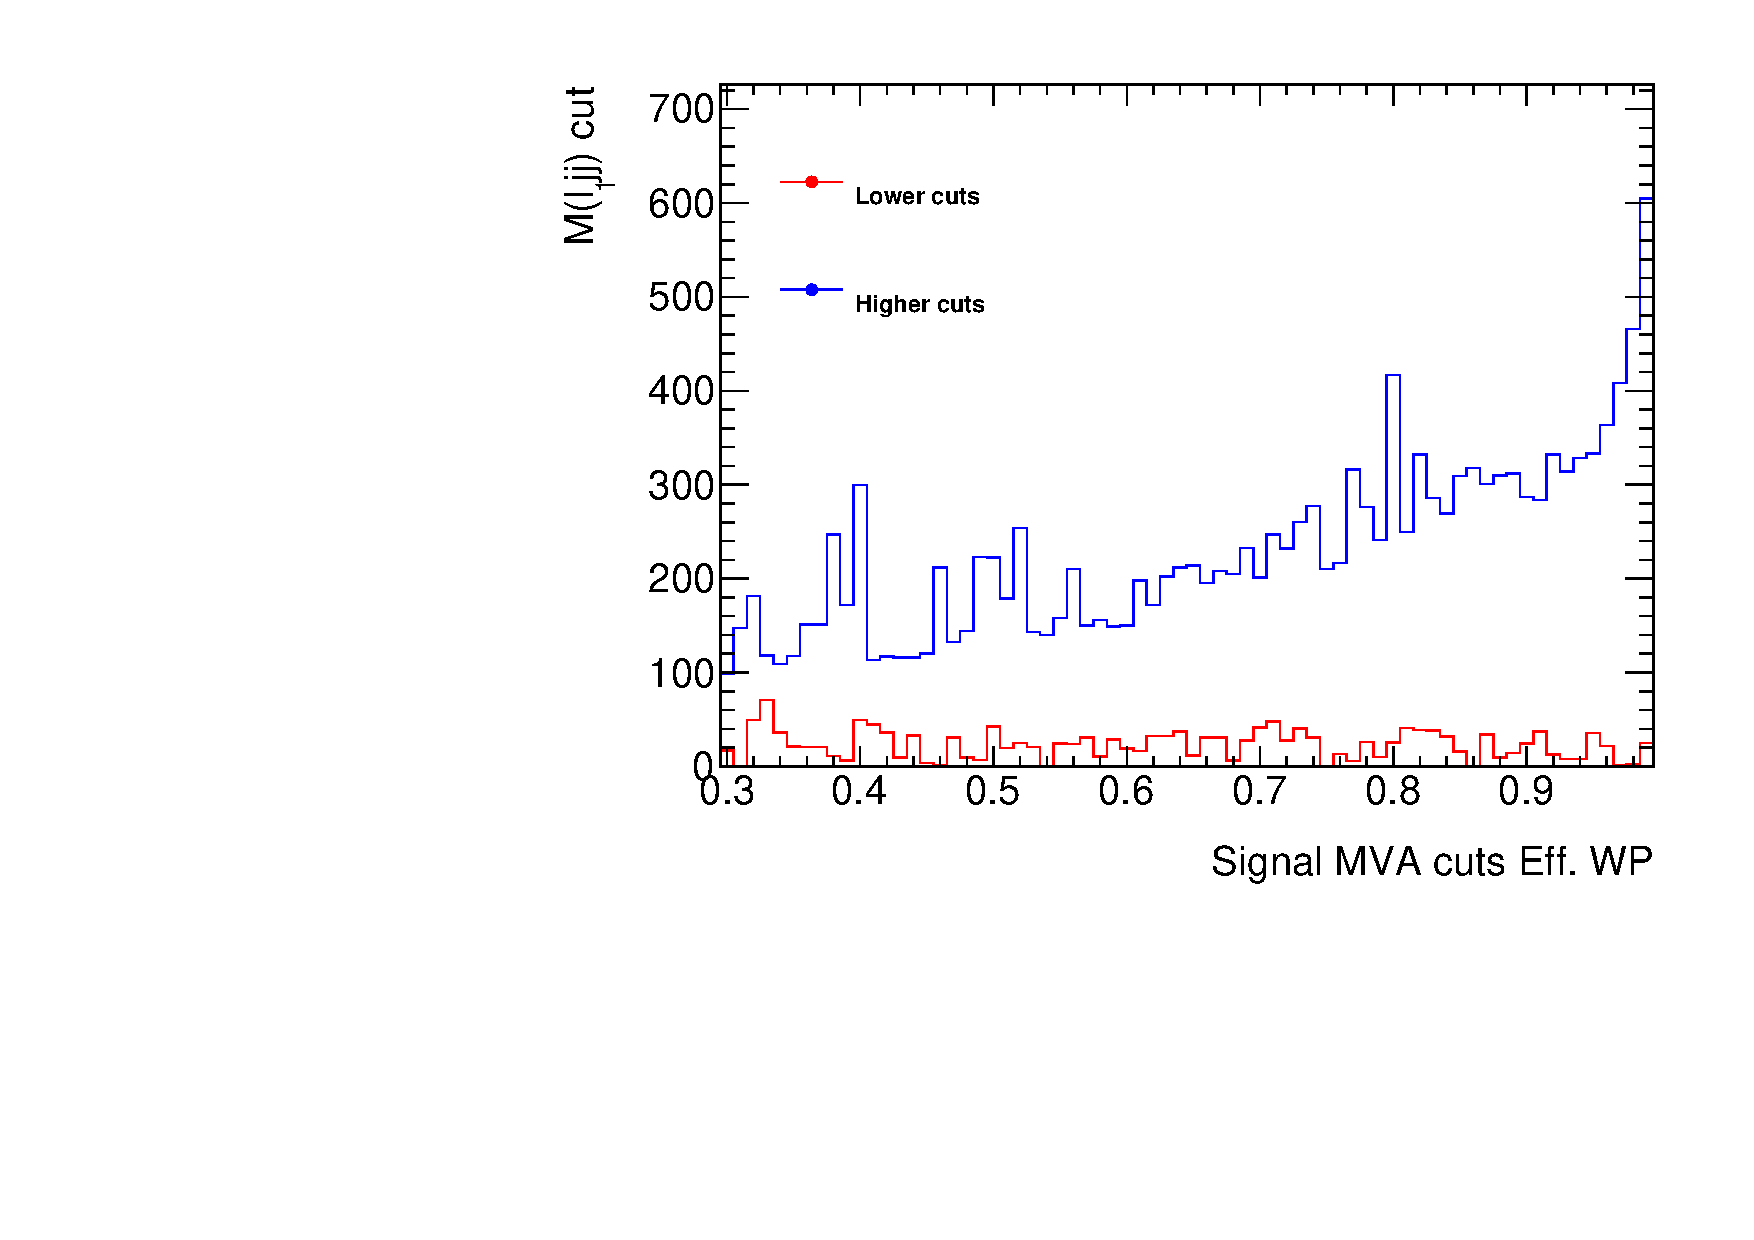
\includegraphics[width = 0.3\textwidth,angle=-90]{fig/SigOpt/nonres/m_l1jj_mumu.pdf}
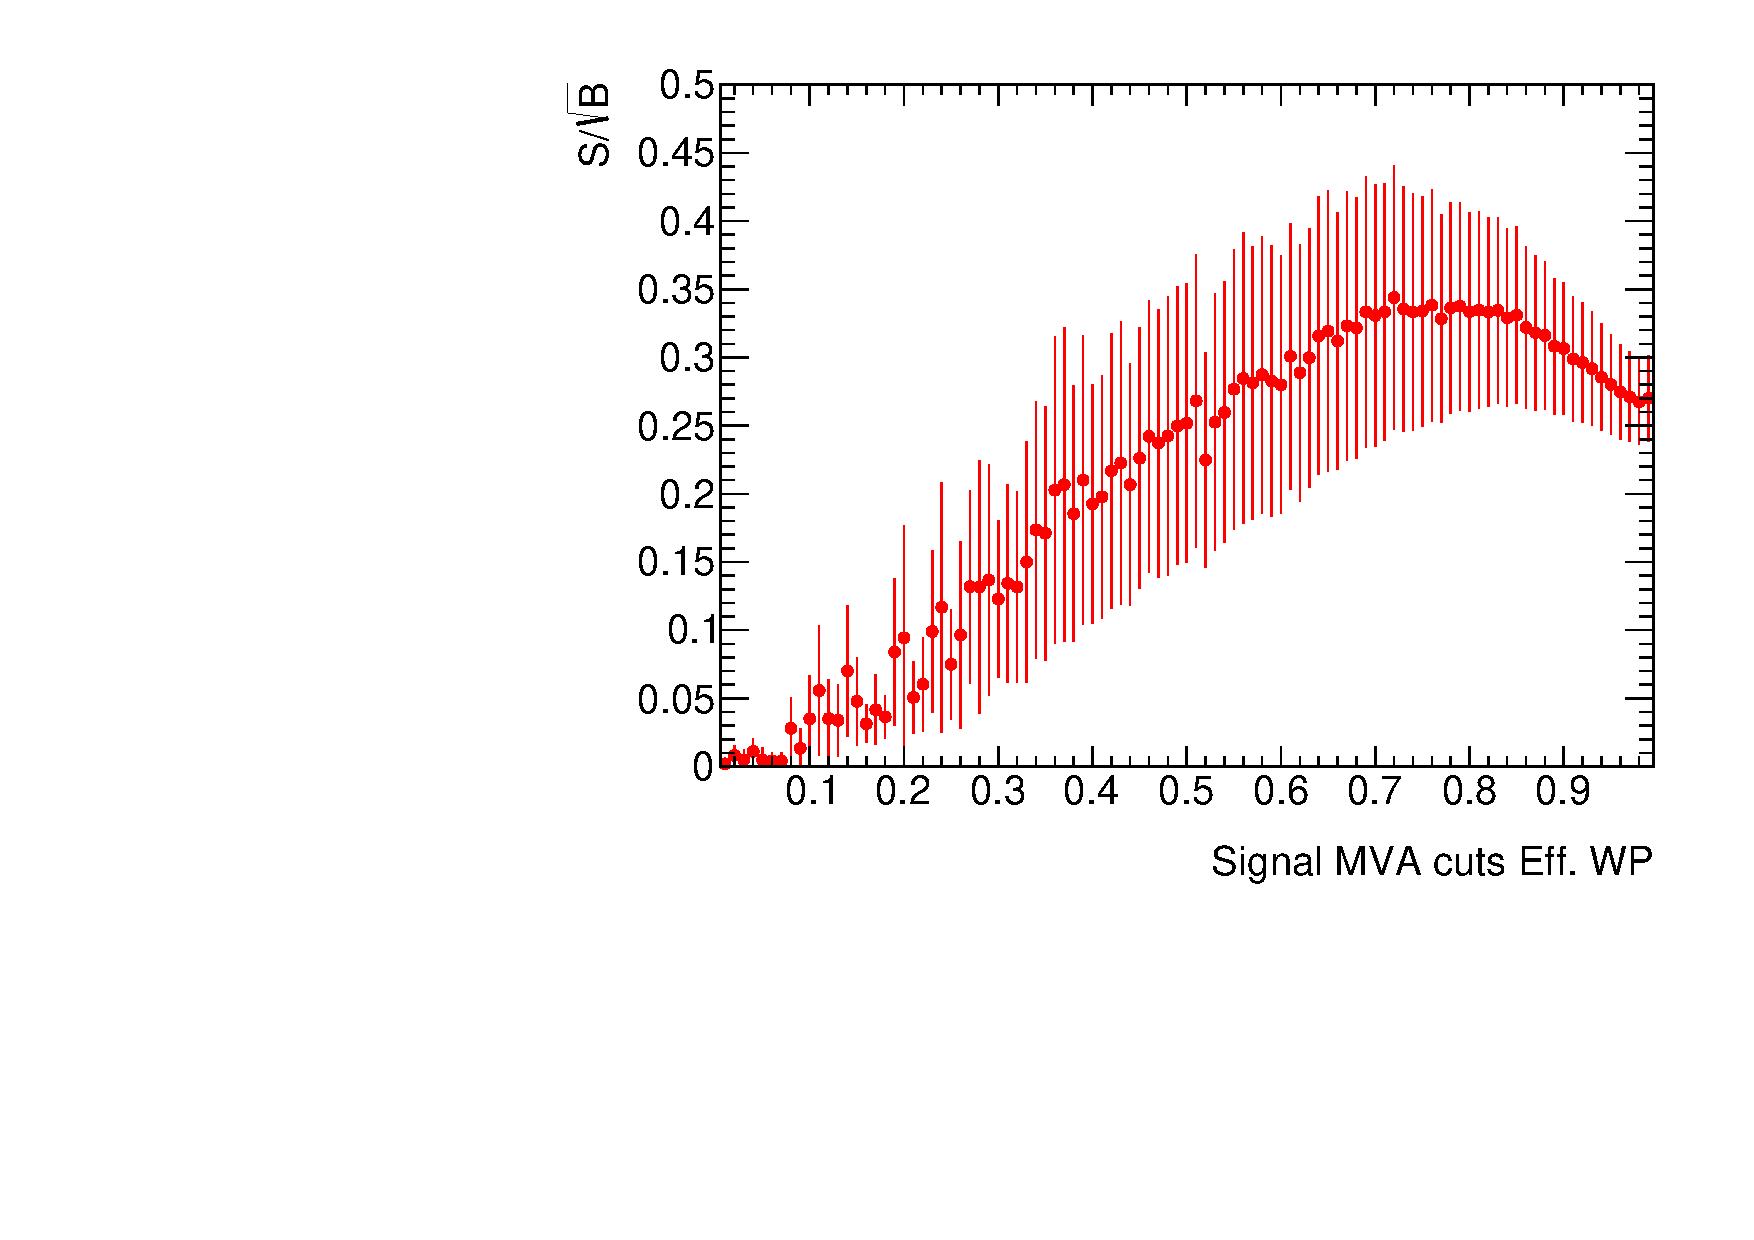
\includegraphics[width = 0.3\textwidth,angle=-90]{fig/SigOpt/nonres/SOverRootB_mumu.pdf}
\caption{利用CutsSA方法优化SM $hh$~$\mu\mu$信号时显著性随给定效率分布情况。信号与本地均考虑了统计误差,0.72选作SM $hh$~$\mu\mu$的最佳工作点,其相应的运动学变量筛选值则
用作最终信号优化条件(会进行一定的平滑性选择)。}
%\caption{The significance scan as a function of efficiency for $\mu\mu$ in non-resonant signal search. Statistical uncertainties on the background and the signal are considered. The 0.72 working point is chosen for $\mu\mu$ channel in the non-resonant signal optimizations.}
\label{fig:nonres:SigOpt_mumu}
\end{center}
\end{figure}

\begin{table}[h]
\begin{center}
\begin{tabular}{c|c|c|c|c|c}
\hline
\hline
  &Channel &$\Delta R_{min}(\ell_{1}, j)$ &$M(ll)$  &$M_{\ell_{1}jj}$ &$M(all)$\\
\hline
\multirow{3}{2.0cm}{$m_X$=260 GeV} &$ee$  &0.35, 1.85
&$<$100
&$<$145
&$<$1100  \\
&$\mu\mu$
&0.25, 2.10
&$<$80
&$<$115
&$<$700 \\
&$e\mu$
&0.25, 1.80
&$<$85
&$<$135
&$<$650\\
\hline
\multirow{3}{2.0cm}{$m_X$=300 GeV} &$ee$
&0.35, 1.75
&$<$120
&$<$160
&$<$1400 \\
&$\mu\mu$
&0.20, 1.75
&$<$115
&$<$185
&$<$1000 \\
&$e\mu$
&0.20, 1.80
&$<$135
&$<$160
&$<$800 \\
\hline
\hline
\end{tabular}
\end{center}
\caption{基于运动学变量$X \rightarrow hh$信号优化总结,对应$m_{X}$=260, 300 GeV,所有不变质量单位为GeV。}
%\caption{Summary of optimization selections for the search of $X \rightarrow hh$ ($m_{X}$=260, 300 GeV). All mass cuts are in GeV.}
\label{optimization_cuts_lowmass}
\end{table}

\begin{table}[h]
\begin{center}
\begin{tabular}{c|c|c|c|c|c}
\hline
\hline
  &Channel &$\Delta R_{min}(\ell_{2}, j)$ &$\Delta R_{min}(\ell_{1}, j)$ &$M(ll)$  &$M_{\ell_{1}jj}$ \\
\hline
\multirow{3}{2.0cm}{$m_X$=400 GeV} &$ee$
&0.35, 1.50
&0.30, 1.25
&45, 235
&40, 285 \\
&$\mu\mu$
&0.20, 1.20
&0.20, 1.20
&40, 215
&30, 260 \\
&$e\mu$
&0.20, 1.50
&0.20, 1.05
&35, 195
&30, 235 \\
\hline
\multirow{3}{2.0cm}{$m_X$=500 GeV} &$ee$
&0.20, 1.15
&0.20, 1.15
&100, 270
&40, 285 \\
&$\mu\mu$
&0.20, 1.05
&0.20, 0.75
&60, 250
&30, 310 \\
&$e\mu$
&0.20, 1.00
&0.20, 0.80
&75, 250
&35, 350 \\
\hline
\multirow{3}{2.0cm}{Non-resonant} & $ee$
&0.20, 1.40
&0.20, 1.15
&55, 270
&40, 285 \\
&$\mu\mu$
&0.20, 1.05
&0.20, 0.75
&60, 250
&30, 310 \\
&$e\mu$
&0.20, 1.15
&0.20, 0.80
&75, 250
&35, 350 \\
\hline
\hline
\end{tabular}
\end{center}
\caption{基于运动学变量$X \rightarrow hh$信号优化总结,对应$m_{X}$=400, 500 GeV以及SM $hh$,所有不变质量单位为GeV。}
%\caption{Summary of optimization selections for the search of $X \rightarrow hh$($m_{X}$=400, 500 GeV and non-resonant). All mass cuts are in GeV.}
\label{optimization_cuts_highmass}
\end{table}
 
\begin{table}[h]
\begin{center}
\begin{tabular}{c|c|c|c|c|c}
\hline
\hline
  &Channel &$\Delta R_{min}(\ell_{2}, j)$ &$\Delta R_{min}(\ell_{1}, j)$ &$M(ll)$  &$M_{\ell_{1}jj}$ \\
%\hline
%\multirow{3}{1.5cm}{mX=280 GeV, mS=135 GeV} &$ee$
%0.2 2.5
%0.2 1.7
%15 70
%40 125 \\
%&$\mu\mu$
%0.2 2
%0.25 1.65
%15 90
%0 130 \\
%&$e\mu$
%0.25 2.15
%0.2 1.7
%15 95
%0 120 \\
\hline
\multirow{3}{4.5cm}{$m_X$=300 GeV,$m_S$=135 GeV} &$ee$
&0.35, 2.5
&0.4, 1.65
& $<$80
&50, 150 \\
&$\mu\mu$
&0.25, 2.05
&0.2, 1.85
&$<$ 95
&50, 150 \\
&$e\mu$
&0.25, 1.7
&0.25, 1.65
&$<$ 95
&50, 150 \\
\hline
\multirow{3}{4.5cm}{$m_X$=340 GeV,$m_S$=145 GeV} &$ee$
&0.35, 1.85
&0.2, 1.65
&$<$ 130
&50, 190 \\
&$\mu\mu$
&0.2, 2.0
&0.2, 1.65
&$<$ 115
&50, 185 \\
&$e\mu$
&0.25, 1.6
&0.25, 1.6
&$<$ 150
&50, 150 \\
\hline
\hline
\end{tabular}
\end{center}
\caption{基于运动学变量$X \rightarrow SS$信号优化总结,所有不变质量单位为GeV。}
%\caption{Summary of optimization selections for the search of $X\rightarrow SS$. All mass cuts are in GeV.}
\label{optimization_cuts_HSS}
\end{table}

 
\clearpage
\subsection{优化效率检查}
为了防止过度优化或者欠优化的情况,可以检查每个信号MC经过以上选择条件之后的效率。
图~\ref {fig:eff_sigopt_hh}和图~\ref {fig:eff_sigopt_SS}分别表示$hh$和$SS$信号相对于经过初步筛选条件之后的选择效率。 总体上大多数质量点的选择效率相当接近,
 但是由于优化时每两个变量一组,它们之间的相关性在三个分析道中略有不同,并且各个分析道具有不同的背景组成,导致不同质量点不同分析道具有不同效率的趋势。
 \begin{figure}[h]
\begin{center}
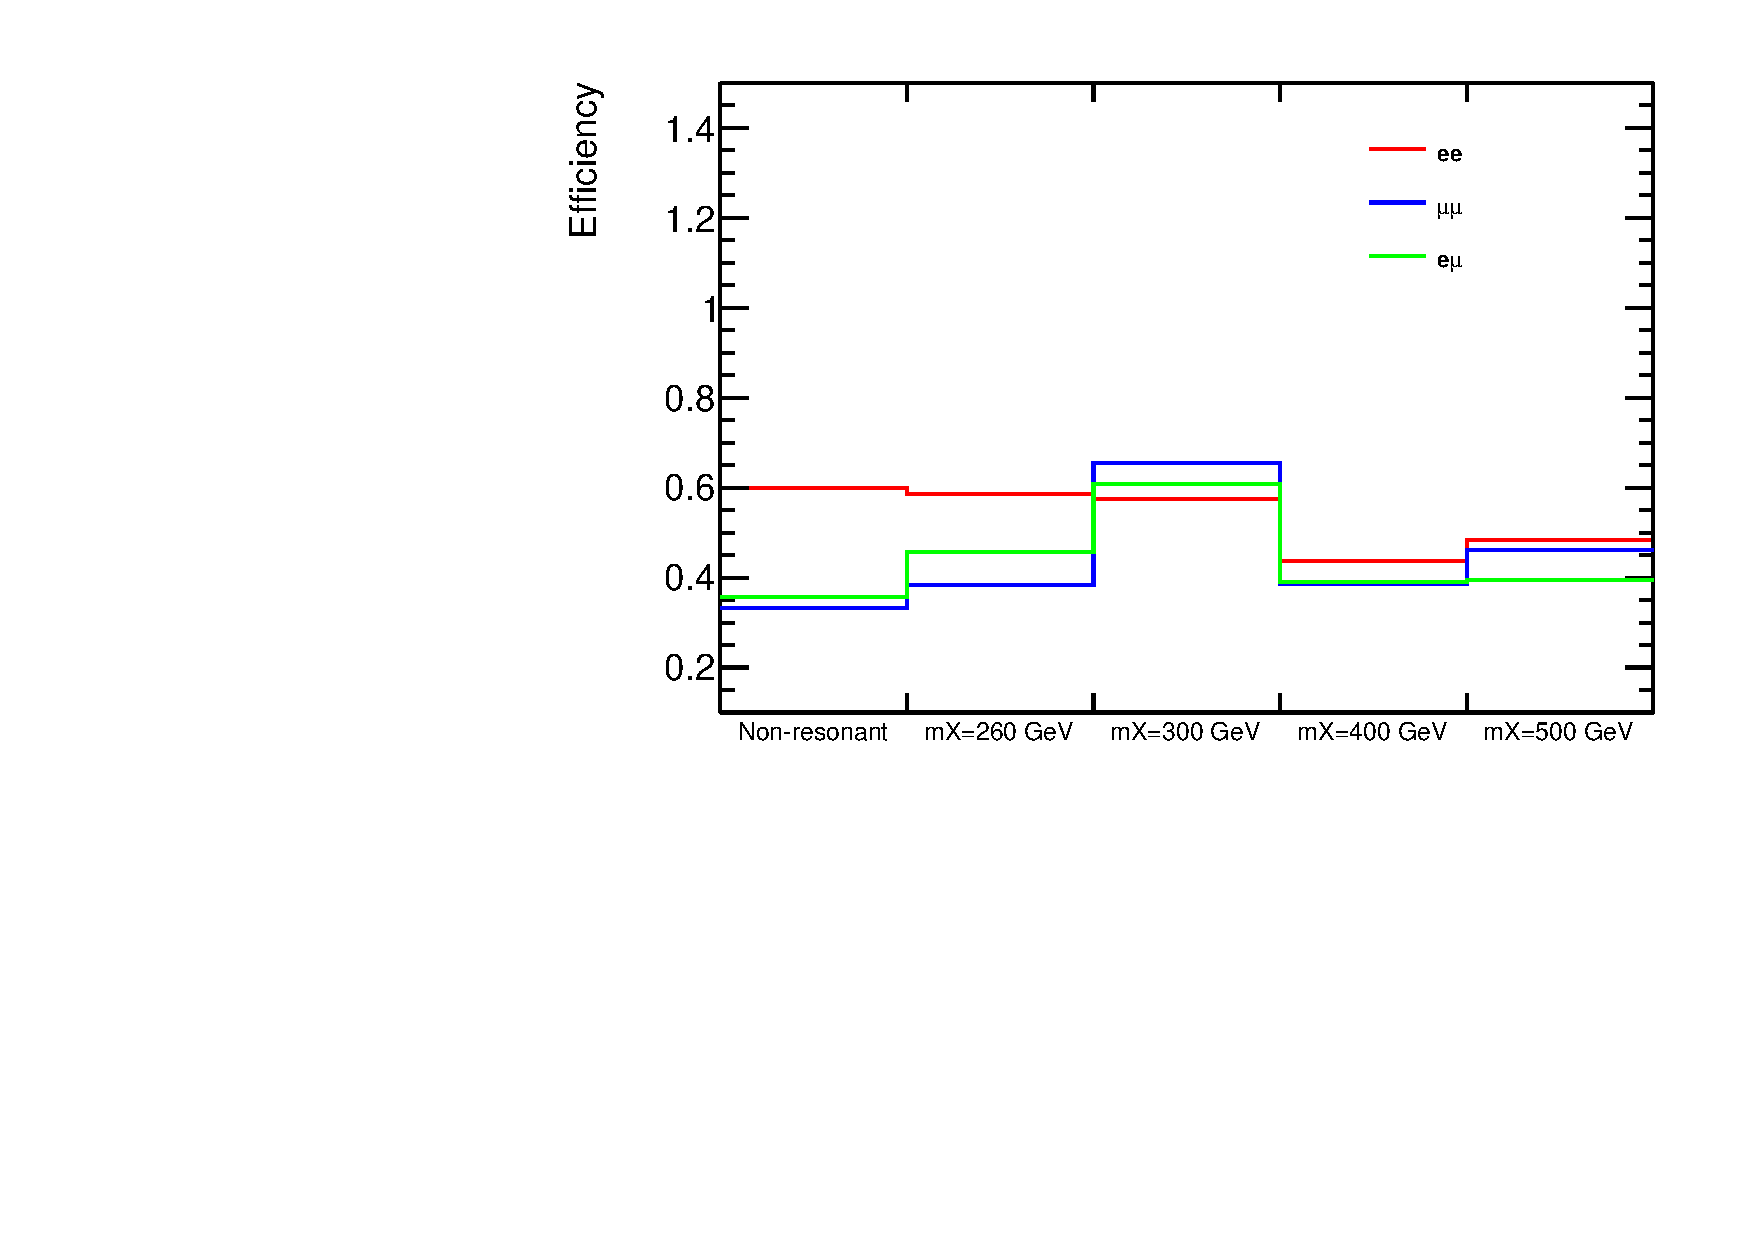
\includegraphics[width = 0.45\textwidth,angle=-90]{fig/SigOpt/eff_sigopt_hh.pdf}
\caption{$hh$信号优化效率(相比于初步筛选)。}
%\caption{Signal efficiency with respect to pre-selections in $ee$, $\mu\mu$ and $e\mu$ channel after applying all of the optimisation selections
%for the non-resonant and resonant $hh$ signal.}
\label{fig:eff_sigopt_hh}
\end{center}
\end{figure}

\begin{figure}[h]
\begin{center}
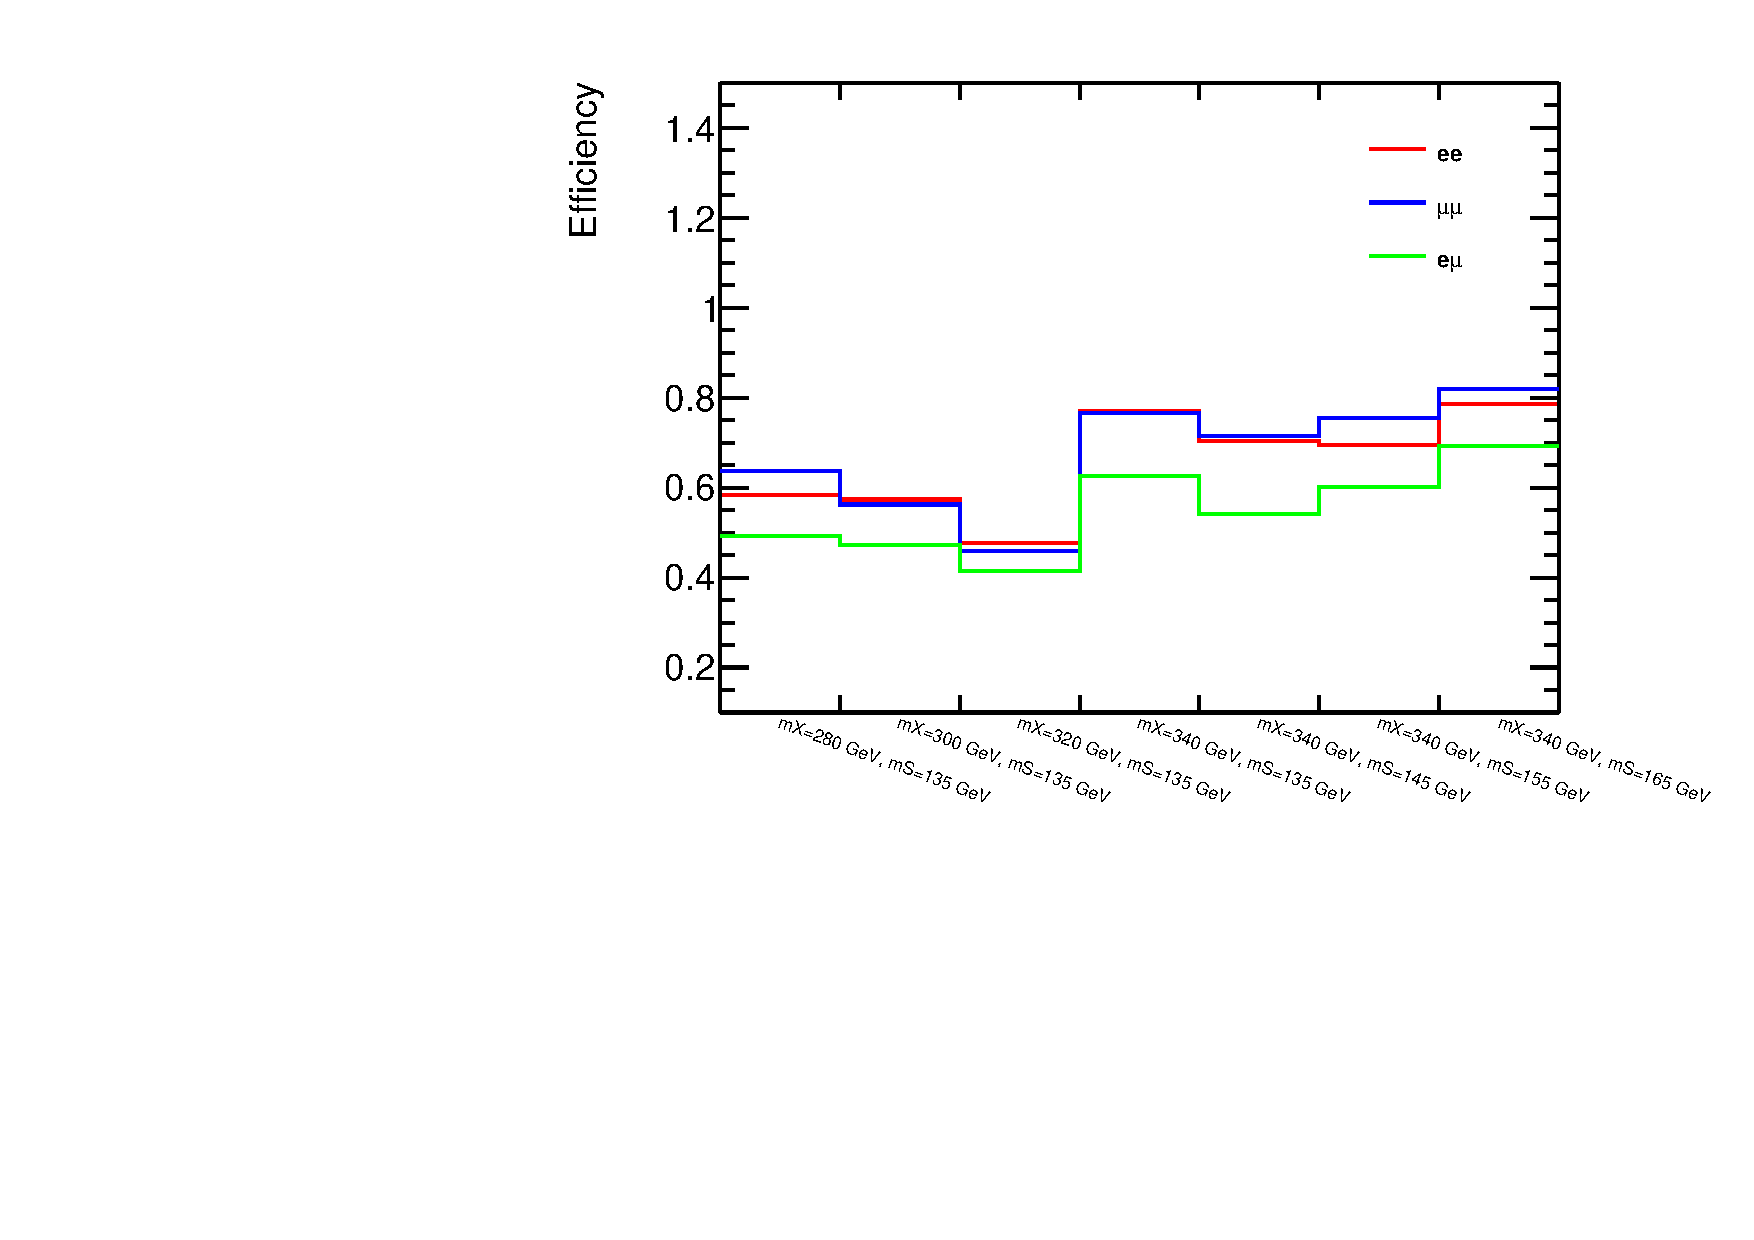
\includegraphics[width = 0.50\textwidth,angle=-90]{fig/SigOpt/eff_sigopt_SS.pdf}
\caption{$SS$信号优化效率(相比于初步筛选)。}
%\caption{Signal efficiency with respect to pre-selections in $ee$, $\mu\mu$ and $e\mu$ channel after applying all of the optimisation selections
%for the resonant $SS$ signal.}
\label{fig:eff_sigopt_SS}
\end{center}
\end{figure}

\clearpage
\subsection{优化结果}
\label{sec:unblind_results}
经过所有筛选条件之后,表~\ref{cutflow_ee_nonres}到表~\ref{cutflow_emu_HSS_highmass}展示各个质量点不同分析道中的各种背景,预期信号以及观测事例数的结果。总预期本底的误差包括了所有
的系统误差,并考虑了非fakes本底的系统误差(syst1)与fakes本底的系统误差(syst2)的反相关性质。对于每个质量点的每个分析道,一个运动学变量的分布也被展示,
从图~\ref{fig:SigOpt:nonres_m_l1jj.pdf}到图~\ref{fig:SigOpt:H340_S165_m_l1jj.pdf}。
\subsubsection{$hh$搜寻筛选结果}
\begin{table}[h]
\begin{center}
\tiny\scalebox{0.8}{
\begin{tabular}{c|cccc|cc|c}
\hline
\hline
                           &promptSS  &$V+\gamma$  &QmisID  &Fakes  &Total bkg  &Observed  &signal  \\  
\hline
$\Delta R_{min}(l_{2},j)$ &46.87$\pm$2.91(stat.)$\pm$14.06(syst.)  &16.25$\pm$3.99(stat.)$\pm$8.12(syst.)  &15.60$\pm$0.24(stat.)$\pm$5.15(syst.)  &64.87$\pm$5.96(stat.)$\pm$44.88(syst.)  &143.59$\pm$7.74(stat.)$\mp$17.04(syst1.)$\pm$44.88(syst2.)  &158  &0.04$\pm$0.00\\
\hline
$\Delta R_{min}(l_{1},j)$ &16.38$\pm$1.80(stat.)$\pm$4.91(syst.)  &2.89$\pm$1.04(stat.)$\pm$1.45(syst.)  &5.23$\pm$0.13(stat.)$\pm$1.72(syst.)  &26.32$\pm$3.79(stat.)$\pm$18.21(syst.)  &50.81$\pm$4.33(stat.)$\mp$5.40(syst1.)$\pm$18.21(syst2.)  &62  &0.03$\pm$0.00\\
\hline
$M(\ell\ell)$ &11.70$\pm$1.65(stat.)$\pm$3.51(syst.)  &0.95$\pm$0.34(stat.)$\pm$0.48(syst.)  &3.38$\pm$0.10(stat.)$\pm$1.12(syst.)  &21.24$\pm$3.41(stat.)$\pm$14.70(syst.)  &37.28$\pm$3.80(stat.)$\mp$3.72(syst1.)$\pm$14.70(syst2.)  &46  &0.03$\pm$0.00\\
\hline
$M(l_{1}jj)$ &8.37$\pm$1.04(stat.)$\pm$2.51(syst.)  &0.54$\pm$0.24(stat.)$\pm$0.27(syst.)  &2.61$\pm$0.09(stat.)$\pm$0.86(syst.)  &17.46$\pm$3.09(stat.)$\pm$12.08(syst.)  &28.98$\pm$3.27(stat.)$\mp$2.67(syst1.)$\pm$12.08(syst2.)  &35  &0.03$\pm$0.00\\
\hline
\hline
\end{tabular}}
\end{center}

\caption{SM $hh$ $ee$类别的优化结果。 }
\label{cutflow_ee_nonres}
\end{table}

\begin{table}[h]
\begin{center}
\tiny\scalebox{0.65}{
\begin{tabular}{c|cccc|cc|c}
\hline
\hline
                           &promptSS  &$V+\gamma$  &QmisID  &Fakes  &Total bkg  &Observed  &signal  \\  
\hline
$\Delta R_{min}(l_{2},j)$ &47.41$\pm$2.70(stat.)$\pm$14.22(syst.)  &0.01$\pm$0.01(stat.)$\pm$0.00(syst.)  &0.00$\pm$0.00(stat.)$\pm$0.00(syst.)  &37.76$\pm$4.14(stat.)$\pm$27.11(syst.)  &85.17$\pm$4.94(stat.)$\mp$14.22(syst1.)$\pm$27.11(syst2.)  &72  &0.07$\pm$0.00\\
\hline
$\Delta R_{min}(l_{1},j)$ &9.52$\pm$1.17(stat.)$\pm$2.86(syst.)  &0.00$\pm$0.00(stat.)$\pm$0.00(syst.)  &0.00$\pm$0.00(stat.)$\pm$0.00(syst.)  &5.59$\pm$1.59(stat.)$\pm$4.01(syst.)  &15.11$\pm$1.98(stat.)$\mp$2.86(syst1.)$\pm$4.01(syst2.)  &10  &0.04$\pm$0.00\\
\hline
$M(\ell\ell)$ &6.21$\pm$0.97(stat.)$\pm$1.86(syst.)  &0.00$\pm$0.00(stat.)$\pm$0.00(syst.)  &0.00$\pm$0.00(stat.)$\pm$0.00(syst.)  &4.01$\pm$1.35(stat.)$\pm$2.88(syst.)  &10.22$\pm$1.66(stat.)$\mp$1.86(syst1.)$\pm$2.88(syst2.)  &4  &0.04$\pm$0.00\\
\hline
$M(l_{1}jj)$ &4.50$\pm$0.74(stat.)$\pm$1.35(syst.)  &0.00$\pm$0.00(stat.)$\pm$0.00(syst.)  &0.00$\pm$0.00(stat.)$\pm$0.00(syst.)  &3.56$\pm$1.27(stat.)$\pm$2.55(syst.)  &8.05$\pm$1.47(stat.)$\mp$1.35(syst1.)$\pm$2.55(syst2.)  &4  &0.03$\pm$0.00\\
\hline
\hline
\end{tabular}}
\end{center}

\caption{SM $hh$ $\mu\mu$类别的优化结果。}
%\caption{The unblinded results of non-resonant search in $\mu\mu$ channel. }
\label{cutflow_mumu_nonres}
\end{table}

\begin{table}[h]
\begin{center}
\tiny\scalebox{0.65}{
\begin{tabular}{c|cccc|cc|c}
\hline
\hline
                           &promptSS  &$V+\gamma$  &QmisID  &Fakes  &Total bkg  &Observed  &signal  \\  
\hline
$\Delta R_{min}(l_{2},j)$ &94.91$\pm$3.97(stat.)$\pm$28.47(syst.)  &15.89$\pm$4.14(stat.)$\pm$7.95(syst.)  &3.46$\pm$0.11(stat.)$\pm$1.14(syst.)  &48.27$\pm$4.96(stat.)$\pm$24.35(syst.)  &162.53$\pm$7.59(stat.)$\mp$29.58(syst1.)$\pm$24.35(syst2.)  &194  &0.11$\pm$0.00\\
\hline
$\Delta R_{min}(l_{1},j)$ &19.61$\pm$1.80(stat.)$\pm$5.88(syst.)  &1.88$\pm$0.94(stat.)$\pm$0.94(syst.)  &0.68$\pm$0.05(stat.)$\pm$0.22(syst.)  &9.16$\pm$2.20(stat.)$\pm$5.30(syst.)  &31.33$\pm$2.99(stat.)$\mp$5.96(syst1.)$\pm$5.30(syst2.)  &44  &0.06$\pm$0.00\\
\hline
$M(\ell\ell)$ &11.34$\pm$1.29(stat.)$\pm$3.40(syst.)  &0.24$\pm$0.21(stat.)$\pm$0.12(syst.)  &0.34$\pm$0.03(stat.)$\pm$0.11(syst.)  &1.73$\pm$0.94(stat.)$\pm$0.89(syst.)  &13.65$\pm$1.61(stat.)$\mp$3.41(syst1.)$\pm$0.89(syst2.)  &21  &0.05$\pm$0.00\\
\hline
$M(l_{1}jj)$ &9.28$\pm$1.15(stat.)$\pm$2.79(syst.)  &0.24$\pm$0.21(stat.)$\pm$0.12(syst.)  &0.27$\pm$0.03(stat.)$\pm$0.09(syst.)  &1.33$\pm$0.82(stat.)$\pm$0.66(syst.)  &11.13$\pm$1.43(stat.)$\mp$2.79(syst1.)$\pm$0.66(syst2.)  &18  &0.05$\pm$0.00\\
\hline
\hline
\end{tabular}}
\end{center}

\caption{SM $hh$ $e\mu$类别的优化结果。}
%\caption{The unblinded results of non-resonant search in $e\mu$ channel. }
\label{cutflow_emu_nonres}
\end{table}

\begin{figure}[h]
\begin{minipage}[t]{0.33\linewidth}
 \centering
 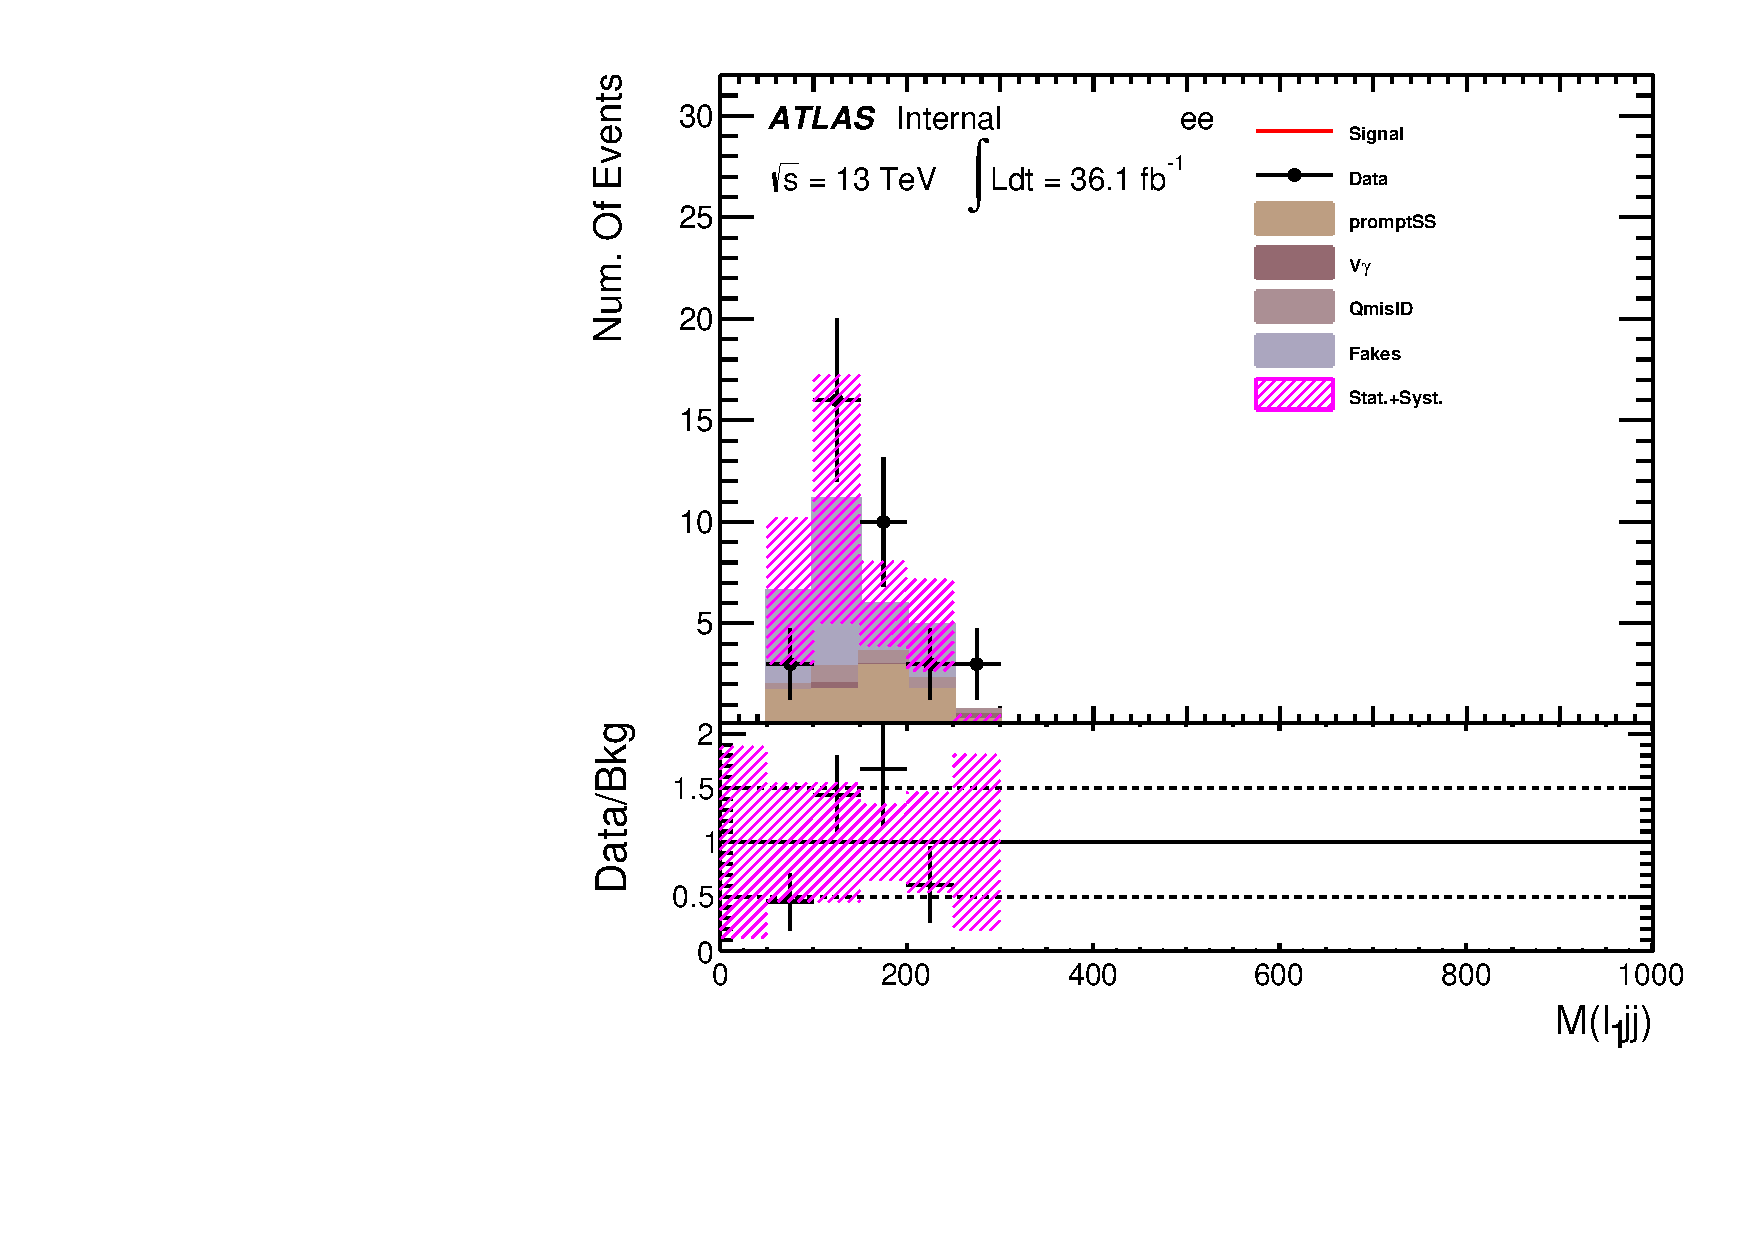
\includegraphics[width=0.9\textwidth,angle=-90]{fig/SigOpt/nonres_m_l1jj_ee.pdf}
 \end{minipage}
 \begin{minipage}[t]{0.33\linewidth}
 \centering
 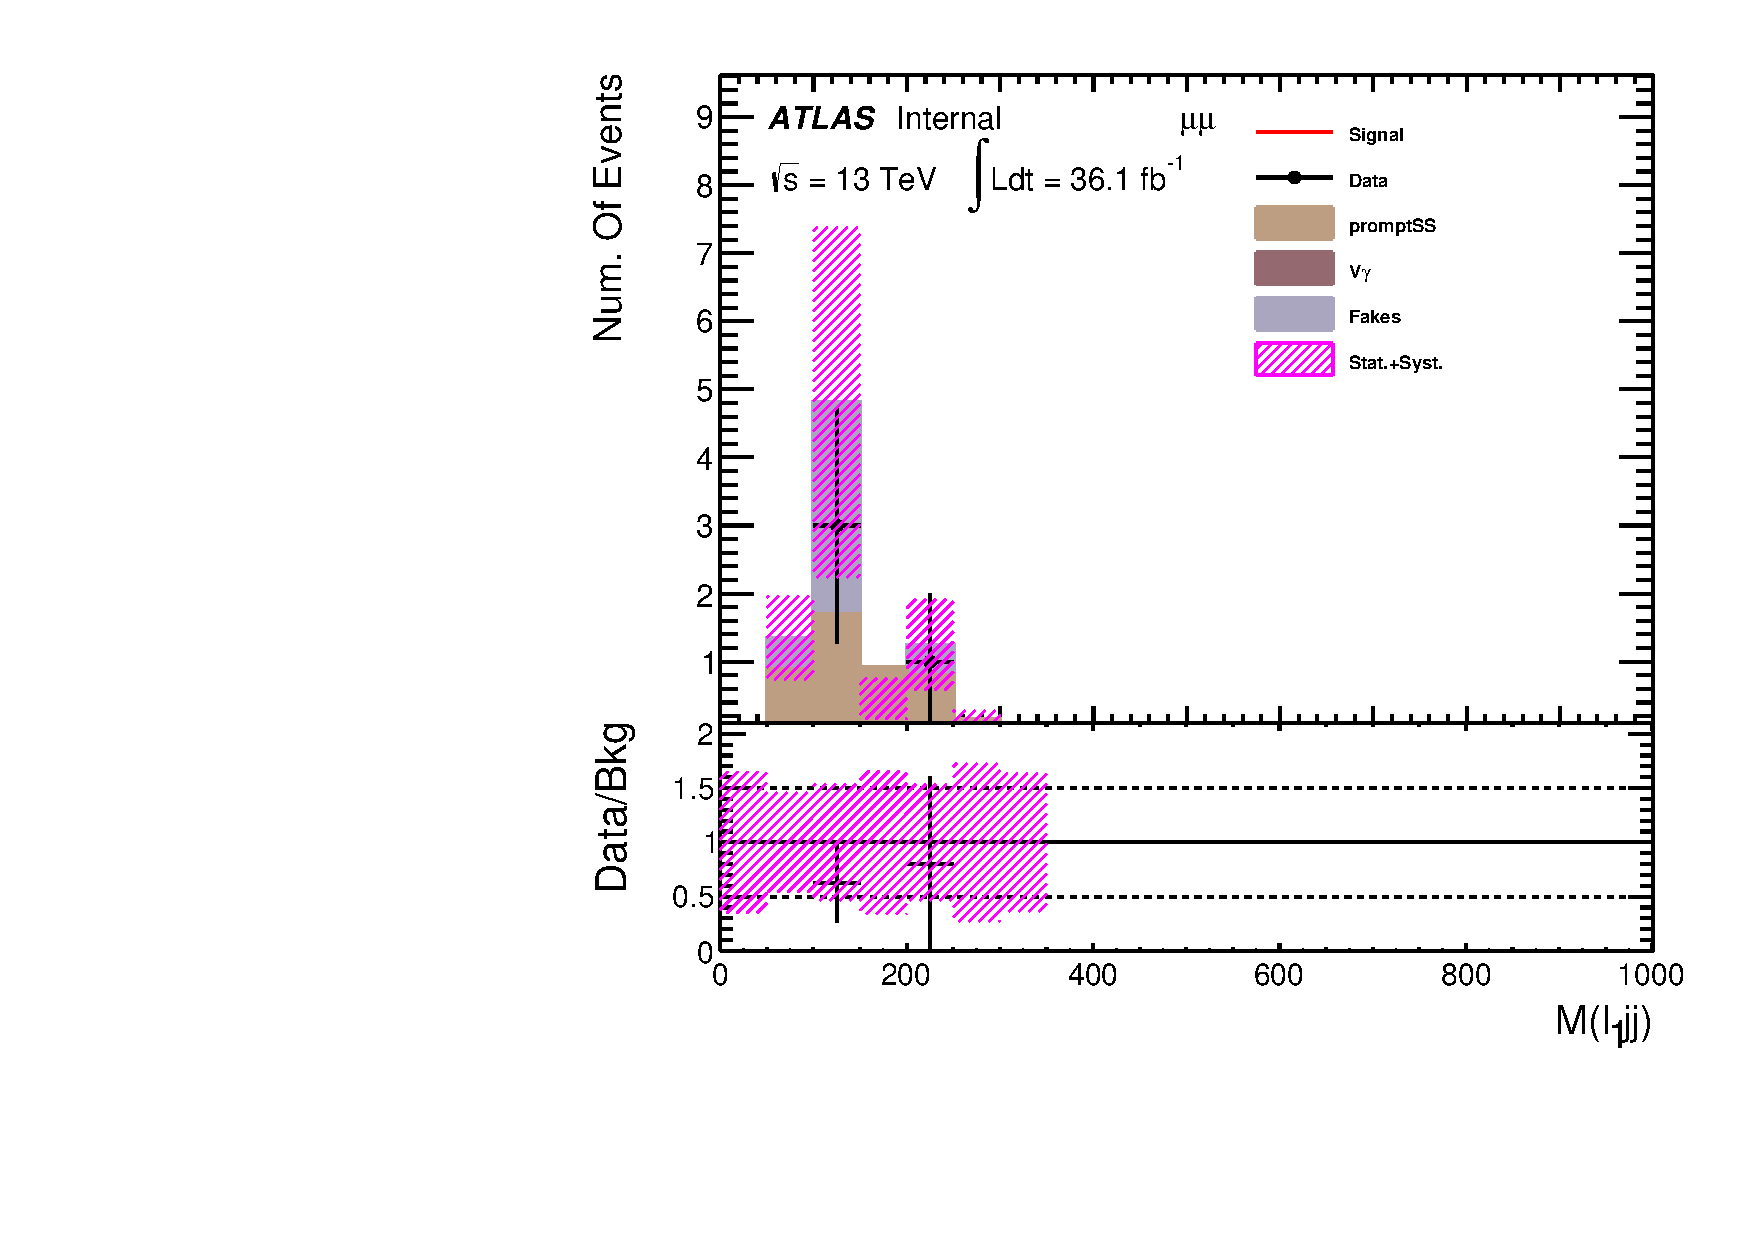
\includegraphics[width=0.9\textwidth,angle=-90]{fig/SigOpt/nonres_m_l1jj_mumu.pdf}
 \end{minipage}
 \begin{minipage}[t]{0.33\linewidth}
 \centering
 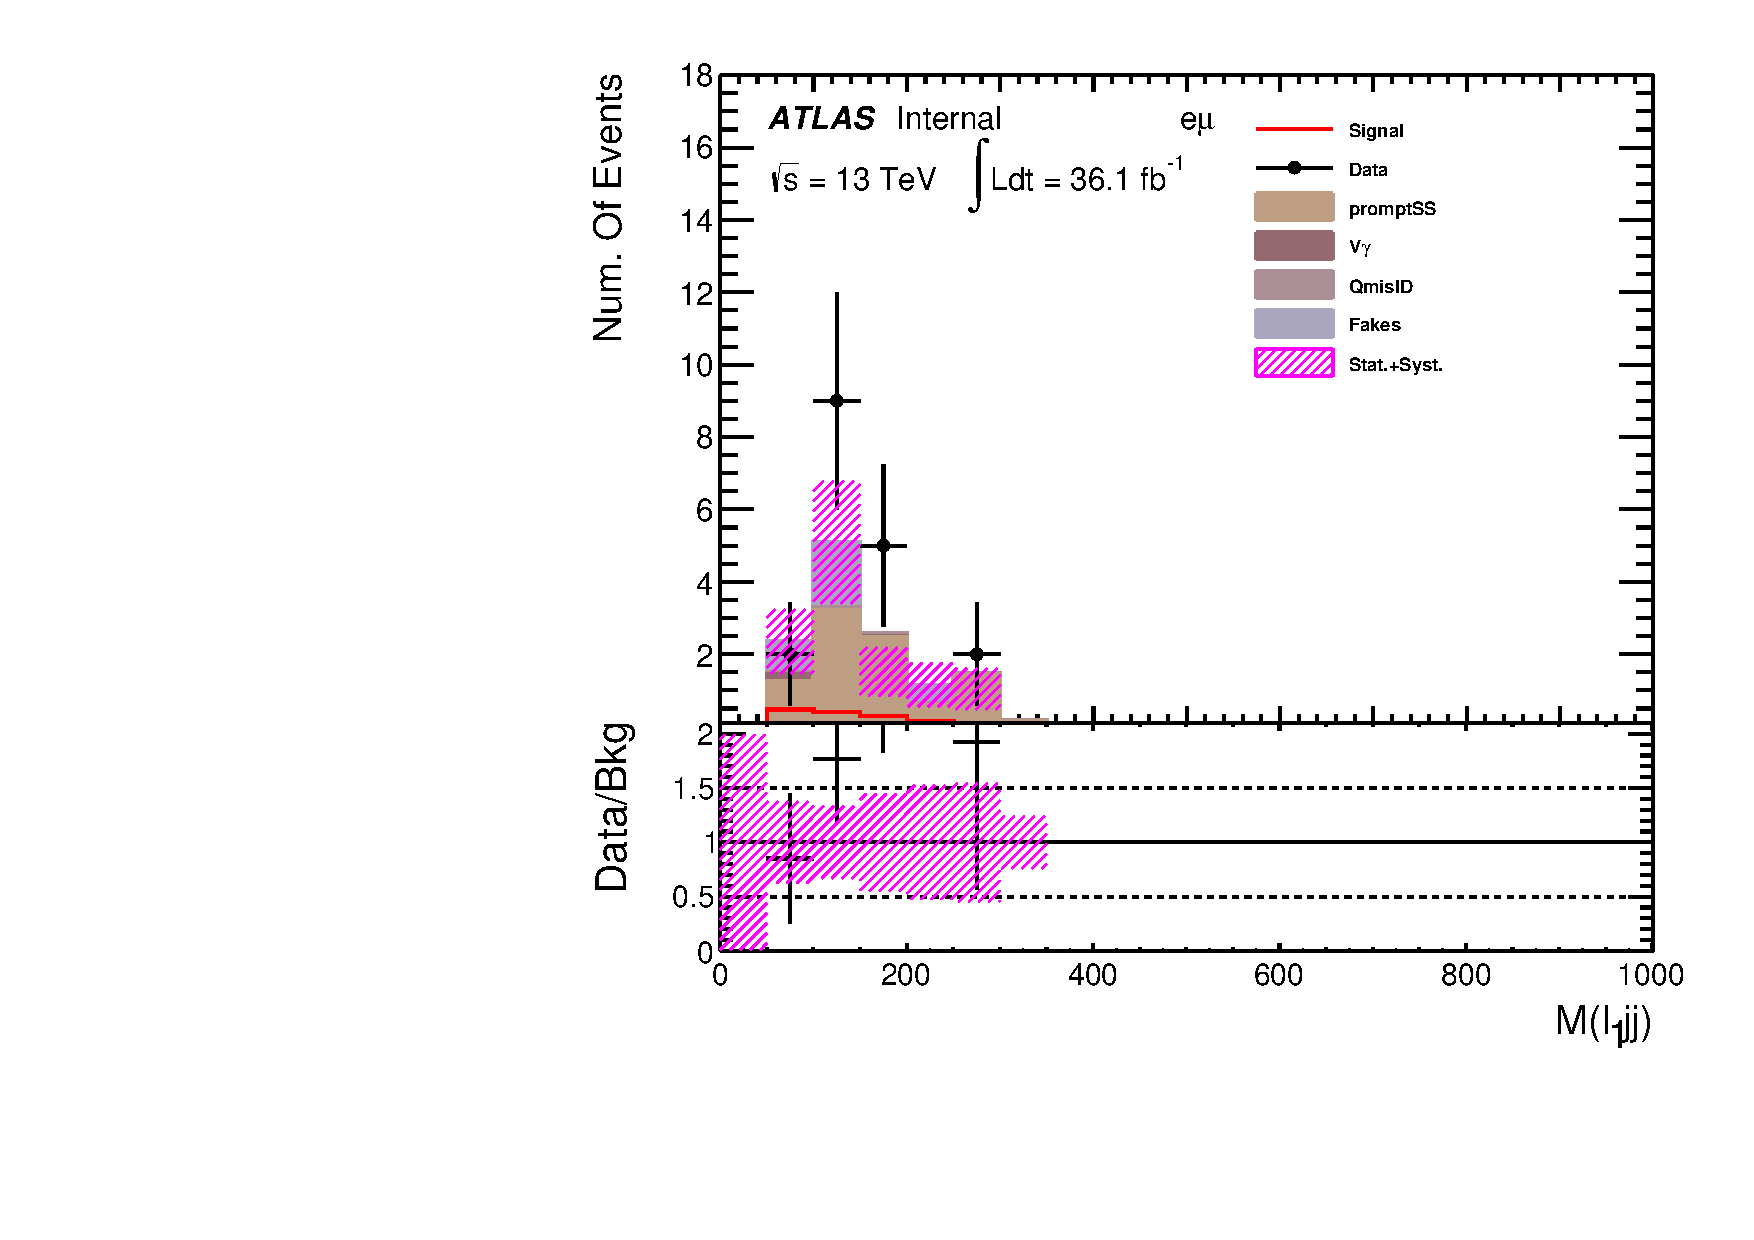
\includegraphics[width=0.9\textwidth,angle=-90]{fig/SigOpt/nonres_m_l1jj_emu.pdf}
 \end{minipage}
 \caption{SM hh质量点经过优化筛选之后$M(\ell_{1}jj)$分布。}
%\caption{The unblinded $M(\ell_{1}jj)$ distribution after all optimization selections, corresponding to non-resonance search.}
\label{fig:SigOpt:nonres_m_l1jj.pdf}
\end{figure}

\begin{table}[h]
\begin{center}
\tiny\scalebox{0.65}{
\begin{tabular}{c|cccc|cc|c}
\hline
\hline
                          &promptSS  &$V+\gamma$  &QmisID  &Fakes  &Total bkg  &Observed  &signal  \\
\hline
$\Delta R_{min}(l_{2},j)$ &110.96$\pm$4.65(stat.)$\pm$33.29(syst.)  &37.23$\pm$6.02(stat.)$\pm$18.61(syst.)  &39.43$\pm$0.35(stat.)$\pm$13.01(syst.)  &145.41$\pm$8.86(stat.)$\pm$91.74(syst.)  &333.03$\pm$11.69(stat.)$\mp$40.30(syst1.)$\pm$91.74(syst2.)  &371  &0.59$\pm$0.03\\
\hline
$\Delta R_{min}(l_{1},j)$ &39.91$\pm$2.89(stat.)$\pm$11.97(syst.)  &21.34$\pm$4.74(stat.)$\pm$10.67(syst.)  &17.43$\pm$0.18(stat.)$\pm$5.75(syst.)  &86.67$\pm$6.84(stat.)$\pm$54.68(syst.)  &165.35$\pm$8.81(stat.)$\mp$17.04(syst1.)$\pm$54.68(syst2.)  &173  &0.58$\pm$0.03\\
\hline
$M(\ell\ell)$ &12.41$\pm$1.74(stat.)$\pm$3.72(syst.)  &3.34$\pm$1.26(stat.)$\pm$1.67(syst.)  &4.78$\pm$0.06(stat.)$\pm$1.58(syst.)  &28.20$\pm$3.90(stat.)$\pm$17.79(syst.)  &48.72$\pm$4.45(stat.)$\mp$4.37(syst1.)$\pm$17.79(syst2.)  &63  &0.44$\pm$0.03\\
\hline
$M(l_{1}jj)$ &11.71$\pm$1.71(stat.)$\pm$3.51(syst.)  &3.34$\pm$1.26(stat.)$\pm$1.67(syst.)  &4.68$\pm$0.06(stat.)$\pm$1.55(syst.)  &27.96$\pm$3.89(stat.)$\pm$17.64(syst.)  &47.70$\pm$4.43(stat.)$\mp$4.19(syst1.)$\pm$17.64(syst2.)  &62  &0.44$\pm$0.02\\
\hline
\hline
\end{tabular}}
\end{center}

\caption{$m_X$=260~GeV $ee$类别的优化结果。}
%\caption{The unblinded results of $m_X$=260~GeV search in $ee$ channel. }
\label{cutflow_ee_mX260}
\end{table}

\begin{table}[h]
\begin{center}
\tiny\scalebox{0.65}{
\begin{tabular}{c|cccc|cc|c}
\hline
\hline
                          &promptSS  &$V+\gamma$  &QmisID  &Fakes  &Total bkg  &Observed  &signal  \\
\hline
$\Delta R_{min}(l_{2},j)$ &207.37$\pm$6.74(stat.)$\pm$62.21(syst.)  &0.01$\pm$0.01(stat.)$\pm$0.00(syst.)  &0.00$\pm$0.00(stat.)$\pm$0.00(syst.)  &181.81$\pm$9.57(stat.)$\pm$117.36(syst.)  &389.18$\pm$11.70(stat.)$\mp$62.21(syst1.)$\pm$117.36(syst2.)  &309  &1.21$\pm$0.04\\
\hline
$\Delta R_{min}(l_{1},j)$ &73.92$\pm$4.34(stat.)$\pm$22.18(syst.)  &0.00$\pm$0.00(stat.)$\pm$0.00(syst.)  &0.00$\pm$0.00(stat.)$\pm$0.00(syst.)  &91.31$\pm$6.78(stat.)$\pm$58.94(syst.)  &165.23$\pm$8.05(stat.)$\mp$22.18(syst1.)$\pm$58.94(syst2.)  &102  &1.07$\pm$0.04\\
\hline
$M(\ell\ell)$ &10.34$\pm$1.52(stat.)$\pm$3.10(syst.)  &0.00$\pm$0.00(stat.)$\pm$0.00(syst.)  &0.00$\pm$0.00(stat.)$\pm$0.00(syst.)  &17.80$\pm$2.99(stat.)$\pm$11.49(syst.)  &28.13$\pm$3.36(stat.)$\mp$3.10(syst1.)$\pm$11.49(syst2.)  &20  &0.56$\pm$0.03\\
\hline
$M(l_{1}jj)$ &8.79$\pm$1.47(stat.)$\pm$2.64(syst.)  &0.00$\pm$0.00(stat.)$\pm$0.00(syst.)  &0.00$\pm$0.00(stat.)$\pm$0.00(syst.)  &14.91$\pm$2.74(stat.)$\pm$9.63(syst.)  &23.70$\pm$3.11(stat.)$\mp$2.64(syst1.)$\pm$9.63(syst2.)  &17  &0.54$\pm$0.03\\
\hline
\hline
\end{tabular}}
\end{center}

\caption{$m_X$=260~GeV $\mu\mu$类别的优化结果。}
%\caption{The unblinded results of $m_X$=260~GeV search in $\mu\mu$ channel. }
\label{cutflow_mumu_mX260}
\end{table}

\begin{table}[h]
\begin{center}
\tiny\scalebox{0.8}{
\begin{tabular}{c|cccc|cc|c}
\hline
\hline
                          &promptSS  &$V+\gamma$  &QmisID  &Fakes  &Total bkg  &Observed  &signal  \\
\hline
$\Delta R_{min}(l_{2},j)$ &282.43$\pm$7.10(stat.)$\pm$84.73(syst.)  &36.01$\pm$5.38(stat.)$\pm$18.00(syst.)  &9.42$\pm$0.16(stat.)$\pm$3.11(syst.)  &169.37$\pm$9.45(stat.)$\pm$78.88(syst.)  &497.22$\pm$12.99(stat.)$\mp$86.67(syst1.)$\pm$78.88(syst2.)  &589  &1.69$\pm$0.05\\
\hline
$\Delta R_{min}(l_{1},j)$ &105.47$\pm$4.54(stat.)$\pm$31.64(syst.)  &18.73$\pm$4.47(stat.)$\pm$9.37(syst.)  &2.02$\pm$0.04(stat.)$\pm$0.67(syst.)  &103.33$\pm$7.37(stat.)$\pm$47.60(syst.)  &229.55$\pm$9.74(stat.)$\mp$33.00(syst1.)$\pm$47.60(syst2.)  &244  &1.53$\pm$0.05\\
\hline
$M(\ell\ell)$ &29.17$\pm$2.42(stat.)$\pm$8.75(syst.)  &5.89$\pm$1.87(stat.)$\pm$2.95(syst.)  &0.54$\pm$0.02(stat.)$\pm$0.18(syst.)  &45.62$\pm$4.90(stat.)$\pm$20.94(syst.)  &81.23$\pm$5.77(stat.)$\mp$9.23(syst1.)$\pm$20.94(syst2.)  &80  &1.04$\pm$0.04\\
\hline
$M(l_{1}jj)$ &23.61$\pm$2.14(stat.)$\pm$7.08(syst.)  &4.87$\pm$1.67(stat.)$\pm$2.44(syst.)  &0.46$\pm$0.01(stat.)$\pm$0.15(syst.)  &41.89$\pm$4.69(stat.)$\pm$19.28(syst.)  &70.84$\pm$5.42(stat.)$\mp$7.49(syst1.)$\pm$19.28(syst2.)  &70  &0.99$\pm$0.04\\
\hline
\hline
\end{tabular}}
\end{center}

\caption{$m_X$=260~GeV $e\mu$类别的优化结果。}
%\caption{The unblinded results of $m_X$=260~GeV search in $e\mu$ channel. }
\label{cutflow_emu_mX260}
\end{table}

\begin{figure}[h]
\begin{minipage}[t]{0.33\linewidth}
 \centering
 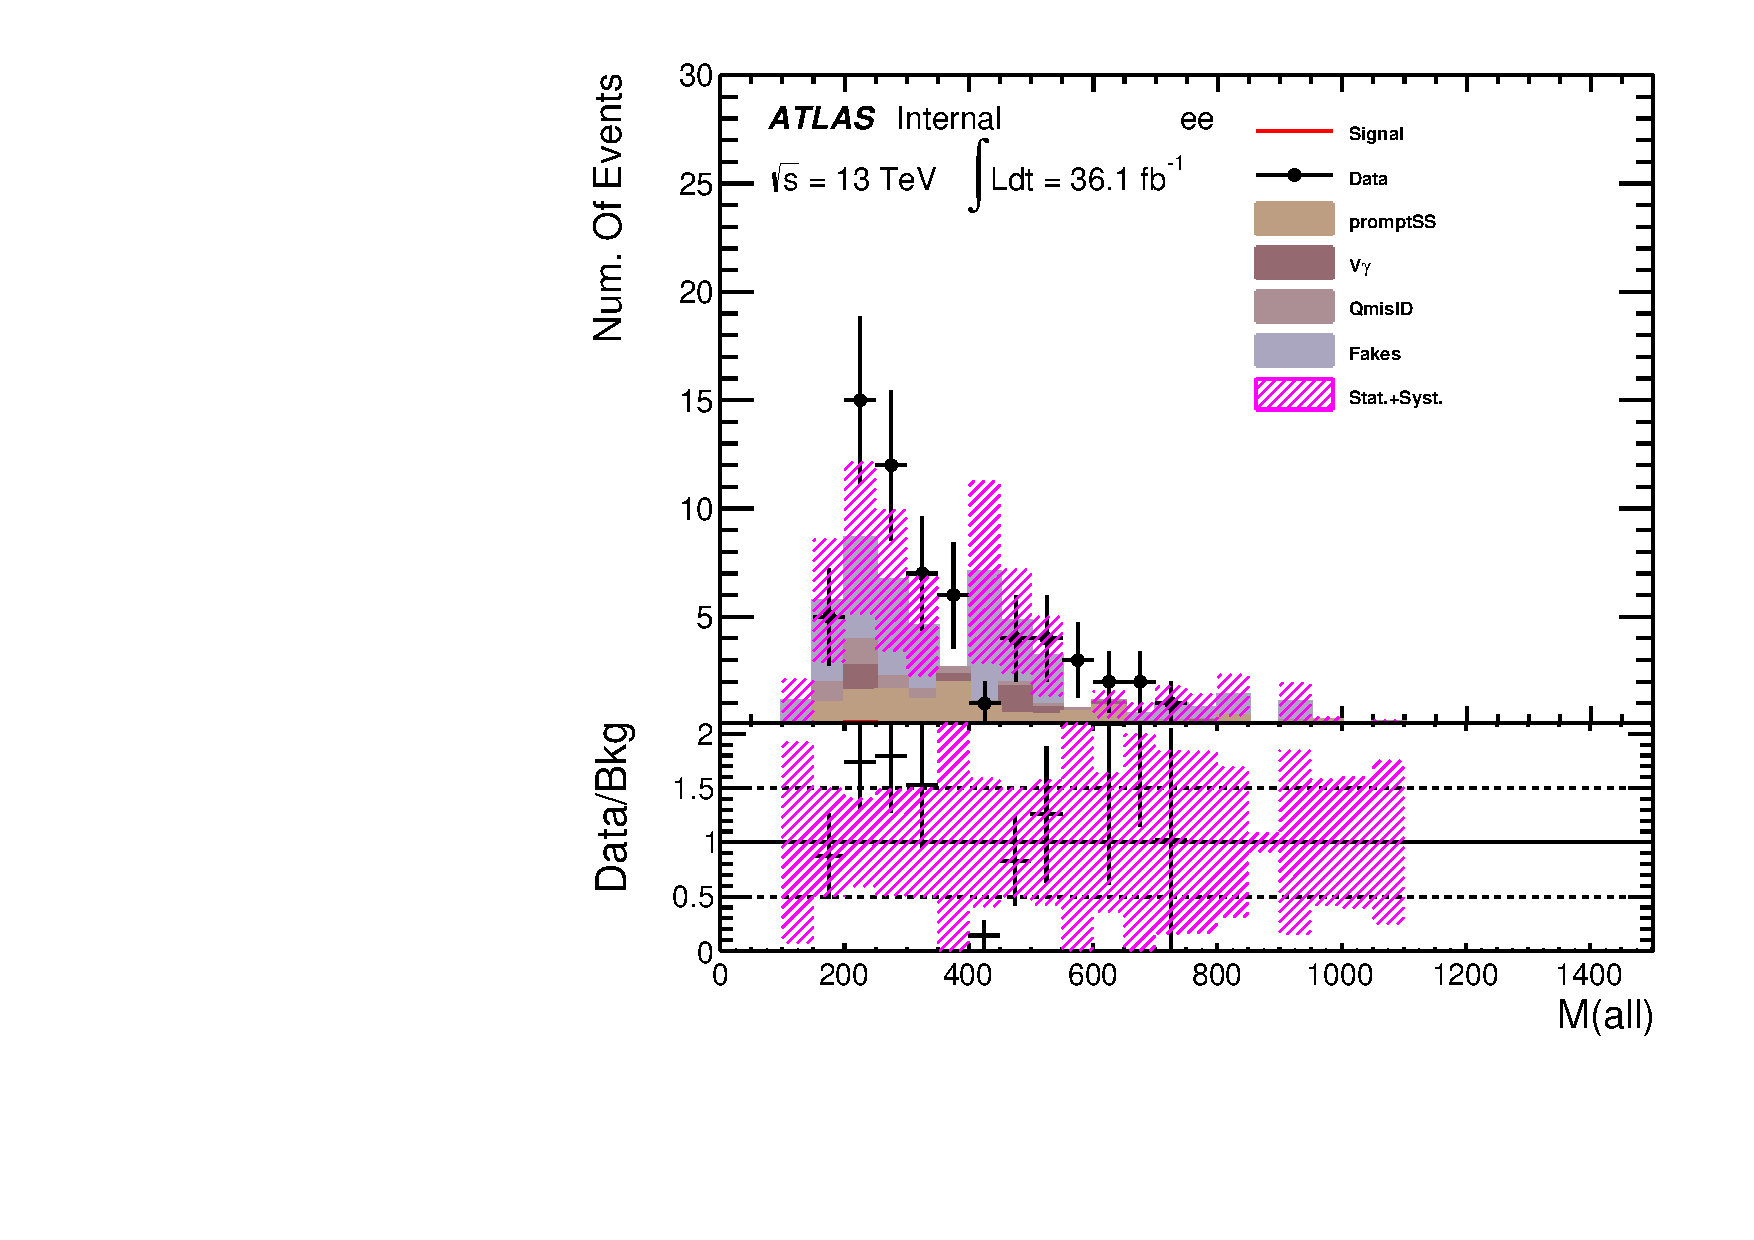
\includegraphics[width=0.9\textwidth,angle=-90]{fig/SigOpt/mH260_m_all_ee.pdf}
 \end{minipage}
 \begin{minipage}[t]{0.33\linewidth}
 \centering
 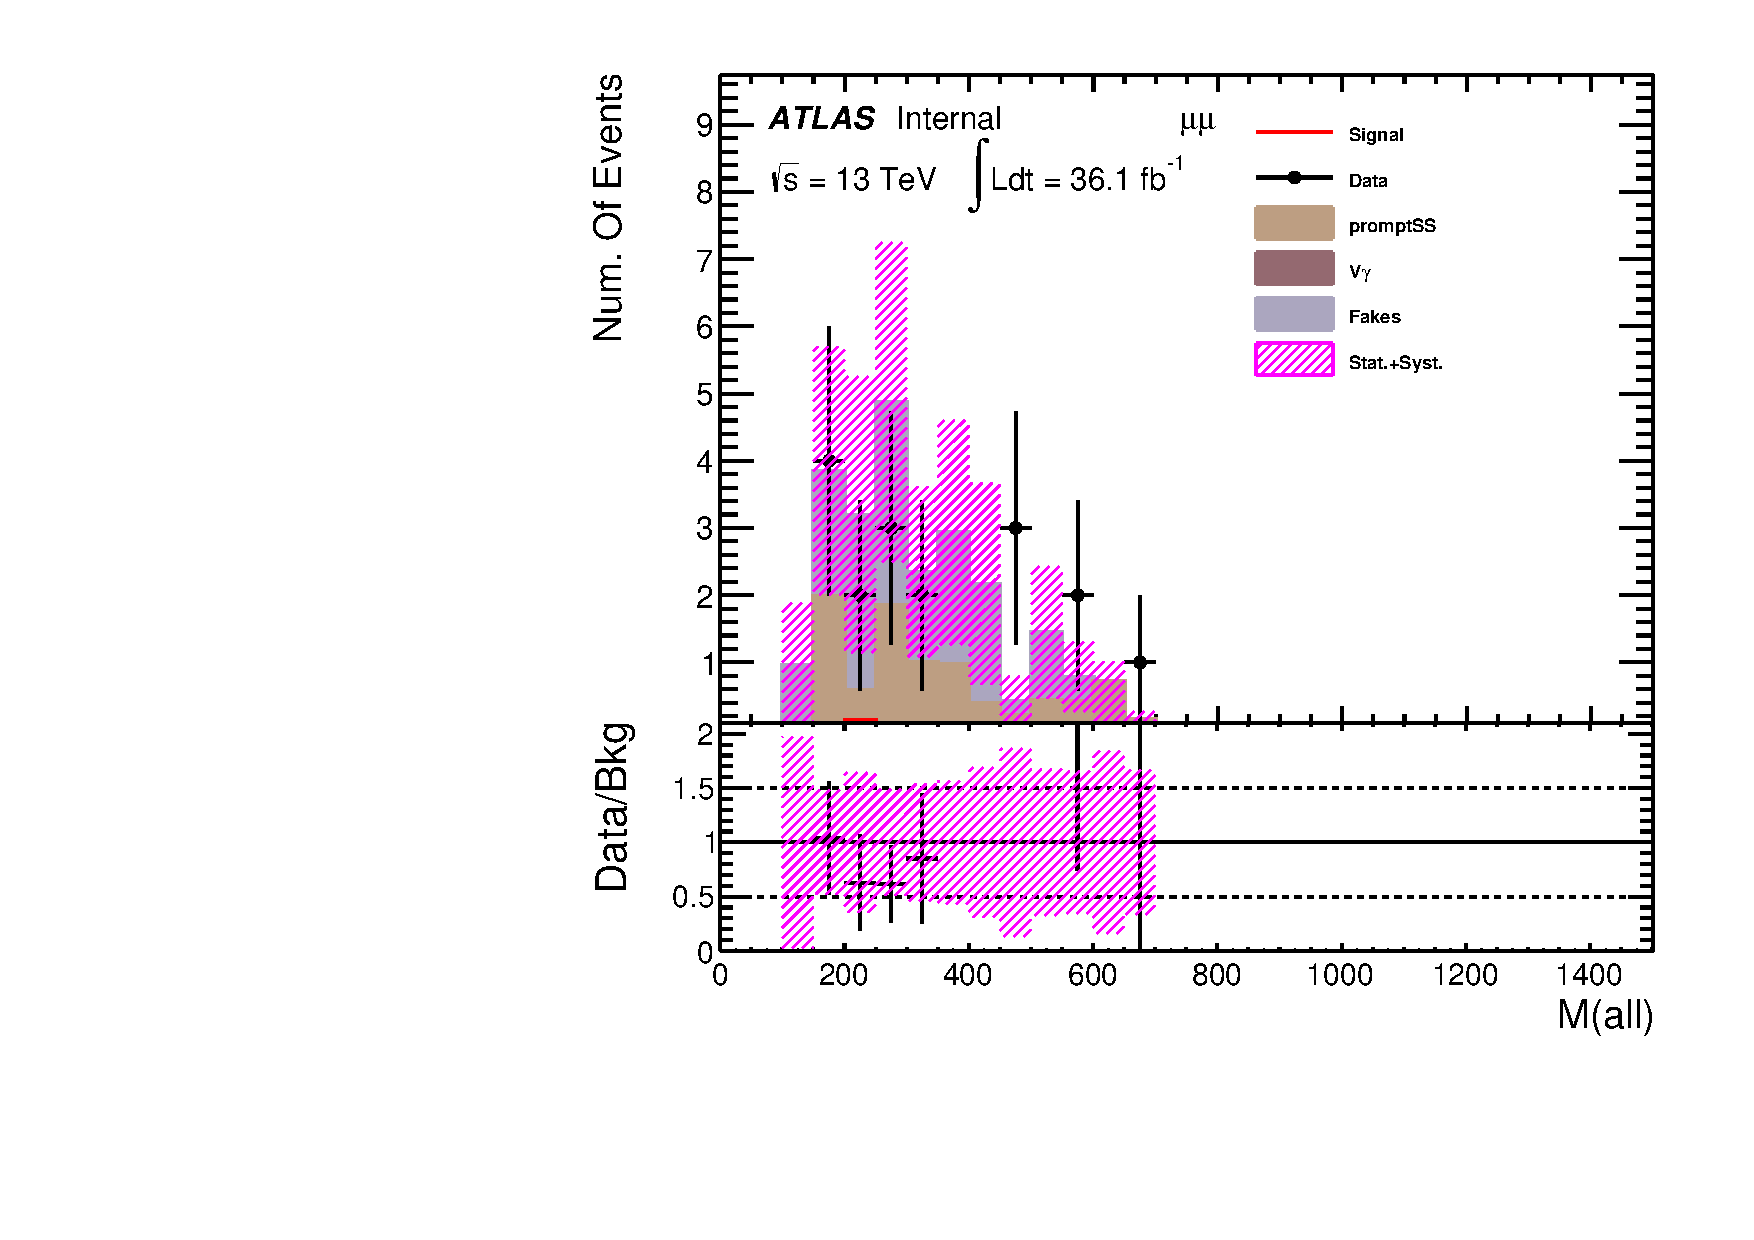
\includegraphics[width=0.9\textwidth,angle=-90]{fig/SigOpt/mH260_m_all_mumu.pdf}
 \end{minipage}
 \begin{minipage}[t]{0.33\linewidth}
 \centering
 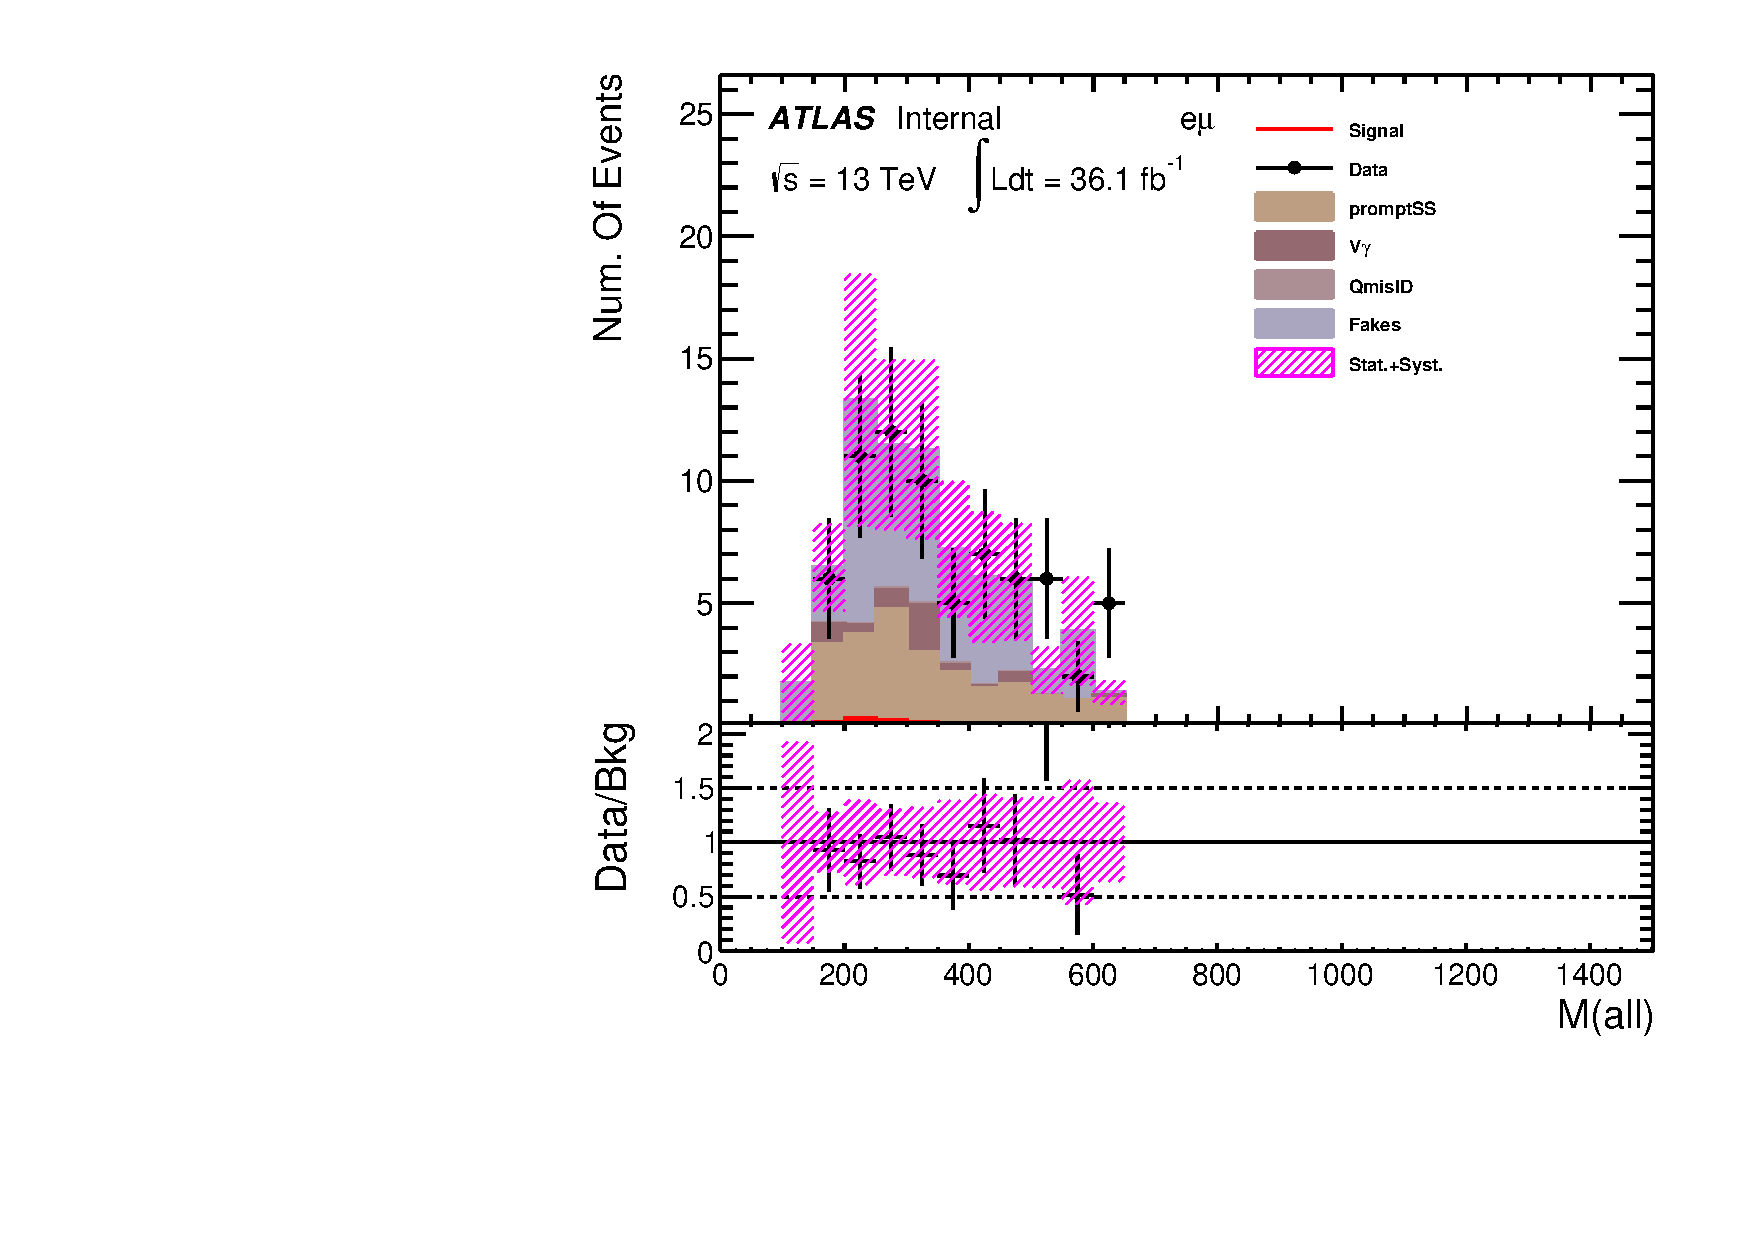
\includegraphics[width=0.9\textwidth,angle=-90]{fig/SigOpt/mH260_m_all_emu.pdf}
 \end{minipage}
 \caption{$m_X$=260 GeV质量点经过优化筛选之后$M(all)$分布。}
%\caption{The unblinded $M(all)$ distribution after all optimization selections, corresponding to resonance ($m_X$=260 GeV) search.}
\label{fig:SigOpt:mH260_m_l1jj.pdf}
\end{figure}

\begin{table}[h]
\begin{center}
\tiny\scalebox{0.8}{
\begin{tabular}{c|cccc|cc|c}
\hline
\hline
                          &promptSS  &$V+\gamma$  &QmisID  &Fakes  &Total bkg  &Observed  &signal  \\
\hline
$\Delta R_{min}(l_{2},j)$ &102.50$\pm$4.47(stat.)$\pm$30.75(syst.)  &33.03$\pm$5.51(stat.)$\pm$16.52(syst.)  &35.61$\pm$0.33(stat.)$\pm$11.75(syst.)  &128.89$\pm$8.34(stat.)$\pm$81.32(syst.)  &300.04$\pm$10.96(stat.)$\mp$36.83(syst1.)$\pm$81.32(syst2.)  &343  &0.80$\pm$0.03\\
\hline
$\Delta R_{min}(l_{1},j)$ &49.48$\pm$3.15(stat.)$\pm$14.84(syst.)  &22.72$\pm$5.05(stat.)$\pm$11.36(syst.)  &22.09$\pm$0.21(stat.)$\pm$7.29(syst.)  &92.54$\pm$7.07(stat.)$\pm$58.38(syst.)  &186.83$\pm$9.25(stat.)$\mp$20.06(syst1.)$\pm$58.38(syst2.)  &194  &0.74$\pm$0.03\\
\hline
$M(\ell\ell)$ &18.49$\pm$1.92(stat.)$\pm$5.55(syst.)  &5.31$\pm$2.21(stat.)$\pm$2.65(syst.)  &7.27$\pm$0.08(stat.)$\pm$2.40(syst.)  &36.86$\pm$4.46(stat.)$\pm$23.25(syst.)  &67.93$\pm$5.34(stat.)$\mp$6.60(syst1.)$\pm$23.25(syst2.)  &90  &0.61$\pm$0.03\\
\hline
$M(l_{1}jj)$ &18.15$\pm$1.91(stat.)$\pm$5.44(syst.)  &5.31$\pm$2.21(stat.)$\pm$2.65(syst.)  &7.22$\pm$0.08(stat.)$\pm$2.38(syst.)  &36.34$\pm$4.43(stat.)$\pm$22.93(syst.)  &67.02$\pm$5.31(stat.)$\mp$6.51(syst1.)$\pm$22.93(syst2.)  &89  &0.61$\pm$0.03\\
\hline
\hline
\end{tabular}}
\end{center}

\caption{$m_X$=300~GeV $ee$类别的优化结果。}
%\caption{The unblinded results of $m_X$=300~GeV search in $ee$ channel. }
\label{cutflow_ee_mX300}
\end{table}

\begin{table}[h]
\begin{center}
\tiny\scalebox{0.65}{
\begin{tabular}{c|cccc|cc|c}
\hline
\hline
                          &promptSS  &$V+\gamma$  &QmisID  &Fakes  &Total bkg  &Observed  &signal  \\
\hline
$\Delta R_{min}(l_{2},j)$ &169.68$\pm$6.15(stat.)$\pm$50.90(syst.)  &0.01$\pm$0.01(stat.)$\pm$0.00(syst.)  &0.00$\pm$0.00(stat.)$\pm$0.00(syst.)  &142.15$\pm$8.46(stat.)$\pm$91.75(syst.)  &311.83$\pm$10.46(stat.)$\mp$50.90(syst1.)$\pm$91.75(syst2.)  &245  &1.80$\pm$0.06\\
\hline
$\Delta R_{min}(l_{1},j)$ &97.25$\pm$4.96(stat.)$\pm$29.17(syst.)  &0.01$\pm$0.01(stat.)$\pm$0.00(syst.)  &0.00$\pm$0.00(stat.)$\pm$0.00(syst.)  &120.11$\pm$7.77(stat.)$\pm$77.53(syst.)  &217.36$\pm$9.22(stat.)$\mp$29.17(syst1.)$\pm$77.53(syst2.)  &141  &1.66$\pm$0.06\\
\hline
$M(\ell\ell)$ &50.83$\pm$3.33(stat.)$\pm$15.25(syst.)  &0.00$\pm$0.00(stat.)$\pm$0.00(syst.)  &0.00$\pm$0.00(stat.)$\pm$0.00(syst.)  &78.24$\pm$6.28(stat.)$\pm$50.51(syst.)  &129.07$\pm$7.11(stat.)$\mp$15.25(syst1.)$\pm$50.51(syst2.)  &79  &1.47$\pm$0.05\\
\hline
$M(l_{1}jj)$ &47.98$\pm$3.29(stat.)$\pm$14.39(syst.)  &0.00$\pm$0.00(stat.)$\pm$0.00(syst.)  &0.00$\pm$0.00(stat.)$\pm$0.00(syst.)  &77.49$\pm$6.25(stat.)$\pm$50.02(syst.)  &125.47$\pm$7.06(stat.)$\mp$14.39(syst1.)$\pm$50.02(syst2.)  &74  &1.46$\pm$0.05\\
\hline
\hline
\end{tabular}}
\end{center}

\caption{$m_X$=300~GeV $\mu\mu$类别的优化结果。}
%\caption{The unblinded results of $m_X$=300~GeV search in $\mu\mu$ channel. }
\label{cutflow_mumu_mX300}
\end{table}

\begin{table}[h]
\begin{center}
\tiny\scalebox{0.8}{
\begin{tabular}{c|cccc|cc|c}
\hline
\hline
                          &promptSS  &$V+\gamma$  &QmisID  &Fakes  &Total bkg  &Observed  &signal  \\
\hline
$\Delta R_{min}(l_{2},j)$ &285.01$\pm$7.13(stat.)$\pm$85.50(syst.)  &36.28$\pm$5.39(stat.)$\pm$18.14(syst.)  &9.46$\pm$0.16(stat.)$\pm$3.12(syst.)  &170.21$\pm$9.47(stat.)$\pm$79.34(syst.)  &500.96$\pm$13.02(stat.)$\mp$87.46(syst1.)$\pm$79.34(syst2.)  &596  &2.64$\pm$0.07\\
\hline
$\Delta R_{min}(l_{1},j)$ &182.33$\pm$5.88(stat.)$\pm$54.70(syst.)  &26.12$\pm$4.79(stat.)$\pm$13.06(syst.)  &3.99$\pm$0.07(stat.)$\pm$1.32(syst.)  &139.61$\pm$8.57(stat.)$\pm$64.37(syst.)  &352.05$\pm$11.44(stat.)$\mp$56.25(syst1.)$\pm$64.37(syst2.)  &397  &2.57$\pm$0.07\\
\hline
$M(\ell\ell)$ &68.67$\pm$3.59(stat.)$\pm$20.60(syst.)  &10.73$\pm$2.76(stat.)$\pm$5.36(syst.)  &1.41$\pm$0.03(stat.)$\pm$0.47(syst.)  &66.72$\pm$5.92(stat.)$\pm$30.48(syst.)  &147.52$\pm$7.45(stat.)$\mp$21.29(syst1.)$\pm$30.48(syst2.)  &163  &2.05$\pm$0.06\\
\hline
$M(l_{1}jj)$ &59.41$\pm$3.38(stat.)$\pm$17.82(syst.)  &8.94$\pm$2.50(stat.)$\pm$4.47(syst.)  &1.24$\pm$0.03(stat.)$\pm$0.41(syst.)  &62.74$\pm$5.74(stat.)$\pm$28.94(syst.)  &132.33$\pm$7.12(stat.)$\mp$18.38(syst1.)$\pm$28.94(syst2.)  &144  &1.99$\pm$0.06\\
\hline
\hline
\end{tabular}}
\end{center}

\caption{$m_X$=300~GeV $e\mu$类别的优化结果。}
%\caption{The unblinded results of $m_X$=300~GeV search in $e\mu$ channel. }
\label{cutflow_emu_mX300}
\end{table}

\begin{figure}[h]
\begin{minipage}[t]{0.33\linewidth}
 \centering
 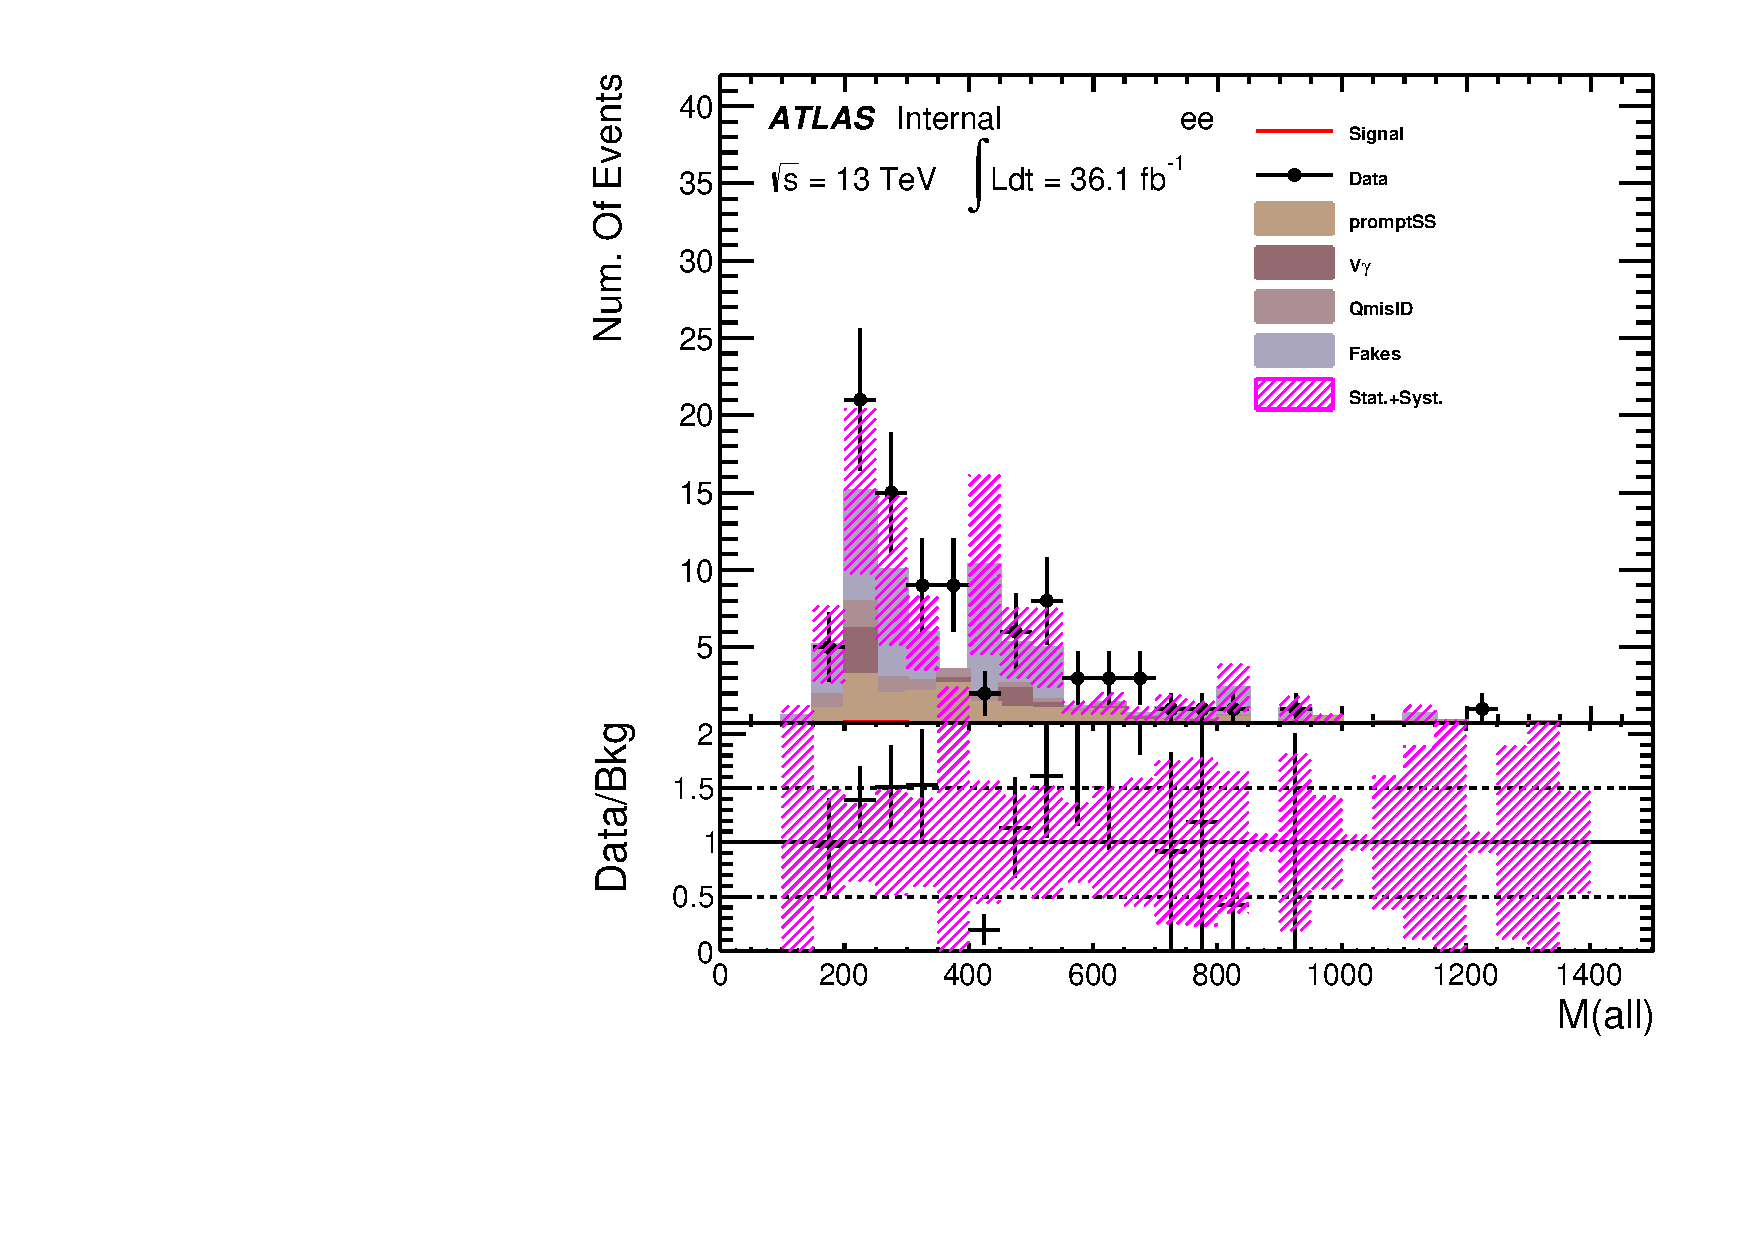
\includegraphics[width=0.9\textwidth,angle=-90]{fig/SigOpt/mH300_m_all_ee.pdf}
 \end{minipage}
 \begin{minipage}[t]{0.33\linewidth}
 \centering
 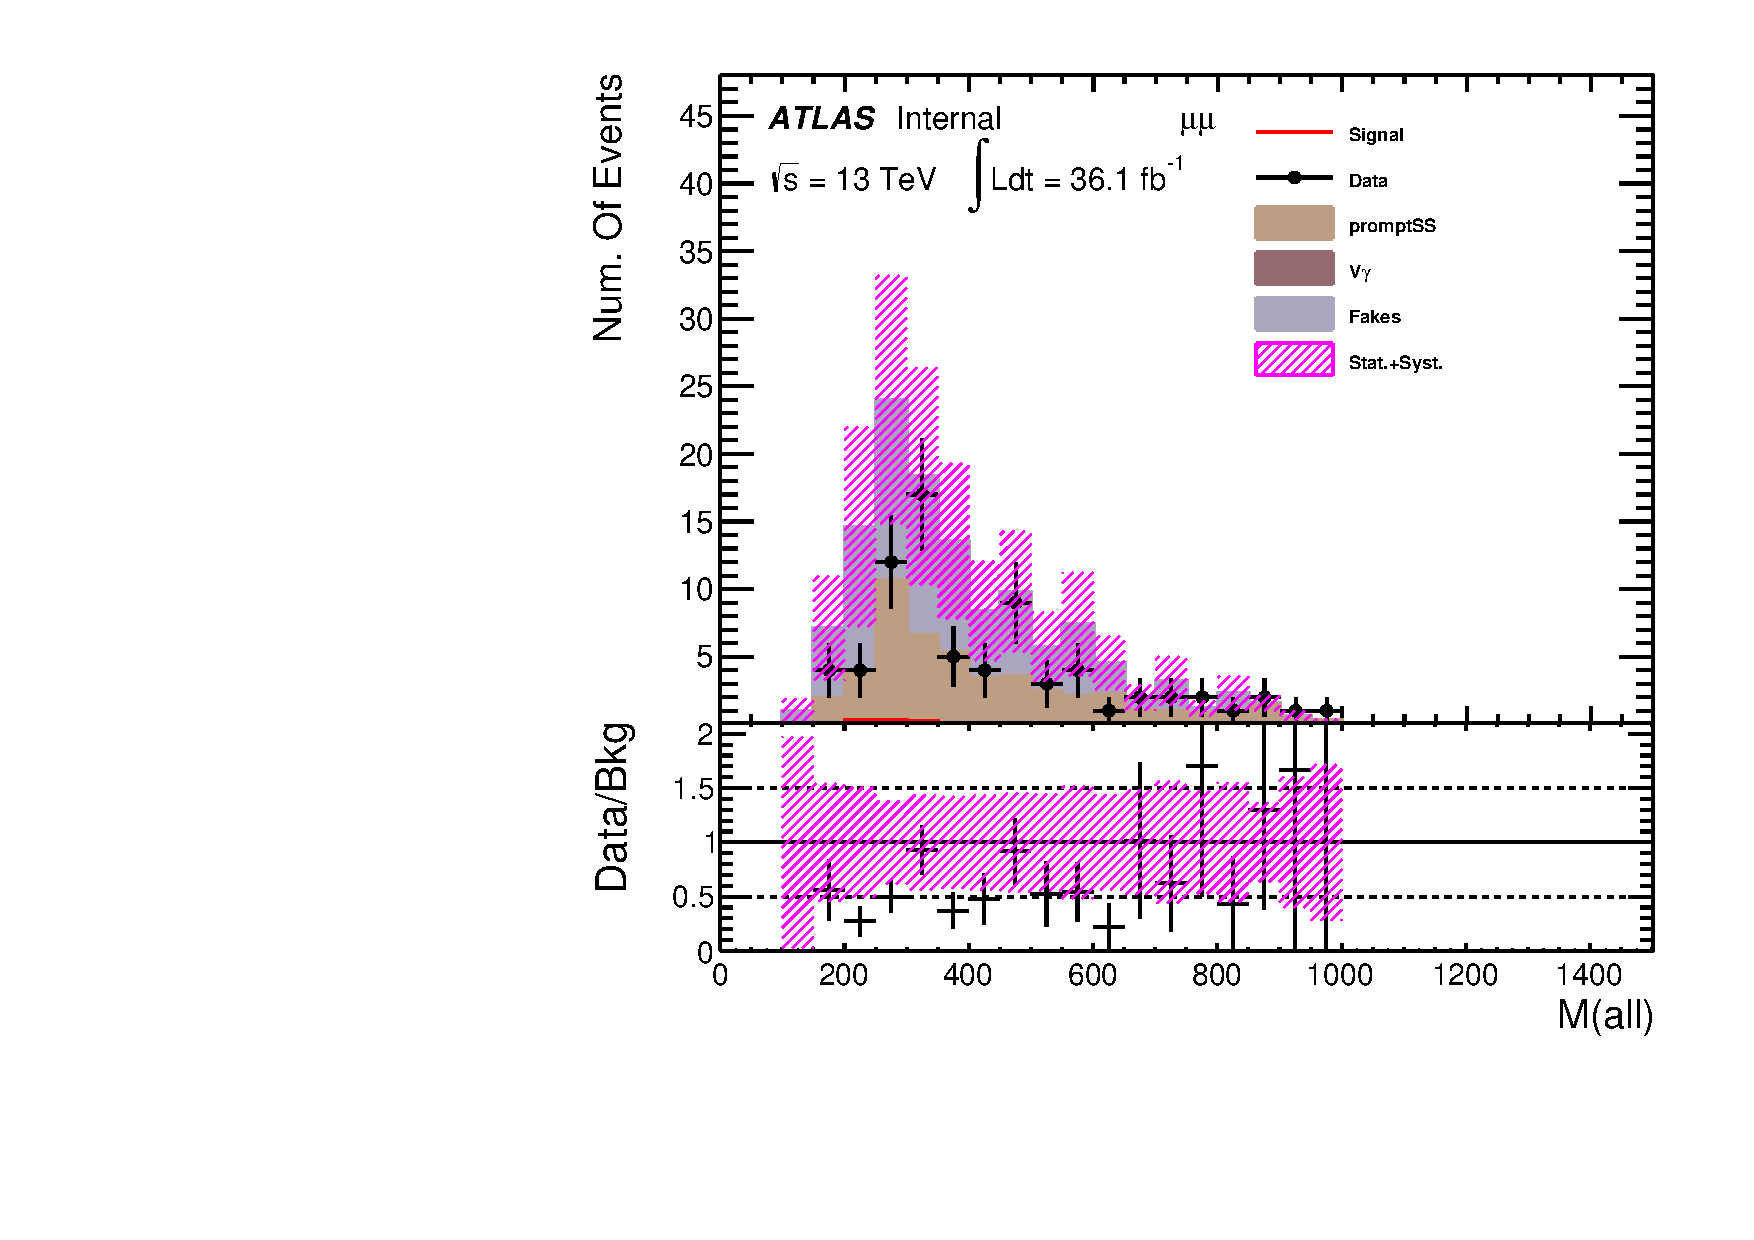
\includegraphics[width=0.9\textwidth,angle=-90]{fig/SigOpt/mH300_m_all_mumu.pdf}
 \end{minipage}
 \begin{minipage}[t]{0.33\linewidth}
 \centering
 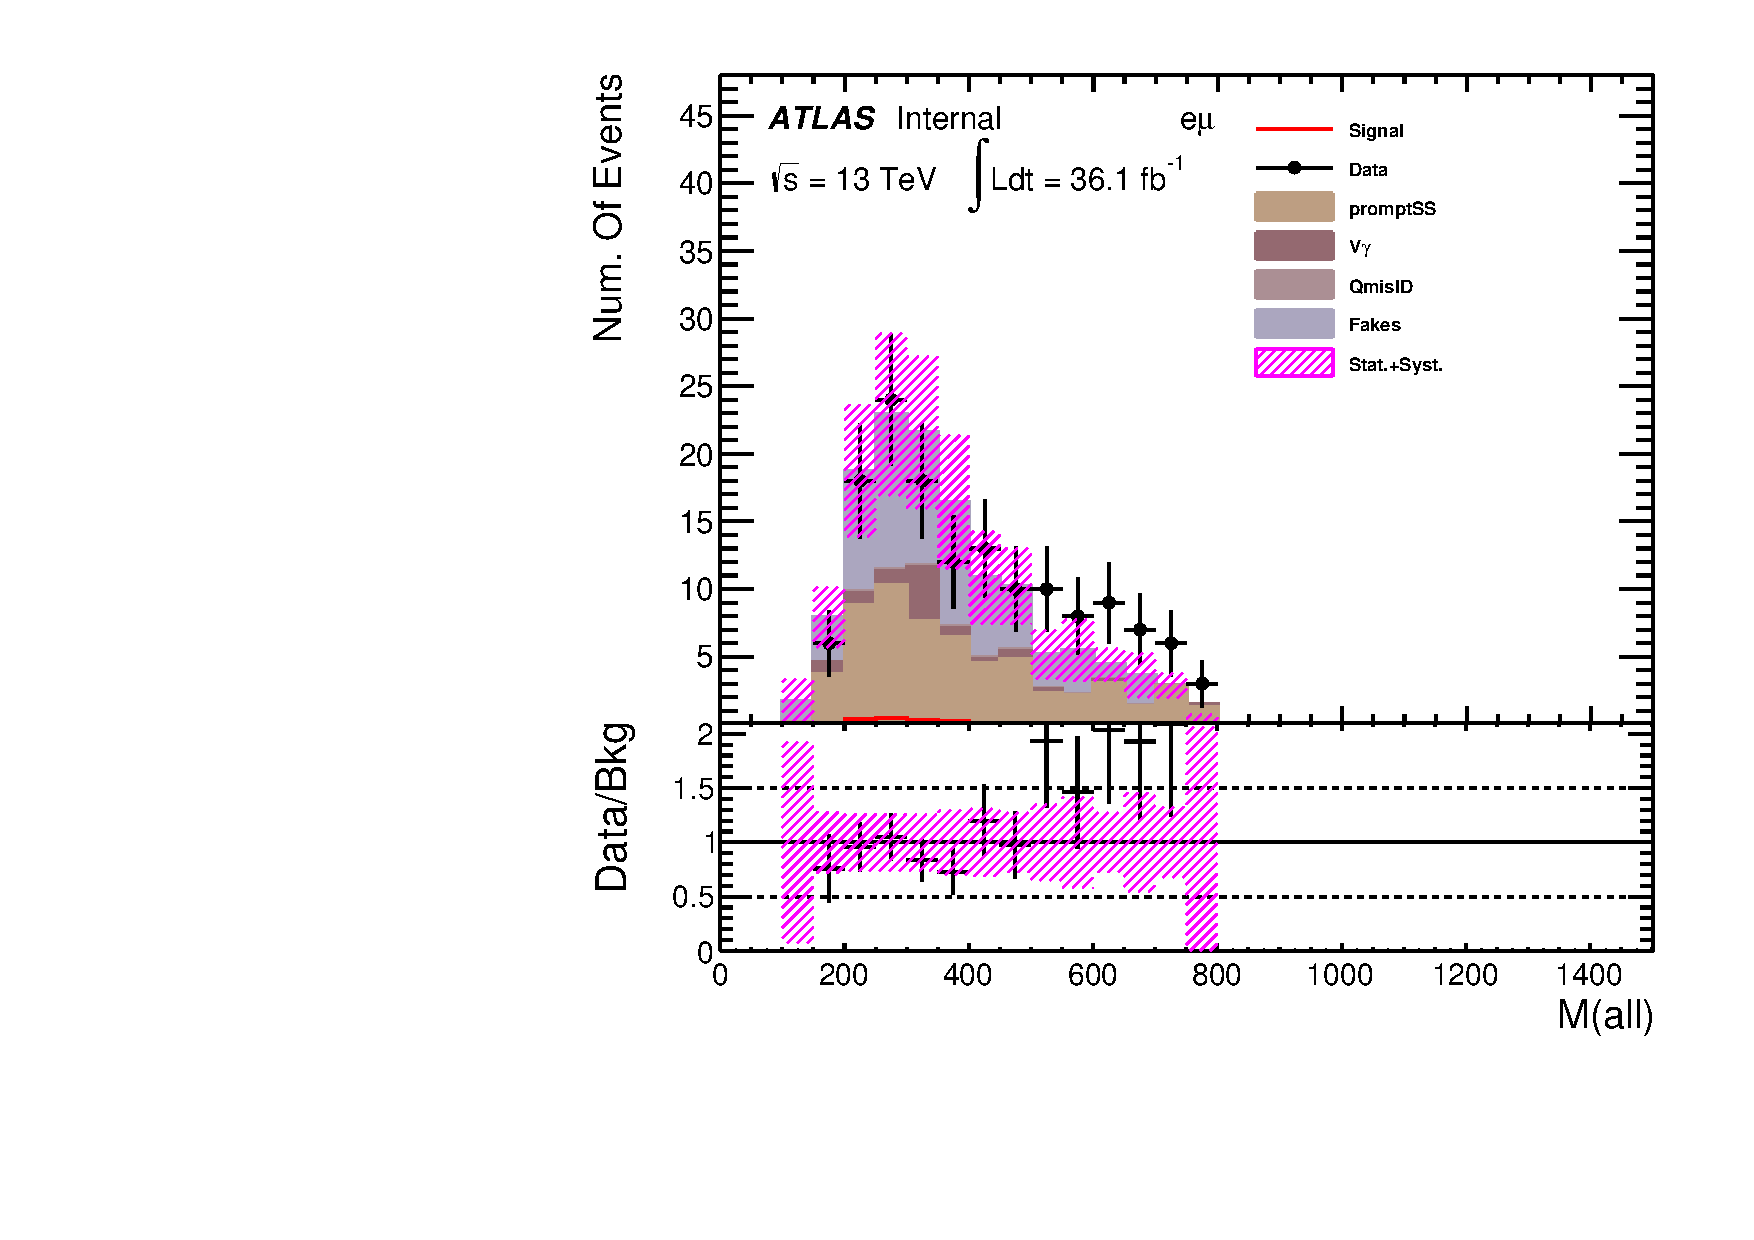
\includegraphics[width=0.9\textwidth,angle=-90]{fig/SigOpt/mH300_m_all_emu.pdf}
 \end{minipage}
 \caption{$m_X$=300 GeV质量点经过优化筛选之后$M(all)$分布。}
%\caption{The unblinded $M(all)$ distribution after all optimization selections, corresponding to resonance ($m_X$=300 GeV) search.}
\label{fig:SigOpt:mH300_m_l1jj.pdf}
\end{figure}

\begin{table}[h]
\begin{center}
\tiny\scalebox{0.8}{
\begin{tabular}{c|cccc|cc|c}
\hline
\hline
                           &promptSS  &$V+\gamma$  &QmisID  &Fakes  &Total bkg  &Observed  &signal  \\  
\hline
$\Delta R_{min}(l_{2},j)$ &52.12$\pm$3.04(stat.)$\pm$15.64(syst.)  &17.85$\pm$4.08(stat.)$\pm$8.93(syst.)  &17.54$\pm$0.26(stat.)$\pm$5.79(syst.)  &69.22$\pm$6.15(stat.)$\pm$47.89(syst.)  &156.73$\pm$7.99(stat.)$\mp$18.91(syst1.)$\pm$47.89(syst2.)  &182  &3.33$\pm$0.08\\
\hline
$\Delta R_{min}(l_{1},j)$ &20.98$\pm$1.96(stat.)$\pm$6.29(syst.)  &3.51$\pm$1.10(stat.)$\pm$1.76(syst.)  &6.68$\pm$0.15(stat.)$\pm$2.20(syst.)  &27.96$\pm$3.91(stat.)$\pm$19.35(syst.)  &59.14$\pm$4.52(stat.)$\mp$6.90(syst1.)$\pm$19.35(syst2.)  &75  &2.34$\pm$0.07\\
\hline
$M(\ell\ell)$ &16.15$\pm$1.83(stat.)$\pm$4.85(syst.)  &1.25$\pm$0.42(stat.)$\pm$0.63(syst.)  &4.50$\pm$0.12(stat.)$\pm$1.49(syst.)  &21.82$\pm$3.46(stat.)$\pm$15.09(syst.)  &43.73$\pm$3.93(stat.)$\mp$5.11(syst1.)$\pm$15.09(syst2.)  &59  &2.27$\pm$0.07\\
\hline
$M(l_{1}jj)$ &11.56$\pm$1.25(stat.)$\pm$3.47(syst.)  &0.83$\pm$0.34(stat.)$\pm$0.41(syst.)  &3.46$\pm$0.10(stat.)$\pm$1.14(syst.)  &19.09$\pm$3.23(stat.)$\pm$13.21(syst.)  &34.94$\pm$3.48(stat.)$\mp$3.67(syst1.)$\pm$13.21(syst2.)  &46  &2.16$\pm$0.07\\
\hline
\hline
\end{tabular}}
\end{center}

\caption{$m_X$=400~GeV $ee$类别的优化结果。}
%\caption{The unblinded results of $m_X$=400~GeV search in $ee$ channel. }
\label{cutflow_ee_mX400}
\end{table}

\begin{table}[h]
\begin{center}
\tiny\scalebox{0.65}{
\begin{tabular}{c|cccc|cc|c}
\hline
\hline
                           &promptSS  &$V+\gamma$  &QmisID  &Fakes  &Total bkg  &Observed  &signal  \\  
\hline
$\Delta R_{min}(l_{2},j)$ &59.36$\pm$3.01(stat.)$\pm$17.81(syst.)  &0.01$\pm$0.01(stat.)$\pm$0.00(syst.)  &0.00$\pm$0.00(stat.)$\pm$0.00(syst.)  &51.25$\pm$4.83(stat.)$\pm$36.79(syst.)  &110.61$\pm$5.69(stat.)$\mp$17.81(syst1.)$\pm$36.79(syst2.)  &99  &1.72$\pm$0.06\\
\hline
$\Delta R_{min}(l_{1},j)$ &25.36$\pm$1.92(stat.)$\pm$7.61(syst.)  &0.00$\pm$0.00(stat.)$\pm$0.00(syst.)  &0.00$\pm$0.00(stat.)$\pm$0.00(syst.)  &18.80$\pm$2.92(stat.)$\pm$13.50(syst.)  &44.17$\pm$3.50(stat.)$\mp$7.61(syst1.)$\pm$13.50(syst2.)  &37  &1.38$\pm$0.05\\
\hline
$M(\ell\ell)$ &18.50$\pm$1.72(stat.)$\pm$5.55(syst.)  &0.00$\pm$0.00(stat.)$\pm$0.00(syst.)  &0.00$\pm$0.00(stat.)$\pm$0.00(syst.)  &17.02$\pm$2.78(stat.)$\pm$12.22(syst.)  &35.51$\pm$3.27(stat.)$\mp$5.55(syst1.)$\pm$12.22(syst2.)  &26  &1.34$\pm$0.05\\
\hline
$M(l_{1}jj)$ &13.82$\pm$1.38(stat.)$\pm$4.15(syst.)  &0.00$\pm$0.00(stat.)$\pm$0.00(syst.)  &0.00$\pm$0.00(stat.)$\pm$0.00(syst.)  &14.09$\pm$2.53(stat.)$\pm$10.11(syst.)  &27.91$\pm$2.88(stat.)$\mp$4.15(syst1.)$\pm$10.11(syst2.)  &19  &1.30$\pm$0.05\\
\hline
\hline
\end{tabular}}
\end{center}

\caption{$m_X$=400~GeV $\mu\mu$类别的优化结果。}
%\caption{The unblinded results of $m_X$=400~GeV search in $\mu\mu$ channel. }
\label{cutflow_mumu_mX400}
\end{table}

\begin{table}[h]
\begin{center}
\tiny\scalebox{0.65}{
\begin{tabular}{c|cccc|cc|c}
\hline
\hline
                           &promptSS  &$V+\gamma$  &QmisID  &Fakes  &Total bkg  &Observed  &signal  \\  
\hline
$\Delta R_{min}(l_{2},j)$ &145.72$\pm$5.10(stat.)$\pm$43.72(syst.)  &23.17$\pm$4.97(stat.)$\pm$11.59(syst.)  &5.06$\pm$0.13(stat.)$\pm$1.67(syst.)  &72.77$\pm$6.07(stat.)$\pm$36.36(syst.)  &246.72$\pm$9.35(stat.)$\mp$45.26(syst1.)$\pm$36.36(syst2.)  &283  &3.33$\pm$0.08 \\
\hline
$\Delta R_{min}(l_{1},j)$ &46.01$\pm$2.73(stat.)$\pm$13.80(syst.)  &7.96$\pm$3.23(stat.)$\pm$3.98(syst.)  &1.69$\pm$0.07(stat.)$\pm$0.56(syst.)  &27.03$\pm$3.75(stat.)$\pm$14.31(syst.)  &82.70$\pm$5.65(stat.)$\mp$14.38(syst1.)$\pm$14.31(syst2.)  &93  &2.34$\pm$0.07 \\
\hline
$M(\ell\ell)$ &33.90$\pm$2.37(stat.)$\pm$10.17(syst.)  &6.54$\pm$3.20(stat.)$\pm$3.27(syst.)  &0.86$\pm$0.04(stat.)$\pm$0.28(syst.)  &20.86$\pm$3.29(stat.)$\pm$11.11(syst.)  &62.16$\pm$5.17(stat.)$\mp$10.69(syst1.)$\pm$11.11(syst2.)  &69  &2.27$\pm$0.07\\
\hline
$M(l_{1}jj)$ &24.13$\pm$1.97(stat.)$\pm$7.24(syst.)  &2.47$\pm$1.25(stat.)$\pm$1.23(syst.)  &0.60$\pm$0.03(stat.)$\pm$0.20(syst.)  &17.82$\pm$3.06(stat.)$\pm$9.80(syst.)  &45.02$\pm$3.84(stat.)$\mp$7.35(syst1.)$\pm$9.80(syst2.)  &57  &2.16$\pm$0.07\\
\hline
\hline
\end{tabular}}
\end{center}

\caption{$m_X$=400~GeV $e\mu$类别的优化结果。}
%\caption{The unblinded results of $m_X$=400~GeV search in $e\mu$ channel. }
\label{cutflow_emu_mX400}
\end{table}

\begin{figure}[h]
\begin{minipage}[t]{0.33\linewidth}
 \centering
 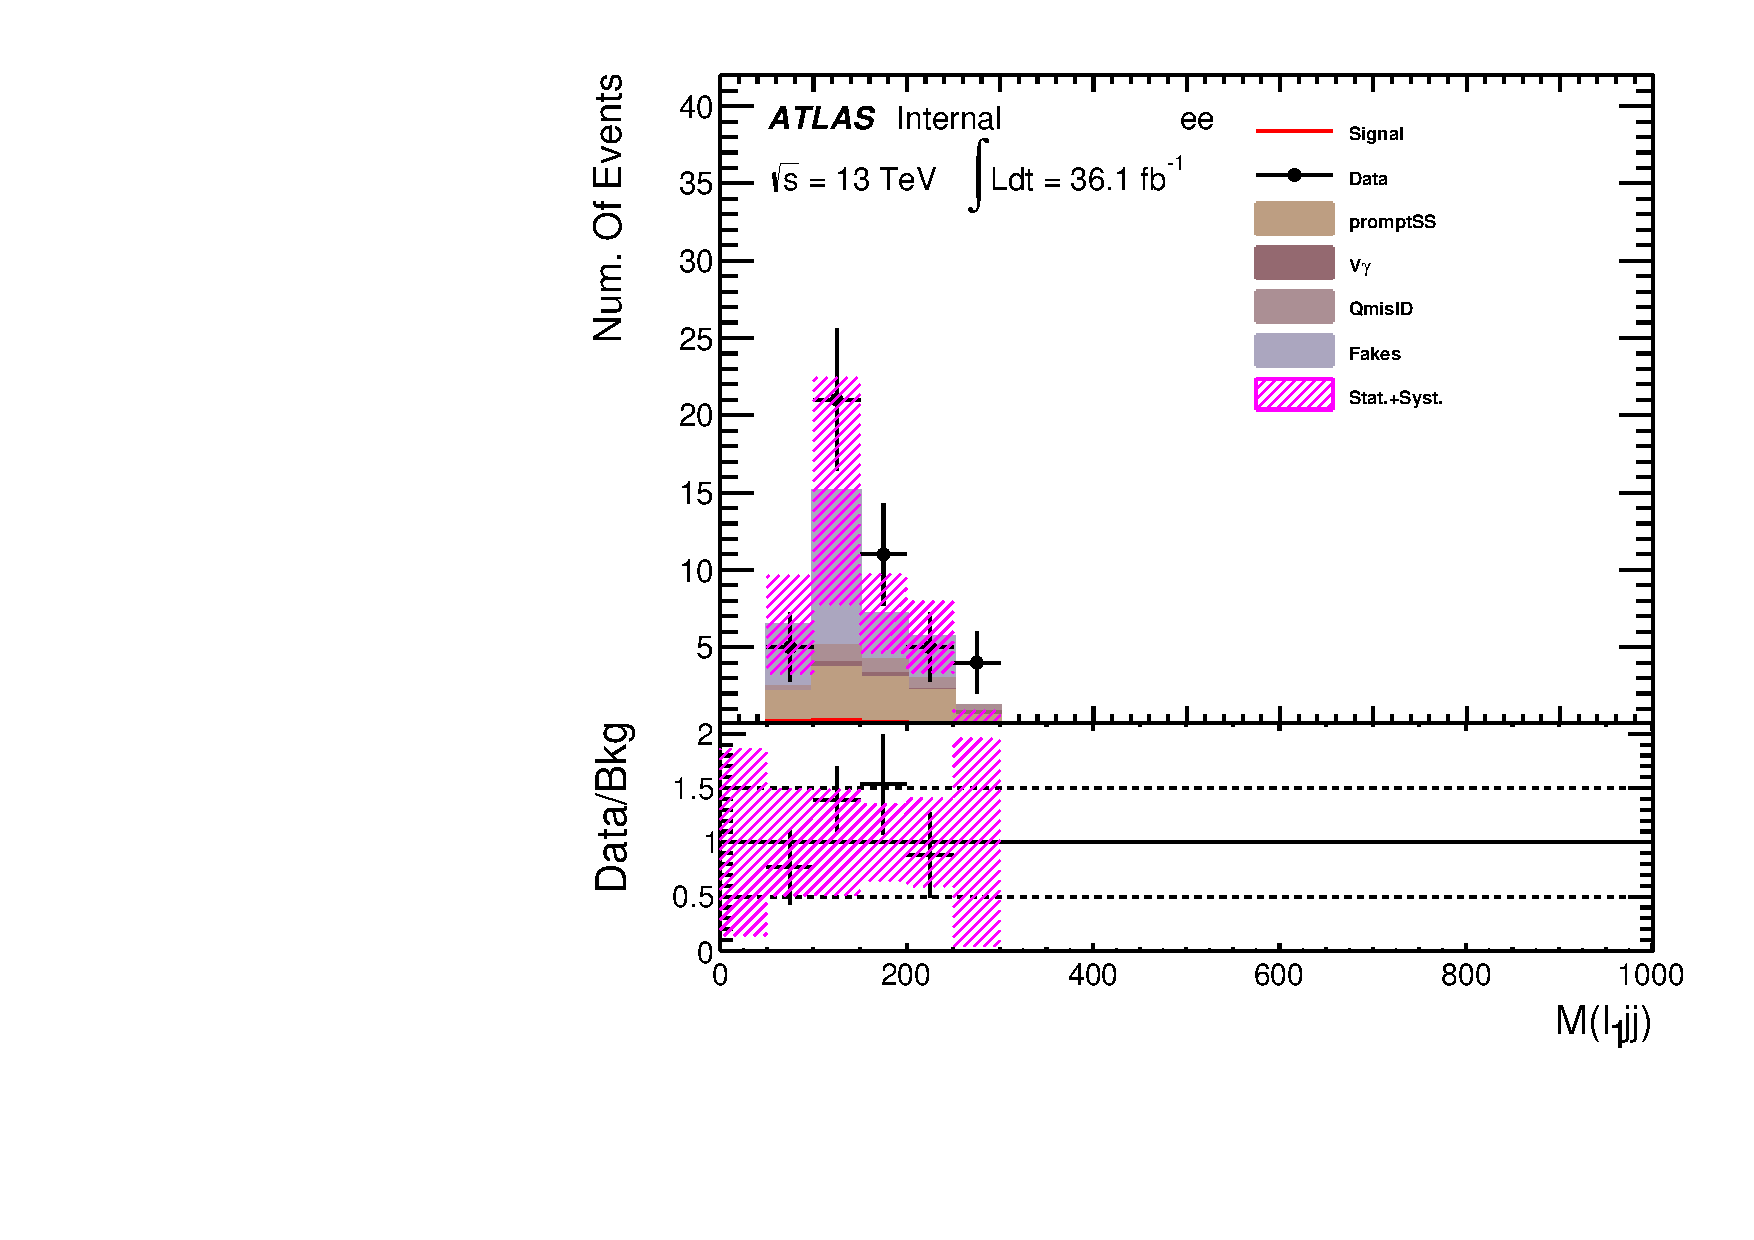
\includegraphics[width=0.9\textwidth,angle=-90]{fig/SigOpt/mH400_m_l1jj_ee.pdf}
 \end{minipage}
 \begin{minipage}[t]{0.33\linewidth}
 \centering
 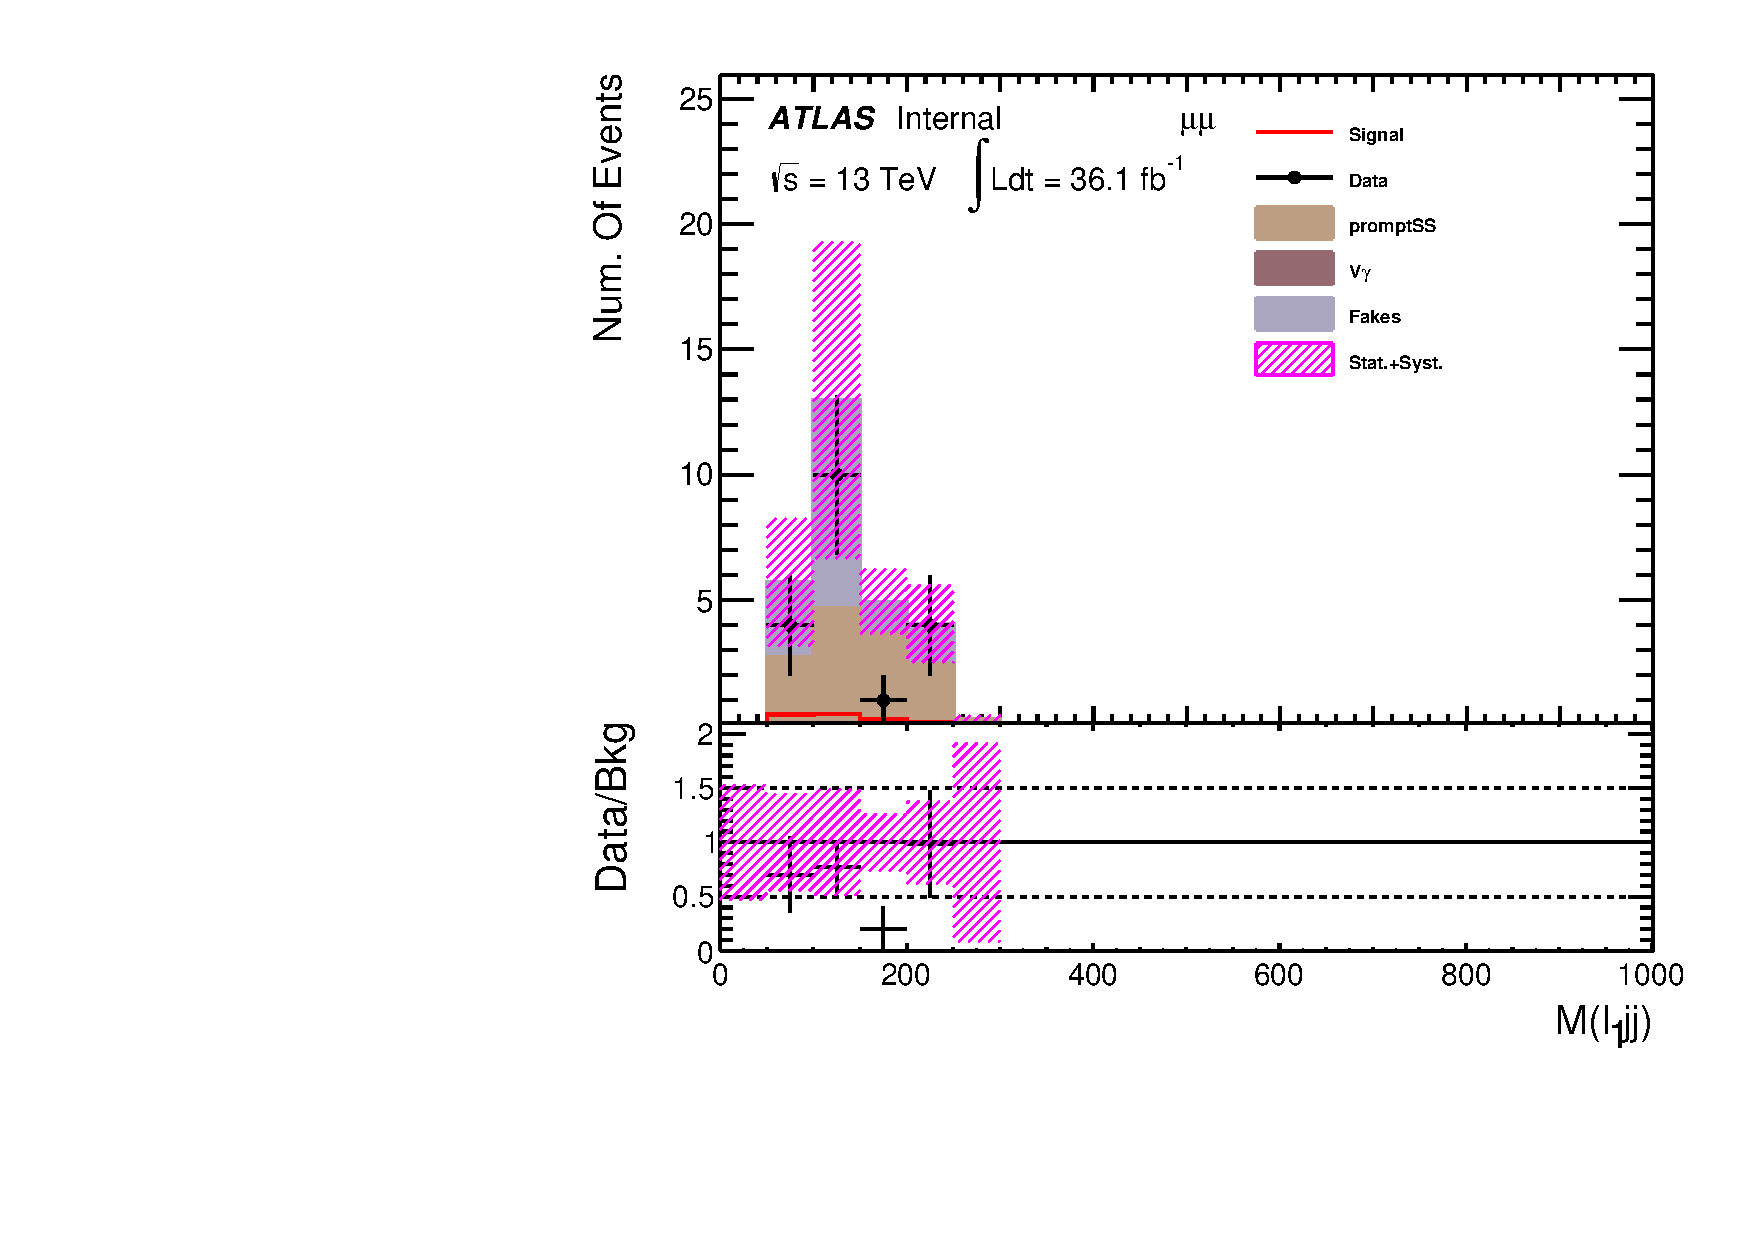
\includegraphics[width=0.9\textwidth,angle=-90]{fig/SigOpt/mH400_m_l1jj_mumu.pdf}
 \end{minipage}
 \begin{minipage}[t]{0.33\linewidth}
 \centering
 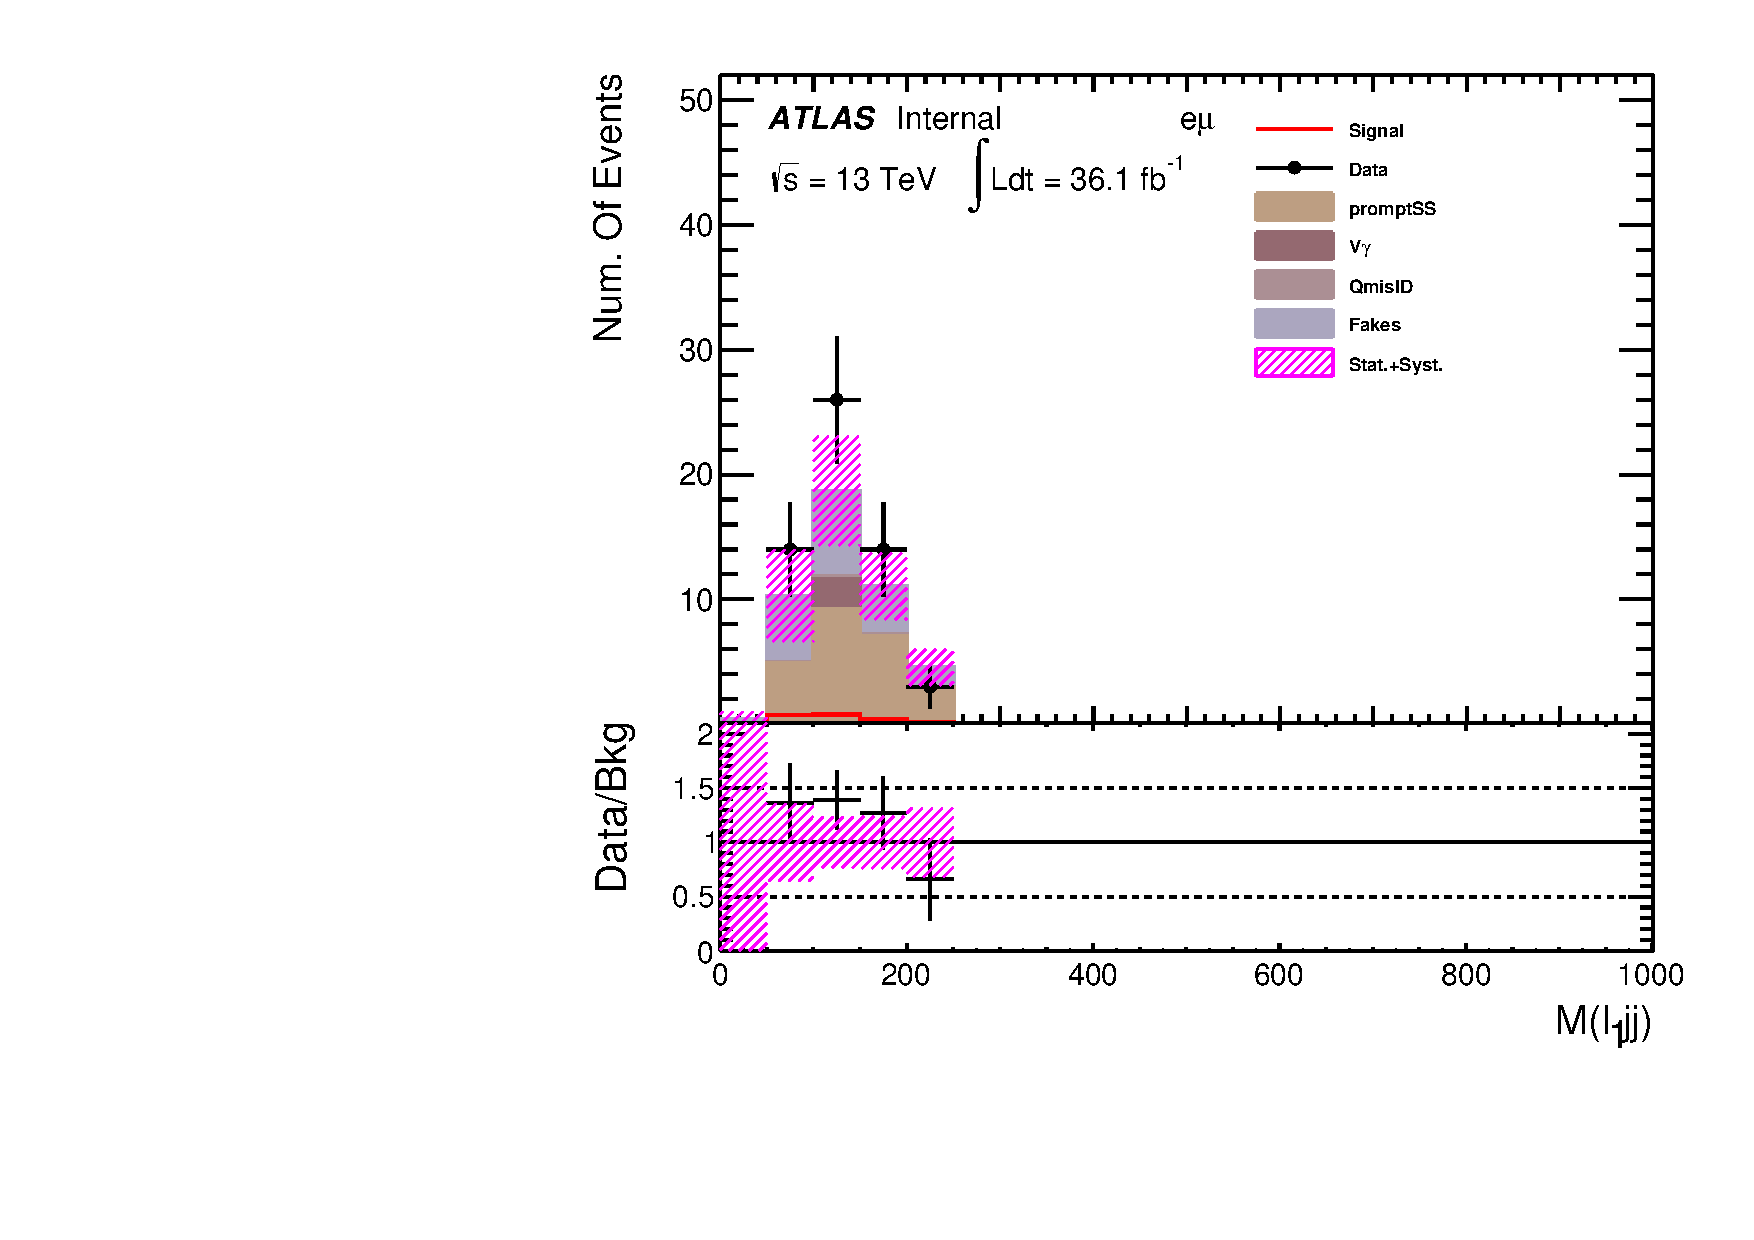
\includegraphics[width=0.9\textwidth,angle=-90]{fig/SigOpt/mH400_m_l1jj_emu.pdf}
 \end{minipage}
 \caption{$m_X$=400 GeV质量点经过优化筛选之后$M(\ell_{1}jj)$分布。}
%\caption{The unblinded $M(\ell_{1}jj)$ distribution after all optimization selections, corresponding to resonance ($m_X$=400 GeV) search.}
\label{fig:SigOpt:mH400_m_l1jj.pdf}
\end{figure}

\begin{table}[h]
\begin{center}
\tiny\scalebox{0.65}{
\begin{tabular}{c|cccc|cc|c}
\hline
\hline
                           &promptSS  &$V+\gamma$  &QmisID  &Fakes  &Total bkg  &Observed  &signal  \\  
\hline
$\Delta R_{min}(l_{2},j)$ &36.10$\pm$2.66(stat.)$\pm$10.83(syst.)  &12.21$\pm$3.77(stat.)$\pm$6.10(syst.)  &11.32$\pm$0.21(stat.)$\pm$3.73(syst.)  &49.72$\pm$5.22(stat.)$\pm$34.39(syst.)  &109.34$\pm$6.96(stat.)$\mp$12.98(syst1.)$\pm$34.39(syst2.)  &117  &1.40$\pm$0.05\\
\hline
$\Delta R_{min}(l_{1},j)$ &13.11$\pm$1.68(stat.)$\pm$3.93(syst.)  &1.89$\pm$0.95(stat.)$\pm$0.94(syst.)  &4.00$\pm$0.12(stat.)$\pm$1.32(syst.)  &17.81$\pm$3.12(stat.)$\pm$12.32(syst.)  &36.81$\pm$3.67(stat.)$\mp$4.26(syst1.)$\pm$12.32(syst2.)  &47  &1.13$\pm$0.04\\
\hline
$M(\ell\ell)$ &5.40$\pm$0.79(stat.)$\pm$1.62(syst.)  &0.36$\pm$0.19(stat.)$\pm$0.18(syst.)  &1.59$\pm$0.08(stat.)$\pm$0.53(syst.)  &6.65$\pm$1.91(stat.)$\pm$4.60(syst.)  &14.01$\pm$2.08(stat.)$\mp$1.71(syst1.)$\pm$4.60(syst2.)  &21  &0.90$\pm$0.04\\
\hline
$M(l_{1}jj)$ &3.92$\pm$0.70(stat.)$\pm$1.17(syst.)  &0.12$\pm$0.05(stat.)$\pm$0.06(syst.)  &1.24$\pm$0.07(stat.)$\pm$0.41(syst.)  &4.03$\pm$1.48(stat.)$\pm$2.79(syst.)  &9.31$\pm$1.64(stat.)$\mp$1.25(syst1.)$\pm$2.79(syst2.)  &14  &0.85$\pm$0.04\\
\hline
\hline
\end{tabular}}
\end{center}

\caption{$m_X$=500~GeV $ee$类别的优化结果。}
%\caption{The unblinded results of $m_X$=500~GeV search in $ee$ channel. }
\label{cutflow_ee_mX500}
\end{table}

\begin{table}[h]
\begin{center}
\tiny\scalebox{0.8}{
\begin{tabular}{c|cccc|cc|c}
\hline
\hline
                           &promptSS  &$V+\gamma$  &QmisID  &Fakes  &Total bkg  &Observed  &signal  \\  
\hline
$\Delta R_{min}(l_{2},j)$ &47.41$\pm$2.70(stat.)$\pm$14.22(syst.)  &0.01$\pm$0.01(stat.)$\pm$0.00(syst.)  &0.00$\pm$0.00(stat.)$\pm$0.00(syst.)  &37.76$\pm$4.14(stat.)$\pm$27.11(syst.)  &85.17$\pm$4.94(stat.)$\mp$14.22(syst1.)$\pm$27.11(syst2.)  &72  &2.29$\pm$0.06\\
\hline
$\Delta R_{min}(l_{1},j)$ &9.52$\pm$1.17(stat.)$\pm$2.86(syst.)  &0.00$\pm$0.00(stat.)$\pm$0.00(syst.)  &0.00$\pm$0.00(stat.)$\pm$0.00(syst.)  &5.59$\pm$1.59(stat.)$\pm$4.01(syst.)  &15.11$\pm$1.98(stat.)$\mp$2.86(syst1.)$\pm$4.01(syst2.)  &10  &1.50$\pm$0.04\\
\hline
$M(\ell\ell)$ &6.21$\pm$0.97(stat.)$\pm$1.86(syst.)  &0.00$\pm$0.00(stat.)$\pm$0.00(syst.)  &0.00$\pm$0.00(stat.)$\pm$0.00(syst.)  &4.01$\pm$1.35(stat.)$\pm$2.88(syst.)  &10.22$\pm$1.66(stat.)$\mp$1.86(syst1.)$\pm$2.88(syst2.)  &4  &1.43$\pm$0.04\\
\hline
$M(l_{1}jj)$ &4.50$\pm$0.74(stat.)$\pm$1.35(syst.)  &0.00$\pm$0.00(stat.)$\pm$0.00(syst.)  &0.00$\pm$0.00(stat.)$\pm$0.00(syst.)  &3.56$\pm$1.27(stat.)$\pm$2.55(syst.)  &8.05$\pm$1.47(stat.)$\mp$1.35(syst1.)$\pm$2.55(syst2.)  &4  &1.40$\pm$0.04\\
\hline
\hline
\end{tabular}}
\end{center}

\caption{$m_X$=500~GeV $\mu\mu$类别的优化结果。}
%\caption{The unblinded results of $m_X$=500~GeV search in $\mu\mu$ channel. }
\label{cutflow_mumu_mX500}
\end{table}

\begin{table}[h]
\begin{center}
\tiny\scalebox{0.65}{
\begin{tabular}{c|cccc|cc|c}
\hline
\hline
                           &promptSS  &$V+\gamma$  &QmisID  &Fakes  &Total bkg  &Observed  &signal  \\  
\hline
$\Delta R_{min}(l_{2},j)$ &71.26$\pm$3.23(stat.)$\pm$21.38(syst.)  &12.92$\pm$3.94(stat.)$\pm$6.46(syst.)  &2.74$\pm$0.10(stat.)$\pm$0.90(syst.)  &40.57$\pm$4.57(stat.)$\pm$20.90(syst.)  &127.48$\pm$6.85(stat.)$\mp$22.35(syst1.)$\pm$20.90(syst2.)  &152  &3.41$\pm$0.07\\
\hline
$\Delta R_{min}(l_{1},j)$ &15.07$\pm$1.61(stat.)$\pm$4.52(syst.)  &0.63$\pm$0.23(stat.)$\pm$0.31(syst.)  &0.53$\pm$0.05(stat.)$\pm$0.18(syst.)  &6.42$\pm$1.86(stat.)$\pm$4.17(syst.)  &22.64$\pm$2.47(stat.)$\mp$4.53(syst1.)$\pm$4.17(syst2.)  &30  &2.19$\pm$0.06\\
\hline
$M(\ell\ell)$ &8.61$\pm$1.15(stat.)$\pm$2.58(syst.)  &0.03$\pm$0.03(stat.)$\pm$0.02(syst.)  &0.27$\pm$0.03(stat.)$\pm$0.09(syst.)  &2.10$\pm$1.04(stat.)$\pm$1.10(syst.)  &11.01$\pm$1.55(stat.)$\mp$2.59(syst1.)$\pm$1.10(syst2.)  &13  &1.94$\pm$0.05\\
\hline
$M(l_{1}jj)$ &7.07$\pm$1.04(stat.)$\pm$2.12(syst.)  &0.03$\pm$0.03(stat.)$\pm$0.01(syst.)  &0.21$\pm$0.02(stat.)$\pm$0.07(syst.)  &1.70$\pm$0.93(stat.)$\pm$0.86(syst.)  &9.01$\pm$1.40(stat.)$\mp$2.12(syst1.)$\pm$0.86(syst2.)  &10  &1.91$\pm$0.05\\
\hline
\hline
\end{tabular}}
\end{center}

\caption{$m_X$=500~GeV $e\mu$类别的优化结果。}
%\caption{The unblinded results of $m_X$=500~GeV search in $e\mu$ channel. }
\label{cutflow_emu_mX500}
\end{table}

\begin{figure}[h]
\begin{minipage}[t]{0.33\linewidth}
 \centering
 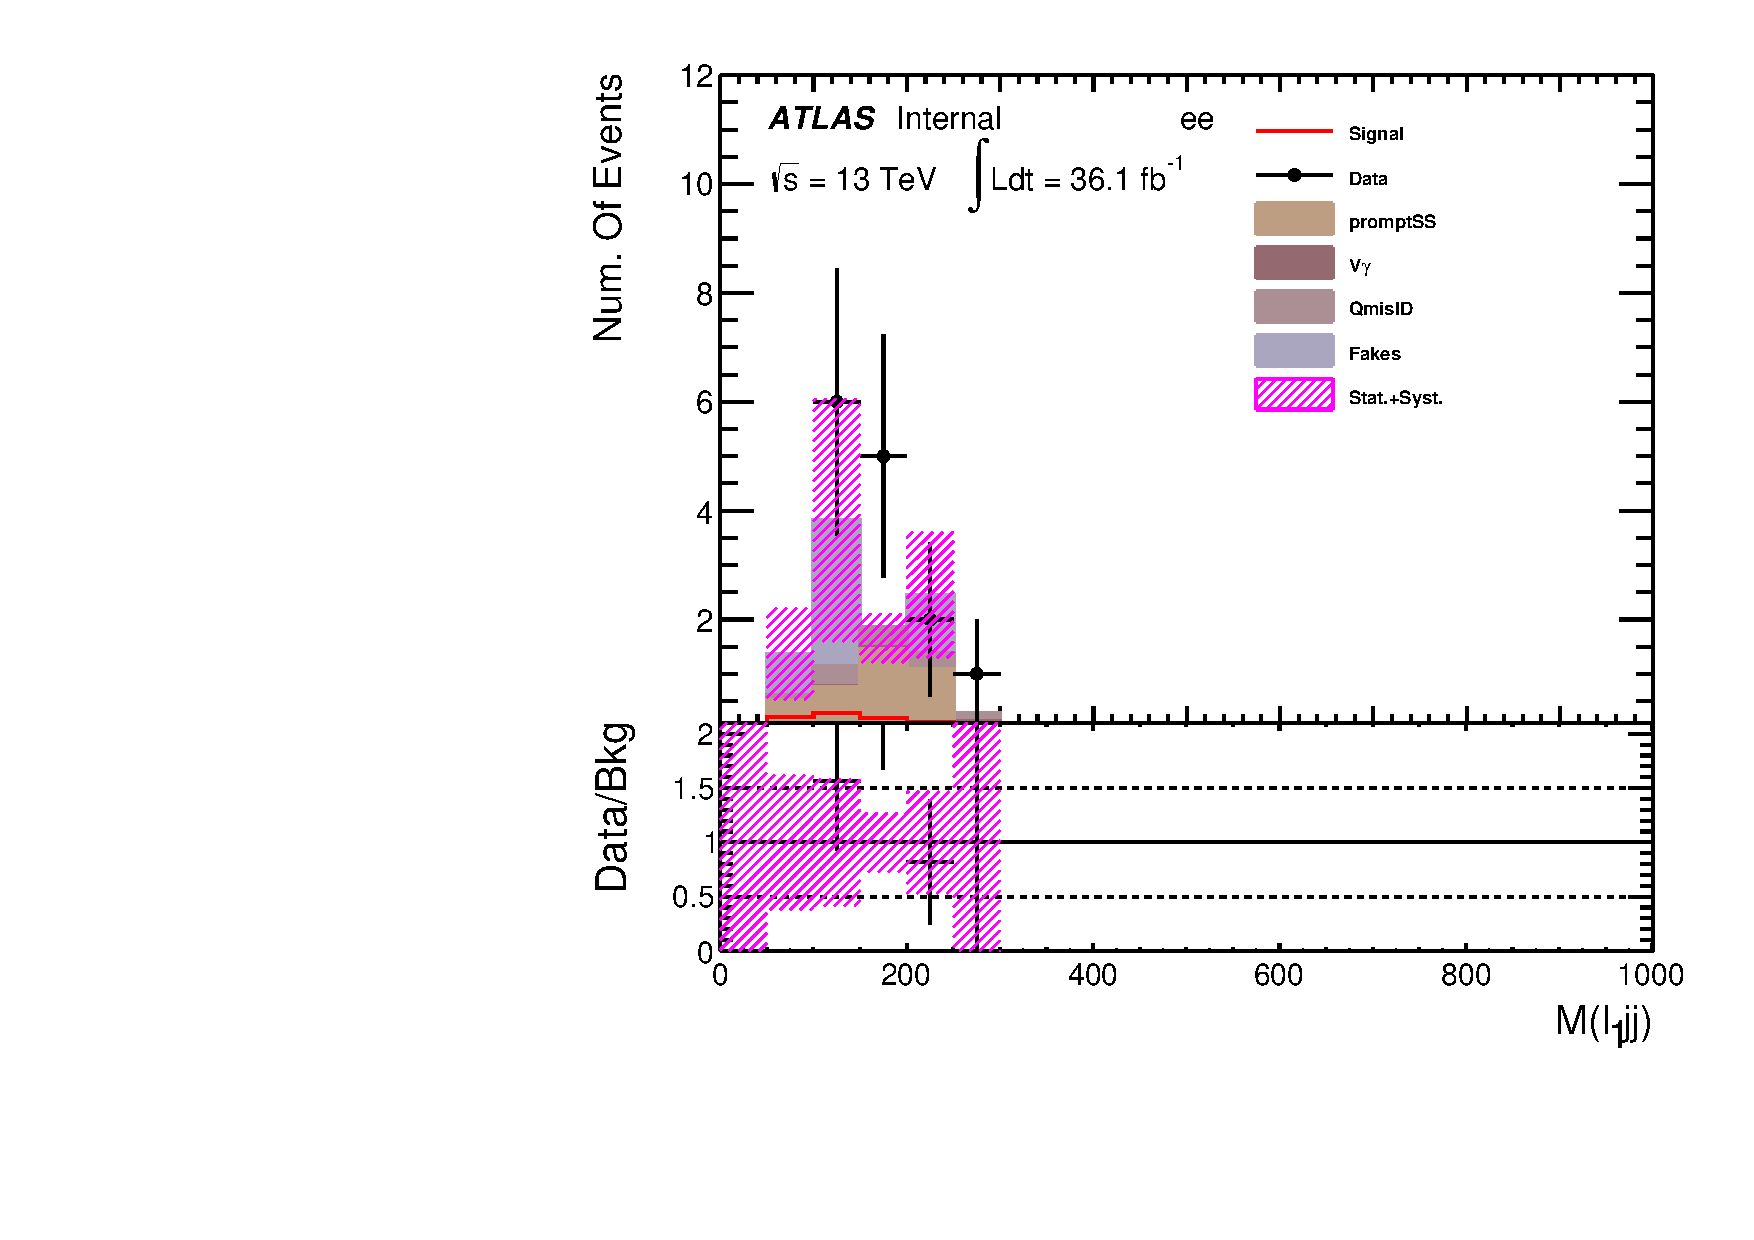
\includegraphics[width=0.9\textwidth,angle=-90]{fig/SigOpt/mH500_m_l1jj_ee.pdf}
 \end{minipage}
 \begin{minipage}[t]{0.33\linewidth}
 \centering
 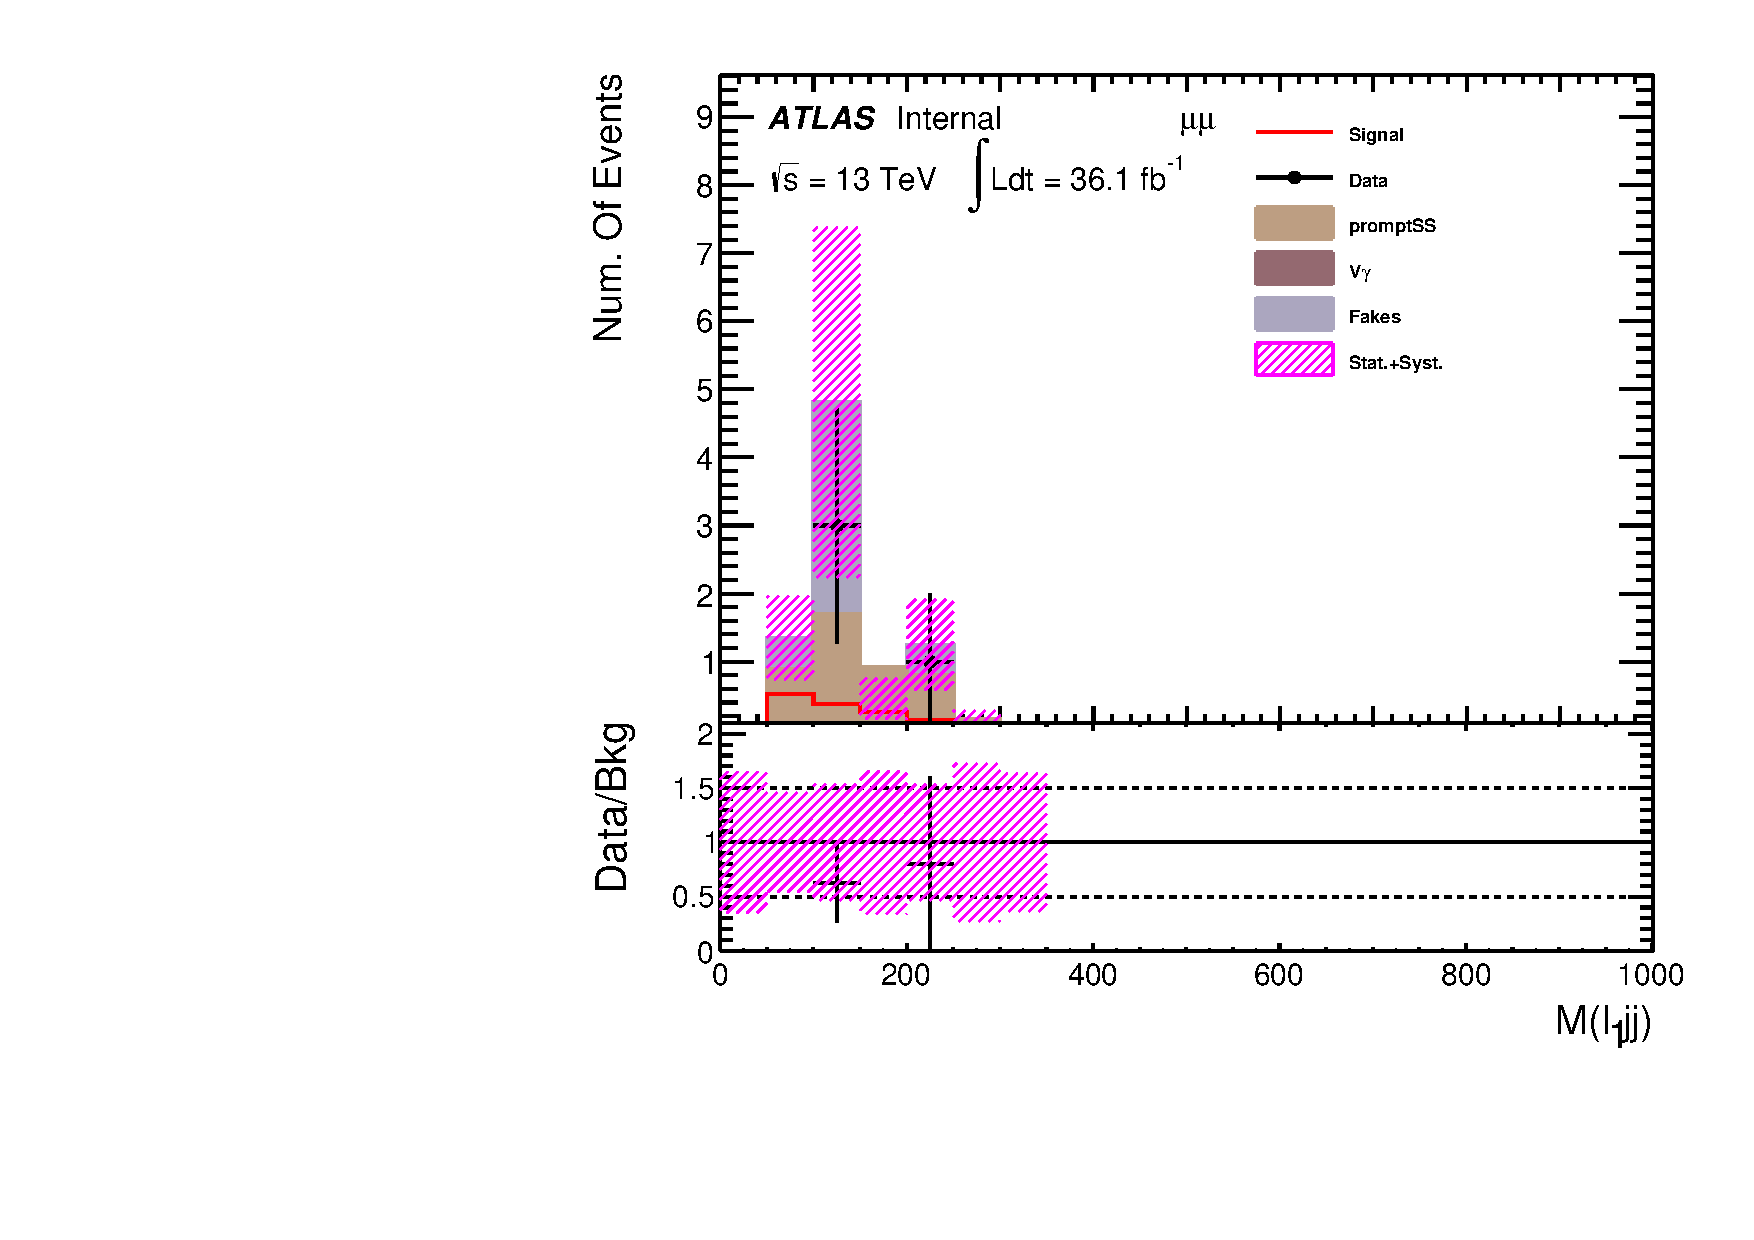
\includegraphics[width=0.9\textwidth,angle=-90]{fig/SigOpt/mH500_m_l1jj_mumu.pdf}
 \end{minipage}
 \begin{minipage}[t]{0.33\linewidth}
 \centering
 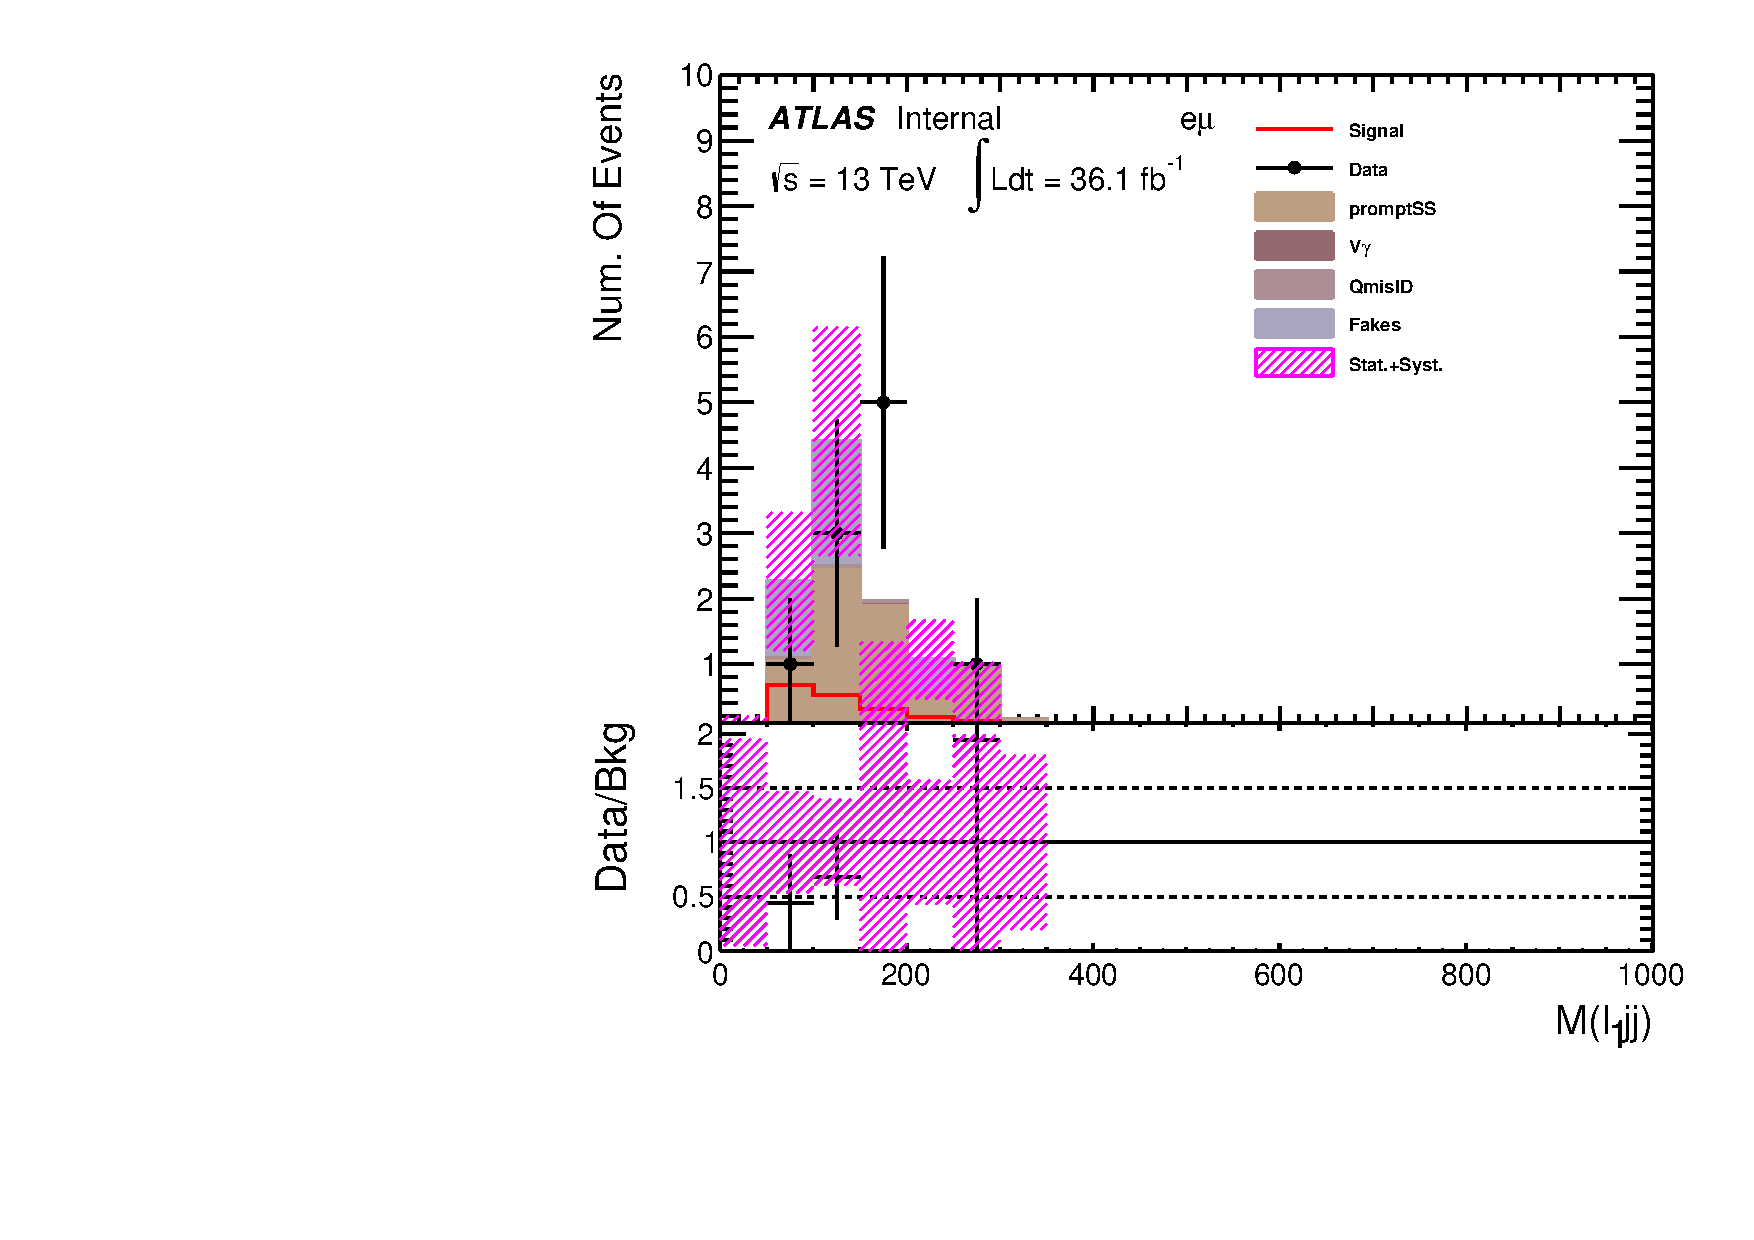
\includegraphics[width=0.9\textwidth,angle=-90]{fig/SigOpt/mH500_m_l1jj_emu.pdf}
 \end{minipage}
 \caption{$m_X$=500 GeV质量点经过优化筛选之后$M(\ell_{1}jj)$分布。}
%\caption{The unblinded $M(\ell_{1}jj)$ distribution after all optimization selections, corresponding to resonance ($m_X$=500 GeV) search.}
\label{fig:SigOpt:mH500_m_l1jj.pdf}
\end{figure}

\clearpage
\subsubsection{$SS$搜寻筛选结果}
\begin{table}[h]
\begin{center}
\tiny\scalebox{0.65}{
\begin{tabular}{c|cccccccc}
\hline
\hline
                           &promptSS  &$V+\gamma$  &QmisID  &Fakes  &Total bkg      \\  
\hline
$\Delta R_{min}(l_{2},j)$ &177.91$\pm$6.06(stat.)$\pm$53.37(syst.)  &84.84$\pm$11.72(stat.)$\pm$42.42(syst.)  &81.84$\pm$0.54(stat.)$\pm$27.01(syst.)  &257.46$\pm$11.79(stat.)$\pm$162.43(syst.)  &602.05$\pm$17.70(stat.)$\mp$73.33(syst1.)$\pm$162.43(syst2.)  \\
\hline
$\Delta R_{min}(l_{1},j)$ &84.62$\pm$3.98(stat.)$\pm$25.39(syst.)  &29.21$\pm$5.40(stat.)$\pm$14.60(syst.)  &29.29$\pm$0.30(stat.)$\pm$9.67(syst.)  &102.28$\pm$7.43(stat.)$\pm$64.53(syst.)  &245.41$\pm$10.02(stat.)$\mp$30.84(syst1.)$\pm$64.53(syst2.) \\
\hline
$M(\ell\ell)$ &29.09$\pm$2.45(stat.)$\pm$8.73(syst.)  &18.51$\pm$4.62(stat.)$\pm$9.25(syst.)  &12.04$\pm$0.15(stat.)$\pm$3.97(syst.)  &58.21$\pm$5.61(stat.)$\pm$36.73(syst.)  &117.84$\pm$7.67(stat.)$\mp$13.32(syst1.)$\pm$36.73(syst2.) \\
\hline
$M(l_{1}jj)$ &10.16$\pm$1.50(stat.)$\pm$3.05(syst.)  &3.34$\pm$1.26(stat.)$\pm$1.67(syst.)  &3.77$\pm$0.06(stat.)$\pm$1.24(syst.)  &20.43$\pm$3.32(stat.)$\pm$12.89(syst.)  &37.69$\pm$3.86(stat.)$\mp$3.69(syst1.)$\pm$12.89(syst2.)  \\
\hline
                          &$X280, S135$  &$X300, S135$  &$X320, S135$ &Observed \\
\hline
$\Delta R_{min}(l_{2},j)$  &3.04$\pm$0.21 &3.54$\pm$0.19   &4.09$\pm$0.22 &647\\
$\Delta R_{min}(l_{1},j)$  &2.48$\pm$0.19 &2.92$\pm$0.18   &3.40$\pm$0.20 &284\\
$M(\ell\ell)$              &2.38$\pm$0.18 &2.61$\pm$0.17   &2.70$\pm$0.18 &128\\
$M(l_{1}jj)$               &1.86$\pm$0.16 &2.10$\pm$0.15   &2.04$\pm$0.16 &50\\
\hline
\hline
\end{tabular}}
\end{center}

\caption{$m_X$=280 GeV, $m_X$=300 GeV and $m_X$=320 GeV(fixing $m_S$=135 GeV) $ee$类别的优化结果。}
%\caption{The unblinded results of the searches for $m_X$=280 GeV, $m_X$=300 GeV and $m_X$=320 GeV(fixing $m_S$=135 GeV) in $ee$ channel.}
\label{cutflow_ee_HSS_lowmass}
\end{table}

\begin{table}[h]
\begin{center}
\tiny\scalebox{0.8}{
\begin{tabular}{c|ccccc}
\hline
\hline
                           &promptSS  &$V+\gamma$  &QmisID  &Fakes  &Total bkg    \\  
\hline
$\Delta R_{min}(l_{2},j)$ &229.53$\pm$6.81(stat.)$\pm$68.86(syst.)  &0.01$\pm$0.01(stat.)$\pm$0.00(syst.)  &0.00$\pm$0.00(stat.)$\pm$0.00(syst.)  &188.45$\pm$9.74(stat.)$\pm$121.65(syst.)  &417.99$\pm$11.88(stat.)$\mp$68.86(syst1.)$\pm$121.65(syst2.) \\
\hline
$\Delta R_{min}(l_{1},j)$ &137.67$\pm$5.13(stat.)$\pm$41.30(syst.)  &0.01$\pm$0.01(stat.)$\pm$0.00(syst.)  &0.00$\pm$0.00(stat.)$\pm$0.00(syst.)  &121.81$\pm$7.83(stat.)$\pm$78.63(syst.)  &259.49$\pm$9.36(stat.)$\mp$41.30(syst1.)$\pm$78.63(syst2.)  \\
\hline
$M(\ell\ell)$ &65.75$\pm$3.73(stat.)$\pm$19.73(syst.)  &0.00$\pm$0.00(stat.)$\pm$0.00(syst.)  &0.00$\pm$0.00(stat.)$\pm$0.00(syst.)  &87.44$\pm$6.63(stat.)$\pm$56.44(syst.)  &153.19$\pm$7.61(stat.)$\mp$19.73(syst1.)$\pm$56.44(syst2.) \\
\hline
$M(l_{1}jj)$ &21.62$\pm$2.05(stat.)$\pm$6.49(syst.)  &0.00$\pm$0.00(stat.)$\pm$0.00(syst.)  &0.00$\pm$0.00(stat.)$\pm$0.00(syst.)  &43.90$\pm$4.70(stat.)$\pm$28.34(syst.)  &65.52$\pm$5.13(stat.)$\mp$6.49(syst1.)$\pm$28.34(syst2.)  \\
\hline
                          &$X280, S135$  &$X300, S135$  &$X320, S135$ &Observed \\
\hline
$\Delta R_{min}(l_{2},j)$  &6.37$\pm$0.27 &7.13$\pm$0.29  &7.74$\pm$0.31 &355\\
$\Delta R_{min}(l_{1},j)$  &5.71$\pm$0.26 &6.23$\pm$0.28  &6.82$\pm$0.29 &210\\
$M(\ell\ell)$              &5.51$\pm$0.26 &5.51$\pm$0.26  &5.43$\pm$0.26 &104\\
$M(l_{1}jj)$               &4.43$\pm$0.24 &4.31$\pm$0.22  &3.96$\pm$0.23 &46\\
\hline
\hline
\end{tabular}}
\end{center}

\caption{$m_X$=280 GeV, $m_X$=300 GeV and $m_X$=320 GeV(fixing $m_S$=135 GeV) $\mu\mu$类别的优化结果。}
%\caption{The unblinded results of the searches for $m_X$=280 GeV, $m_X$=300 GeV and $m_X$=320 GeV(fixing $m_S$=135 GeV) in $\mu\mu$ channel.}
\label{cutflow_mumu_HSS_lowmass}
\end{table}

\begin{table}[h]
\begin{center}
\tiny\scalebox{0.65}{
\begin{tabular}{c|ccccc}
\hline
\hline
                           &promptSS  &$V+\gamma$  &QmisID  &Fakes  &Total bkg   \\  
\hline
$\Delta R_{min}(l_{2},j)$ &305.75$\pm$7.53(stat.)$\pm$91.72(syst.)  &47.54$\pm$6.37(stat.)$\pm$23.77(syst.)  &10.98$\pm$0.19(stat.)$\pm$3.62(syst.)  &174.03$\pm$9.56(stat.)$\pm$79.98(syst.)  &538.30$\pm$13.74(stat.)$\mp$94.82(syst1.)$\pm$79.98(syst2.)  \\
\hline
$\Delta R_{min}(l_{1},j)$ &155.59$\pm$5.15(stat.)$\pm$46.68(syst.)  &19.51$\pm$4.02(stat.)$\pm$9.76(syst.)  &5.65$\pm$0.13(stat.)$\pm$1.87(syst.)  &92.23$\pm$6.96(stat.)$\pm$42.10(syst.)  &272.99$\pm$9.54(stat.)$\mp$47.72(syst1.)$\pm$42.10(syst2.)  \\
\hline
$M(\ell\ell)$ &69.36$\pm$3.51(stat.)$\pm$20.81(syst.)  &12.81$\pm$3.74(stat.)$\pm$6.41(syst.)  &1.40$\pm$0.04(stat.)$\pm$0.46(syst.)  &66.56$\pm$5.91(stat.)$\pm$30.43(syst.)  &150.14$\pm$7.83(stat.)$\mp$21.78(syst1.)$\pm$30.43(syst2.)   \\
\hline
$M(l_{1}jj)$ &25.91$\pm$2.24(stat.)$\pm$7.77(syst.)  &4.70$\pm$1.66(stat.)$\pm$2.35(syst.)  &0.49$\pm$0.02(stat.)$\pm$0.16(syst.)  &39.17$\pm$4.54(stat.)$\pm$18.25(syst.)  &70.27$\pm$5.33(stat.)$\mp$8.12(syst1.)$\pm$18.25(syst2.)  \\
\hline
                          &$X280, S135$  &$X300, S135$  &$X320, S135$ &Observed \\
\hline
$\Delta R_{min}(l_{2},j)$  &8.34$\pm$0.33   &9.25$\pm$0.33   &10.86$\pm$0.40 &649\\
$\Delta R_{min}(l_{1},j)$  &6.87$\pm$0.29   &7.74$\pm$0.31   &8.98$\pm$0.37  &302\\
$M(\ell\ell)$              &6.52$\pm$0.28   &6.87$\pm$0.29   &7.18$\pm$0.32  &155\\
$M(l_{1}jj)$               &5.15$\pm$0.23   &5.46$\pm$0.26   &5.37$\pm$0.28  &62\\
\hline
\hline
\end{tabular}}
\end{center}

\caption{$m_X$=280 GeV, $m_X$=300 GeV and $m_X$=320 GeV(fixing $m_S$=135 GeV) $e\mu$类别的优化结果。}
%\caption{The unblinded results of the searches for $m_X$=280 GeV, $m_X$=300 GeV and $m_X$=320 GeV(fixing $m_S$=135 GeV) in $e\mu$ channel.}
\label{cutflow_emu_HSS_lowmass}
\end{table}

\begin{figure}[h]
\begin{minipage}[t]{0.33\linewidth}
 \centering
 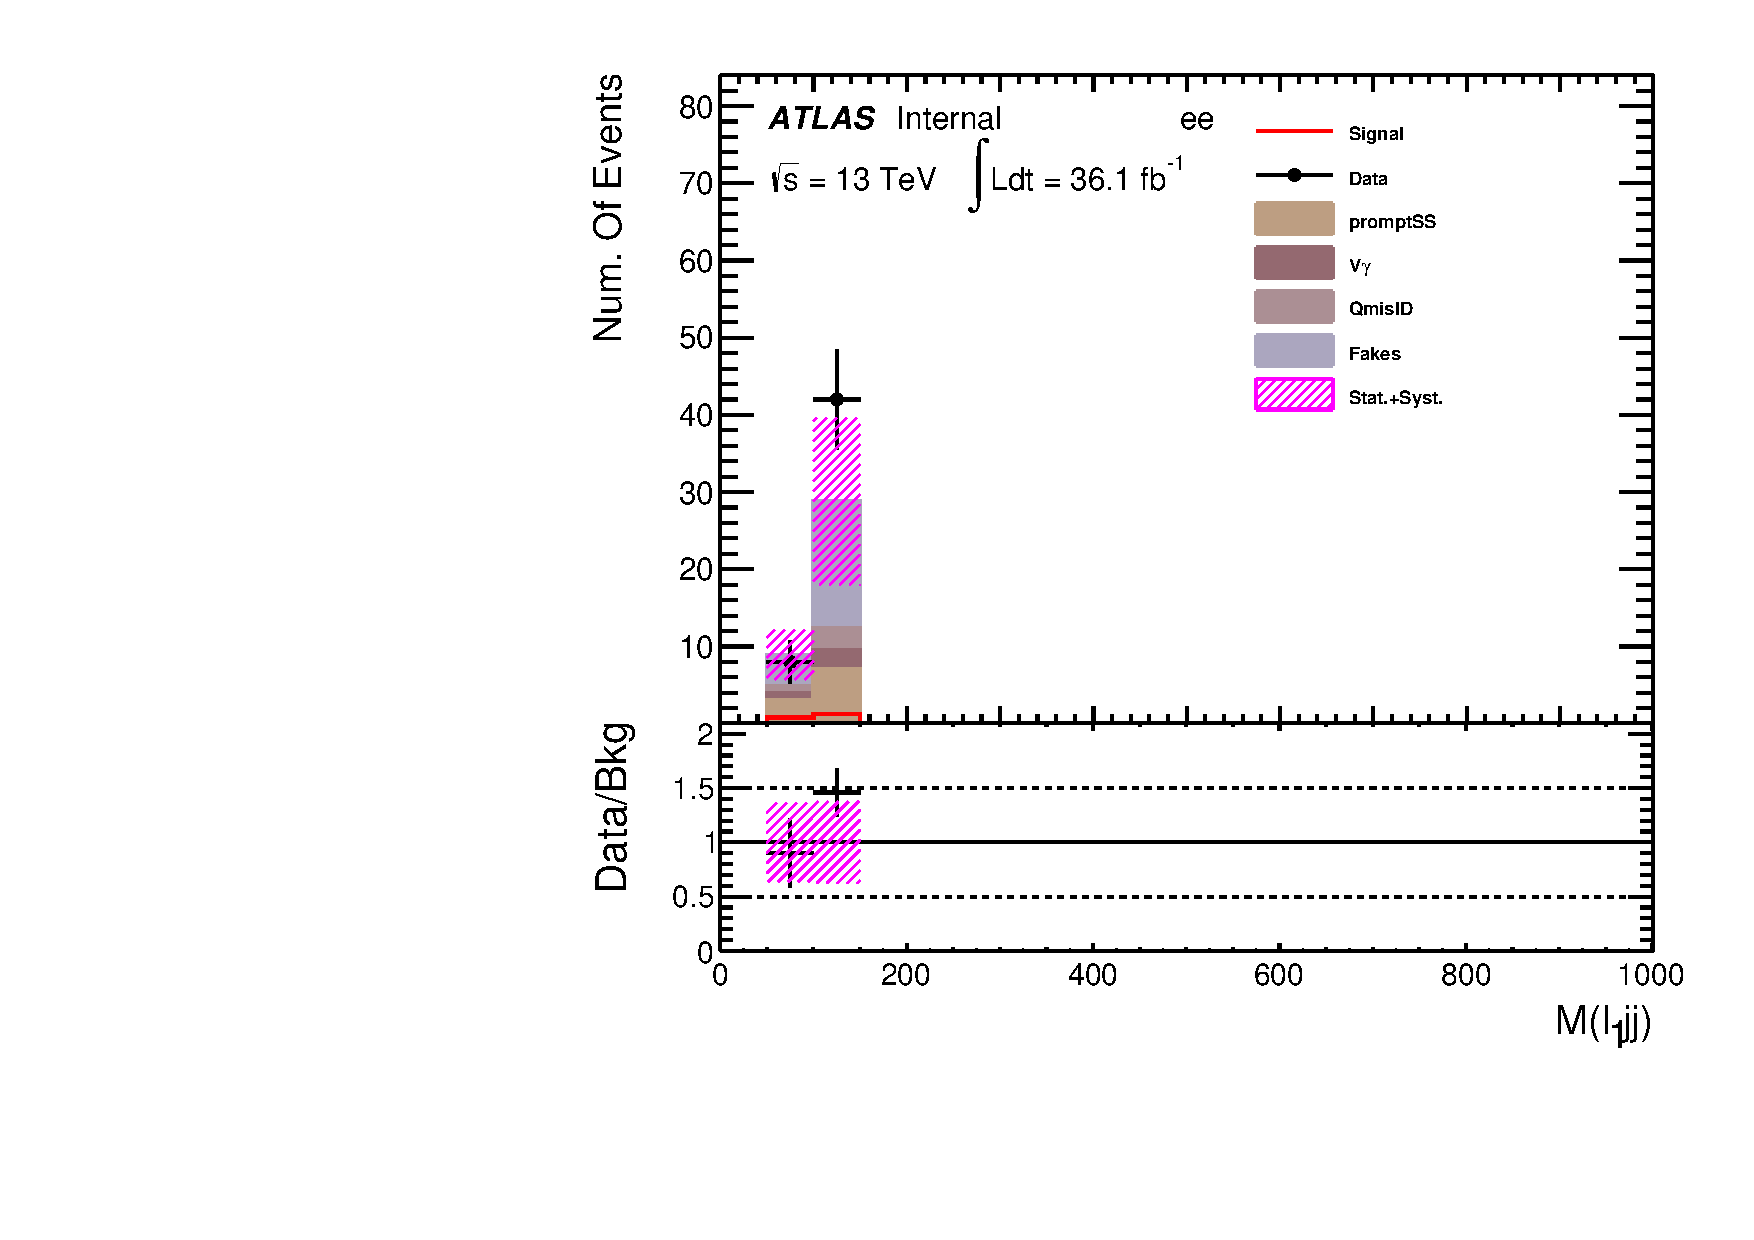
\includegraphics[width=0.9\textwidth,angle=-90]{fig/SigOpt/H300_S135_m_l1jj_ee.pdf}
 \end{minipage}
 \begin{minipage}[t]{0.33\linewidth}
 \centering
 \includegraphics[width=0.9\textwidth,angle=-90]{fig/SigOpt/H300_S135_m_l1jj_mumu.pdf}
 \end{minipage}
 \begin{minipage}[t]{0.33\linewidth}
 \centering
 \includegraphics[width=0.9\textwidth,angle=-90]{fig/SigOpt/H300_S135_m_l1jj_emu.pdf}
 \end{minipage}
 \caption{经过$SS$低质量点优化筛选条件的$M(\ell_{1}jj)$分布,图中展示的信号是$m_X$=300 GeV, $m_S$=135 GeV。}
%\caption{The unblinded $M(\ell_{1}jj)$ distribution after all optimization selections, corresponding to $SS$ low mass search. The signal shown here is $m_X$=300 GeV, $m_S$=135 GeV.}
\label{fig:SigOpt:H300_S135_m_l1jj.pdf}
\end{figure}

\begin{table}[h]
\begin{center}
\tiny\scalebox{0.65}{
\begin{tabular}{c|ccccc}
\hline
\hline
                           &promptSS  &$V+\gamma$  &QmisID  &Fakes  &Total bkg   \\ 
\hline
$\Delta R_{min}(l_{2},j)$ &67.65$\pm$3.53(stat.)$\pm$20.30(syst.)  &20.22$\pm$4.14(stat.)$\pm$10.11(syst.)  &23.49$\pm$0.31(stat.)$\pm$7.75(syst.)  &84.19$\pm$6.79(stat.)$\pm$58.24(syst.)  &195.54$\pm$8.70(stat.)$\mp$23.96(syst1.)$\pm$58.24(syst2.) \\
\hline
$\Delta R_{min}(l_{1},j)$ &39.86$\pm$2.57(stat.)$\pm$11.96(syst.)  &10.52$\pm$2.58(stat.)$\pm$5.26(syst.)  &13.01$\pm$0.21(stat.)$\pm$4.29(syst.)  &43.87$\pm$4.90(stat.)$\pm$30.35(syst.)  &107.26$\pm$6.11(stat.)$\mp$13.75(syst1.)$\pm$30.35(syst2.)  \\
\hline
$M(\ell\ell)$ &22.40$\pm$2.12(stat.)$\pm$6.72(syst.)  &7.57$\pm$2.41(stat.)$\pm$3.79(syst.)  &8.57$\pm$0.15(stat.)$\pm$2.83(syst.)  &35.70$\pm$4.42(stat.)$\pm$24.70(syst.)  &74.24$\pm$5.47(stat.)$\mp$8.21(syst1.)$\pm$24.70(syst2.)    \\
\hline
$M(l_{1}jj)$ &11.57$\pm$1.34(stat.)$\pm$3.47(syst.)  &3.51$\pm$1.21(stat.)$\pm$1.75(syst.)  &4.22$\pm$0.08(stat.)$\pm$1.39(syst.)  &24.59$\pm$3.67(stat.)$\pm$17.01(syst.)  &43.89$\pm$4.09(stat.)$\mp$4.13(syst1.)$\pm$17.01(syst2.)  \\
\hline
                             &X340, S135  &X340, S145  &X340, S155  &X340, S165 &Observed\\
\hline
$\Delta R_{min}(l_{2},j)$  &2.95$\pm$0.20 &9.19$\pm$0.52 &17.48$\pm$0.94 &29.64$\pm$1.58 \\
$\Delta R_{min}(l_{1},j)$  &2.56$\pm$0.19 &8.26$\pm$0.50 &15.41$\pm$0.86 &27.84$\pm$1.51 \\
$M(\ell\ell)$              &2.38$\pm$0.19 &7.83$\pm$0.49 &15.31$\pm$0.85 &27.84$\pm$1.51 \\
$M(l_{1}jj)$               &2.22$\pm$0.18 &7.15$\pm$0.47 &13.95$\pm$0.82 &25.66$\pm$1.44 \\
\hline
\hline
\end{tabular}}
\end{center}

\caption{$m_S$=135 GeV, $m_S$=145 GeV, $m_S$=155 GeV and $m_S$=165 GeV(fixing $m_X$=340 GeV) $ee$类别的优化结果。}
%\caption{The unblinded results of the searches for $m_S$=135 GeV, $m_S$=145 GeV, $m_S$=155 GeV and $m_S$=165 GeV(fixing $m_X$=340 GeV) in $ee$ channel.}
\label{cutflow_ee_HSS_highmass}
\end{table}

\begin{table}[h]
\begin{center}
\tiny\scalebox{0.65}{
\begin{tabular}{c|ccccc}
\hline
\hline
                           &promptSS  &$V+\gamma$  &QmisID  &Fakes  &Total bkg    \\  
\hline
$\Delta R_{min}(l_{2},j)$ &116.18$\pm$4.57(stat.)$\pm$34.85(syst.)  &0.01$\pm$0.01(stat.)$\pm$0.00(syst.)  &0.00$\pm$0.00(stat.)$\pm$0.00(syst.)  &102.27$\pm$6.82(stat.)$\pm$73.42(syst.)  &218.45$\pm$8.21(stat.)$\mp$34.85(syst1.)$\pm$73.42(syst2.)  \\
\hline
$\Delta R_{min}(l_{1},j)$ &72.61$\pm$3.46(stat.)$\pm$21.78(syst.)  &0.01$\pm$0.01(stat.)$\pm$0.00(syst.)  &0.00$\pm$0.00(stat.)$\pm$0.00(syst.)  &64.78$\pm$5.43(stat.)$\pm$46.50(syst.)  &137.39$\pm$6.44(stat.)$\mp$21.78(syst1.)$\pm$46.50(syst2.)  \\
\hline
$M(\ell\ell)$ &39.34$\pm$2.56(stat.)$\pm$11.80(syst.)  &0.01$\pm$0.01(stat.)$\pm$0.00(syst.)  &0.00$\pm$0.00(stat.)$\pm$0.00(syst.)  &55.61$\pm$5.03(stat.)$\pm$39.92(syst.)  &94.96$\pm$5.64(stat.)$\mp$11.80(syst1.)$\pm$39.92(syst2.)  \\
\hline
$M(l_{1}jj)$ &22.92$\pm$1.79(stat.)$\pm$6.88(syst.)  &0.00$\pm$0.00(stat.)$\pm$0.00(syst.)  &0.00$\pm$0.00(stat.)$\pm$0.00(syst.)  &39.33$\pm$4.23(stat.)$\pm$28.24(syst.)  &62.25$\pm$4.59(stat.)$\mp$6.88(syst1.)$\pm$28.24(syst2.)  \\
\hline
                             &X340, S135  &X340, S145  &X340, S155  &X340, S165 &Observed\\
\hline
$\Delta R_{min}(l_{2},j)$  &5.92$\pm$0.26 &19.02$\pm$0.83  &38.96$\pm$1.50 &64.54$\pm$2.19 &172\\
$\Delta R_{min}(l_{1},j)$  &5.39$\pm$0.25 &17.52$\pm$0.81  &36.36$\pm$1.47 &61.47$\pm$2.14 &113\\
$M(\ell\ell)$              &4.89$\pm$0.24 &16.51$\pm$0.79  &35.05$\pm$1.44 &61.31$\pm$2.14 &66\\
$M(l_{1}jj)$               &4.34$\pm$0.23 &14.90$\pm$0.75  &32.26$\pm$1.39 &56.55$\pm$2.06 &38\\
\hline
\hline
\end{tabular}}
\end{center}

\caption{$m_S$=135 GeV, $m_S$=145 GeV, $m_S$=155 GeV and $m_S$=165 GeV(fixing $m_X$=340 GeV) $\mu\mu$类别的优化结果。}
%\caption{The unblinded results of the searches for $m_S$=135 GeV, $m_S$=145 GeV, $m_S$=155 GeV and $m_S$=165 GeV(fixing $m_X$=340 GeV) in $\mu\mu$ channel.}
\label{cutflow_mumu_HSS_highmass}
\end{table}

\begin{table}[h]
\begin{center}
\tiny\scalebox{0.65}{
\begin{tabular}{c|ccccc}
\hline
\hline
                           &promptSS  &$V+\gamma$  &QmisID  &Fakes  &Total bkg   \\  
\hline
$\Delta R_{min}(l_{2},j)$ &158.05$\pm$5.26(stat.)$\pm$47.42(syst.)  &24.53$\pm$4.99(stat.)$\pm$12.26(syst.)  &5.42$\pm$0.13(stat.)$\pm$1.79(syst.)  &79.82$\pm$6.36(stat.)$\pm$39.91(syst.)  &267.81$\pm$9.65(stat.)$\mp$49.01(syst1.)$\pm$39.91(syst2.)  \\
\hline
$\Delta R_{min}(l_{1},j)$ &93.10$\pm$4.03(stat.)$\pm$27.93(syst.)  &13.51$\pm$3.65(stat.)$\pm$6.76(syst.)  &3.28$\pm$0.10(stat.)$\pm$1.08(syst.)  &49.78$\pm$5.03(stat.)$\pm$25.05(syst.)  &159.67$\pm$7.41(stat.)$\mp$28.76(syst1.)$\pm$25.05(syst2.)  \\
\hline
$M(\ell\ell)$ &65.27$\pm$3.46(stat.)$\pm$19.58(syst.)  &10.94$\pm$3.53(stat.)$\pm$5.47(syst.)  &1.47$\pm$0.04(stat.)$\pm$0.49(syst.)  &42.40$\pm$4.64(stat.)$\pm$21.29(syst.)  &120.08$\pm$6.78(stat.)$\mp$20.34(syst1.)$\pm$21.29(syst2.)  \\
\hline
$M(l_{1}jj)$ &23.53$\pm$2.01(stat.)$\pm$7.06(syst.)  &3.53$\pm$1.29(stat.)$\pm$1.76(syst.)  &0.52$\pm$0.02(stat.)$\pm$0.17(syst.)  &25.49$\pm$3.64(stat.)$\pm$13.58(syst.)  &53.07$\pm$4.36(stat.)$\mp$7.28(syst1.)$\pm$13.58(syst2.)  \\
\hline
                             &X340, S135  &X340, S145  &X340, S155  &X340, S165 &Observed\\
\hline
$\Delta R_{min}(l_{2},j)$  &8.50$\pm$0.34 &24.75$\pm$0.83 &49.33$\pm$1.64 &85.30$\pm$2.45 &308\\
$\Delta R_{min}(l_{1},j)$  &7.51$\pm$0.31 &21.64$\pm$0.78 &43.74$\pm$1.54 &79.38$\pm$2.37 &179\\
$M(\ell\ell)$              &7.41$\pm$0.31 &21.53$\pm$0.78 &43.57$\pm$1.54 &79.38$\pm$2.37 &131\\
$M(l_{1}jj)$               &5.58$\pm$0.27 &16.64$\pm$0.68 &35.70$\pm$1.41 &69.41$\pm$2.23 &64\\
\hline
\hline
\end{tabular}}
\end{center}

\caption{$m_S$=135 GeV, $m_S$=145 GeV, $m_S$=155 GeV and $m_S$=165 GeV(fixing $m_X$=340 GeV) $e\mu$类别的优化结果。}
%\caption{The unblinded results of the searches for $m_S$=135 GeV, $m_S$=145 GeV, $m_S$=155 GeV and $m_S$=165 GeV(fixing $m_X$=340 GeV) in $e\mu$ channel.}
\label{cutflow_emu_HSS_highmass}
\end{table}

\begin{figure}[h]
\begin{minipage}[t]{0.33\linewidth}
 \centering
 \includegraphics[width=0.9\textwidth,angle=-90]{fig/SigOpt/H340_S145_m_l1jj_ee.pdf}
 \end{minipage}
 \begin{minipage}[t]{0.33\linewidth}
 \centering
 \includegraphics[width=0.9\textwidth,angle=-90]{fig/SigOpt/H340_S145_m_l1jj_mumu.pdf}
 \end{minipage}
 \begin{minipage}[t]{0.33\linewidth}
 \centering
 \includegraphics[width=0.9\textwidth,angle=-90]{fig/SigOpt/H340_S145_m_l1jj_emu.pdf}
 \end{minipage}
  \caption{经过$SS$高质量点优化筛选条件的$M(\ell_{1}jj)$分布,图中展示的信号是$m_X$=340 GeV, $m_S$=145 GeV。}
%\caption{The unblinded $M(\ell_{1}jj)$ distribution after all optimization selections, corresponding to $SS$ high mass search. The signal shown here is $m_X$=340 GeV, $m_S$=145 GeV.}
\label{fig:SigOpt:H340_S165_m_l1jj.pdf}
\end{figure}
